\documentclass{article} % For LaTeX2e
\usepackage[preprint]{colm2026_conference}

\usepackage{microtype}
\usepackage{hyperref}
\usepackage{url}
\usepackage{booktabs}
\usepackage{lineno}
\usepackage{amsmath,amsfonts,amssymb}
\usepackage{tikz}
\usetikzlibrary{trees, shapes.geometric, arrows.meta, positioning, calc, shadows, backgrounds, fit}
\usepackage[edges]{forest}
\usepackage{enumitem}
\usepackage{multirow}
\usepackage{graphicx}
\usepackage{placeins}
\usepackage{fontawesome}

% === Figure fonts and colors (shared by inline TikZ figures) ===
\usepackage{tgheros}
\usepackage{sansmath}
\definecolor{deepblue}{HTML}{1A5276}
\definecolor{midblue}{HTML}{2980B9}
\definecolor{lightblue}{HTML}{AED6F1}
\definecolor{lightblue2}{HTML}{D4E6F1}
\definecolor{deeppurple}{HTML}{6C3483}
\definecolor{deepgray}{HTML}{2C3E50}
\definecolor{midpurple}{HTML}{8E44AD}
\definecolor{lightpurple}{HTML}{D2B4DE}
\definecolor{deeporange}{HTML}{B9470B}
\definecolor{midorange}{HTML}{E67E22}
\definecolor{lightorange}{HTML}{F5CBA7}
\definecolor{coralpink}{HTML}{E74C3C}
\definecolor{midgray}{HTML}{7F8C8D}
\definecolor{panelbg}{HTML}{F5F8FC}
\definecolor{darkblue}{rgb}{0, 0, 0.5}
\hypersetup{colorlinks=true, citecolor=darkblue, linkcolor=darkblue, urlcolor=darkblue}

\title{A Survey of On-Policy Distillation for Large Language Models}

\author{Mingyang Song \& Mao Zheng \\
Large Language Model Department \\Tencent, China\\
\texttt{nickmysong@tencent.com}}

\newcommand{\fix}{\marginpar{FIX}}
\newcommand{\new}{\marginpar{NEW}}

% Math macros
\newcommand{\E}{\mathbb{E}}
\newcommand{\KL}{D_{\mathrm{KL}}}
\newcommand{\ptheta}{p_\theta}
\newcommand{\pteacher}{p_T}
\newcommand{\pdata}{p_{\mathrm{data}}}
\newcommand{\loss}{\mathcal{L}}
\DeclareMathOperator*{\argmin}{arg\,min}
\DeclareMathOperator*{\argmax}{arg\,max}

\begin{document}
\maketitle

\begin{abstract}
As Large Language Models (LLMs) continue to grow in both capability and cost, the transfer of frontier capabilities into smaller, deployable students has become a central engineering problem, and knowledge distillation has become the natural vehicle for this transfer. Yet the form that now dominates industrial pipelines, static imitation of teacher-generated text, carries a structural weakness that becomes increasingly severe as tasks grow longer and more reasoning-intensive. Because the student is trained on flawless teacher prefixes but must generate its own at inference, small mistakes accumulate into trajectories it has never been taught to recover from, and the resulting exposure bias scales with the square of sequence length. On-Policy Distillation (OPD) reorganizes the training loop around this observation by asking the teacher to provide feedback on what the student \emph{actually produces}, shrinking the compounding term to linear and turning distillation from one-shot behavior copying into an interactive correction process. The resulting literature has expanded rapidly along divergence design, reward-guided optimization, and self-play, yet contributions remain scattered across the knowledge distillation, RLHF, and imitation learning communities with no unified treatment. This survey brings them under a common analytical lens. We cast OPD as $f$-divergence minimization over student-sampled trajectories, organize the field along the practitioner's actual decision chain of what to optimize, where the signal comes from, and how to stabilize the loop in practice, and consolidate success conditions, recurring failure modes, and the formal equivalence between OPD and KL-constrained reinforcement learning. We close with the open problems that emerge from this synthesis, from distillation scaling laws and uncertainty-aware feedback to agent-level distillation and the dissolving boundary between knowledge distillation and RL.
\end{abstract}

% === GitHub Banner ===
\vspace{-0.3em}
\begin{center}
\begin{tikzpicture}
  \node[draw=midblue!60, fill=lightblue2!40, rounded corners=6pt, inner sep=8pt, line width=0.8pt] (box) {
    \begin{minipage}{0.82\textwidth}
      \centering
      {\sffamily\small%
        \textcolor{deepblue}{\textbf{\faGithub\;\; Awesome List \& Paper Collection}}\\[3pt]
        \textcolor{midblue}{\url{https://github.com/nick7nlp/Awesome-LLM-On-Policy-Distillation}}
      }
    \end{minipage}
  };
\end{tikzpicture}
\end{center}
\vspace{-0.3em}

\section{Introduction}
\label{sec:intro}

The frontier of Large Language Models (LLMs) has advanced at a pace that few other areas of machine learning have matched, with recent systems achieving state-of-the-art performance across reasoning, code generation, and multilingual benchmarks~\citep{2505.09388,2501.12948,2408.00118}. This progress has come at a cost that only a handful of organizations can sustain. Capability transfer from large frontier models into smaller deployable students has moved from academic curiosity to one of the load-bearing techniques of the modern LLM pipeline. Knowledge distillation, first formalized by \citet{hinton2015distilling} as a way for a student to inherit the soft output structure of a teacher, has shifted in character with it. What began as a model compression technique for transferring knowledge within the same architecture has become a general mechanism for moving capabilities across model scales and architectural families. The release of DeepSeek-R1~\citep{2501.12948} made this shift concrete, distilling a 671B mixture-of-experts teacher into dense students spanning 1.5B to 70B parameters while preserving long chain-of-thought reasoning largely intact.

The dominant recipe behind such successes is, however, deceptively fragile. In almost all large-scale pipelines, distillation proceeds \emph{off-policy}. The student is trained to match the teacher's next-token distribution over a fixed corpus, typically the original pre-training data or traces generated in advance by the teacher, and every gradient step conditions on flawless teacher prefixes. At inference, this assumption breaks. The student must generate autoregressively from its own partial outputs, and any divergence between the training states and the states it visits at deployment time translates into compounding error along the trajectory. This is a textbook instance of the \emph{compounding error} identified in interactive imitation learning~\citep{ross2011reduction}, where autoregressive generation amplifies the distribution mismatch quadratically in sequence length, producing an expected discrepancy of $O(\epsilon T^2)$ over a horizon $T$. The consequences are most visible on reasoning tasks, where a single early misstep can derail an entire proof or program. \citet{2305.15717} warned that off-policy imitation of proprietary LLMs often yields students that reproduce surface style without acquiring the underlying reasoning competence.

Resolving this mismatch requires changing \emph{where} the training data comes from rather than \emph{what} is being matched. \textbf{On-Policy Distillation (OPD)} does exactly that by shifting the sampling distribution from a static corpus to the student's own evolving policy. The student proposes trajectories, populates the very states it would visit at deployment, and receives teacher feedback on those states rather than on idealized expert prefixes. Depending on the available access, this feedback ranges from full token-level distributions in white-box settings~\citep{2306.13649,2306.08543}, through scalar rewards or pairwise preferences when only black-box APIs are available~\citep{2511.10643,2305.12870}, to contrastive signals the model derives from its own outputs in teacher-free settings~\citep{2401.01335}. The theoretical payoff mirrors the classical DAgger result~\citep{ross2011reduction}, where querying an expert on the learner's own visited states reduces the $O(\epsilon T^2)$ compounding of off-policy imitation to $O(\epsilon T)$. Translated into autoregressive language modeling, this turns distillation from a single-pass matching problem into an iterative optimization loop in which the training distribution co-evolves with the model, exposing and correcting distributional gaps that static training would never surface.

This reformulation has produced a body of work best understood as a series of design choices progressively surfaced. Early methods focused on \emph{how} to sample and \emph{which} divergence to apply on student trajectories~\citep{2306.13649,2306.08543,2402.03898}, establishing that the optimal divergence depends on where in the sequence one is training and what kind of supervision the teacher can provide. A parallel line of work established that the resulting objective is formally equivalent to a KL-constrained form of reinforcement learning~\citep{2602.12125}, dissolving what had looked like a boundary between two separate research communities. A third branch showed that the ``teacher'' need not be external at all, with methods such as SPIN~\citep{2401.01335} and OPSD~\citep{2601.18734} demonstrating that a model can bootstrap improvement from its own generations by exploiting asymmetries in its output distribution across contexts. These ideas have since moved from papers into production pipelines, with Qwen3~\citep{2505.09388}, DeepSeek-V4~\citep{deepseekv4}, Gemma~2~\citep{2408.00118}, and MiMo-V2~\citep{2601.02780} all treating OPD as a core training ingredient. The convergence is not coincidental. These systems span mixture-of-experts and dense architectures, proprietary and open-weight release strategies, yet all face the same structural problem once reasoning chains grow long enough for compounding error to dominate. DeepSeek-V4 went furthest, replacing its mixed RL stage with pure multi-teacher OPD for model consolidation.

GKD~\citep{2306.13649}, alongside the concurrent MiniLLM~\citep{2306.08543}, introduced the first on-policy frameworks for autoregressive LM distillation in mid-2023, and fewer than two years later the literature has expanded to over one hundred papers spanning divergence design, reward-guided optimization, self-play, multi-teacher debate, agentic trajectory distillation, and cross-modal transfer. The field's center of gravity has shifted accordingly. Where early work asked whether on-policy training helps at all, the current frontier asks how to make it efficient enough for trillion-parameter teacher inference, how to extend it beyond single-turn generation into multi-step agent trajectories, and how to unify it with the reinforcement learning pipelines that increasingly share its computational infrastructure. This acceleration tracks a structural trend in LLM development. As models grow more capable and reasoning chains grow longer, the gap between off-policy training states and deployment-time states widens, making on-policy correction architecturally necessary for the next generation of reasoning-capable systems~\citep{2603.25562,deepseekv4}.

Yet the practical success of OPD has outpaced the community's ability to understand it as a single object. Methods approach the same problem through the lenses of knowledge distillation, RLHF, and interactive imitation learning, inheriting different notations, benchmarks, and failure taxonomies from their parent communities. Existing surveys of LLM distillation~\citep{2402.13116} generally retain the classical compression framing, treating off-policy and on-policy methods as interchangeable variants rather than as regimes with materially different theoretical guarantees and failure modes. As a result, no current treatment offers a unified mathematical account of the on-policy dynamics that connect these threads, and no systematic comparison exists across the white-box, black-box, and teacher-free instantiations that a practitioner is likely to weigh against one another in practice.

This survey fills that gap. Our goals are both conceptual and practical, and they are reflected in four contributions that also structure the rest of the paper.
\begin{itemize}[leftmargin=1.5em]
    \item \textbf{A unified theoretical framework.} We recast the transition from off-policy to on-policy distillation as a sequential decision-making problem and show that the core OPD algorithms are instances of $f$-divergence minimization over student-sampled trajectories (Section~\ref{sec:background}). This framework provides a common analytical vocabulary for methods previously studied in isolation and makes their relationships explicit in terms of divergence choice, argument ordering, and sampling mixture.
    \item \textbf{A decision-centric taxonomy.} Rather than grouping methods by surface similarity, we organize them by their role in a practitioner's decision chain (Section~\ref{sec:landscape}), namely objective function design (Section~\ref{sec:objectives}), signal source architecture (Section~\ref{sec:signal}), and training dynamics optimization (Section~\ref{sec:dynamics}). The resulting one-method-one-category classification is aimed directly at the question of \emph{which method to use} given a set of deployment constraints.
    \item \textbf{A theoretical account of failure.} We consolidate the empirical record into a coherent view of when and why OPD breaks down (Section~\ref{sec:understanding}), covering the flawed prefix trap, self-play saturation, diversity collapse, and the calibration-capability gap, and we state formal conditions under which OPD provably improves over off-policy alternatives.
    \item \textbf{Comprehensive coverage and actionable guidance.} We survey the white-box, black-box, and self-distillation regimes within this common framework, summarize them in three comparison tables (Tables~\ref{tab:method_comparison},~\ref{tab:white_box_comparison}, and~\ref{tab:experimental_configs}), and translate the synthesis into a concrete decision tree (Section~\ref{subsec:decision_tree}) that maps deployment constraints to recommended methods and compute budgets.
\end{itemize}

The structure of the paper mirrors this decision-centric logic. Section~\ref{sec:background} develops the mathematical preliminaries, formalizes autoregressive generation as a sequential decision problem, and derives the exposure bias that motivates on-policy training. Section~\ref{sec:landscape} lays out the practitioner-centric landscape and decision tree. Sections~\ref{sec:objectives}--\ref{sec:dynamics} then traverse the decision chain from ``what to optimize'' through ``where the signal comes from'' to ``how to make training work in practice,'' with each section building directly on the choices exposed in the previous one. Section~\ref{sec:understanding} consolidates the theoretical perspectives, showing that the patterns observed across Sections~\ref{sec:objectives}--\ref{sec:dynamics} follow from a small number of unifying principles. Section~\ref{sec:applications} discusses industrial deployments, system-level optimization, and emerging domains, and Section~\ref{sec:future} lays out the open problems that emerge from the synthesis.

Our scope is deliberately centered on the on-policy regime. We cover methods in which the student generates its own training data during distillation, and we include work from adjacent fields such as imitation learning, online RL, and preference optimization whenever it operates on student-generated data under teacher or verifier supervision. We correspondingly set aside generic off-policy KD, compression techniques that are orthogonal to the training paradigm such as pruning and quantization, and inference-time methods that leave model weights unchanged.

\section{Background and Unified Math}
\label{sec:background}

To understand why on-policy training is necessary, we formalize the compounding geometry of autoregressive generation. We begin with classical KD and its limitations, then establish the unified $f$-divergence framework that subsumes modern OPD objectives.

\textbf{Defining ``on-policy.''}  A distillation method is \emph{on-policy} if the training data for the student is sampled from the student's own current policy $\ptheta$ at training time, rather than from a fixed external corpus $\mathcal{D}$ or from the teacher's generation distribution $\pteacher$. Formally, on-policy training optimizes:
\begin{equation}
    \min_\theta \E_{x \sim \mathcal{D}}\, \E_{y \sim \ptheta(\cdot|x)} \left[ \mathcal{L}(y, x; \theta, T) \right]
\end{equation}
where $\mathcal{L}$ is the distillation loss (divergence, reward, or hybrid). The key distinction is that the \emph{outer} expectation is over the student's own generations, not a static dataset. This creates a non-stationary optimization landscape because as $\theta$ updates, the data distribution $\ptheta$ shifts, requiring fresh rollouts at each training step. The computational cost of this fresh generation is the central systems-level challenge of OPD (Section~\ref{subsec:compute}).

\textbf{Notation.} Throughout this survey, we use lowercase $p$ for token-level conditional distributions ($\pteacher(\cdot|x, y_{<t})$ for teacher, $\ptheta(\cdot|x, y_{<t})$ for student) and uppercase $P$ for sequence-level distributions ($P_T(y|x)$, $P_\theta(y|x)$). $\mathcal{D}$ denotes the training dataset, $\pdata$ the data distribution, and $|V|$ the vocabulary size. $\KL$ and $D_f$ denote KL divergence and general $f$-divergence respectively. In the RL formalization, $\pi$ denotes policies and $R(x,y)$ the outcome reward. When discussing individual methods, we follow each paper's conventions where clarity demands.

\subsection{Classical Knowledge Distillation}

The original KD formulation~\citep{hinton2015distilling} trains the student to match the teacher's temperature-softened output distribution:
\begin{equation}
    p_T^{(\tau)}(y|x) = \frac{\exp(z_y / \tau)}{\sum_{j} \exp(z_j / \tau)}
\end{equation}
where $z_y$ are the teacher's logits and $\tau > 1$ is a temperature parameter. When $\tau \to \infty$, the softened distribution approaches a uniform distribution over the vocabulary, exposing the teacher's ``dark knowledge'' about inter-class similarities that hard labels hide. The gradient of the distillation loss with respect to the student's logits $z_i^{\mathcal{S}}$ shows why temperature matters:
\begin{equation}
    \frac{\partial \loss_{\text{KD}}}{\partial z_i^{\mathcal{S}}} = \frac{1}{\tau}(p_i^{\mathcal{S}} - p_i^{\mathcal{T}})
\end{equation}
In the high-temperature limit ($\tau \to \infty$), a Taylor expansion $\exp(z_i/\tau) \approx 1 + z_i/\tau$ together with the zero-mean assumption $\sum_i z_i^{\mathcal{S}} = \sum_i z_i^{\mathcal{T}} = 0$ reduces the gradient to $\frac{1}{|V|\tau^2}(z_i^{\mathcal{S}} - z_i^{\mathcal{T}})$~\citep{hinton2015distilling}, so classical KD in this regime is equivalent to minimizing the mean squared error between raw logits. This forces the student to replicate the teacher's \emph{entire} logit structure, transferring both primary predictive modes and nuanced sub-optimal probability masses (the ``dark knowledge''). The $1/\tau^2$ factor explains why the soft-target term is commonly upweighted by $\tau^2$ relative to the hard-label cross-entropy in the combined KD objective. In practice, LLM distillation operates at $\tau = 1$ or low-to-moderate temperatures~\citep{2402.11890} because the large vocabulary ($|V| > 30{,}000$) already produces richly structured non-peak probabilities without explicit softening, and higher temperatures may amplify noise in the teacher's poorly calibrated tail distribution.

For autoregressive LLMs, the token-level distillation loss factors as:
\begin{equation}
    \loss_{\text{Token-KD}} = \E_{x, y \sim \mathcal{D}} \left[ \sum_{t=1}^{|y|} \KL(\pteacher(\cdot | x, y_{<t}) \parallel \ptheta(\cdot | x, y_{<t})) \right]
\end{equation}
This is computationally tractable because it relies on static, pre-computed prefixes from the dataset, but it optimizes next-token accuracy while assuming an error-free history $y_{<t}$. \citet{kim2016sequence} extended this to Sequence-Level Knowledge Distillation (Seq-KD), which instead minimizes the global KL divergence over the entire sequence space:
\begin{equation}
    \loss_{\text{Seq-KD}} = \KL(P_T(y|x) \parallel P_\theta(y|x)) = \sum_{y \in \mathcal{Y}} P_T(y|x) \log \frac{P_T(y|x)}{P_\theta(y|x)}
\end{equation}
Since $|\mathcal{Y}| = |V|^T$ grows exponentially with length, exact computation is intractable. Seq-KD approximates $P_T(y|x)$ with a Dirac delta at the beam-search output $\hat{y} = \arg\max_y P_T(y|x)$, reducing to standard negative log-likelihood on teacher-generated sequences:
\begin{equation}
    \loss_{\text{Seq-KD}} \approx -\log P_\theta(\hat{y}|x)
\end{equation}
This approximation works well when the teacher is highly confident but discards all information about the teacher's uncertainty and alternative modes. The practical consequence is twofold: Seq-KD collapses the teacher's distributional richness into a single point estimate, and it still trains on a \emph{static} dataset disconnected from the student's own generation behavior. These two limitations---loss of distributional signal and off-policy training---motivate the richer objectives below.

Subsequent work~\citep{2402.11890} revisited these foundations for modern LLMs and showed that classical assumptions (small teacher-student gap, shared vocabulary, similar architectural inductive biases) frequently fail when distilling across heterogeneous model families. The gap between classical assumptions and modern reality motivates the more general $f$-divergence framework below.

\textbf{From classical KD to on-policy.} The historical progression from Hinton's classical KD to modern OPD amounts to a series of relaxations of four classical assumptions: (1)~shared vocabulary, (2)~i.i.d.\ data, (3)~static teacher, and (4)~off-policy training data. Seq-KD~\citep{1606.07947} relaxes assumption (2) by operating at the sequence level but retains the static data assumption. GKD~\citep{2306.13649} relaxes assumption (4) by training on student-generated sequences. DSKD~\citep{2504.11426} relaxes assumption (1) through dual-space alignment. G-OPD~\citep{2602.12125} relaxes assumptions (2)--(4) simultaneously while adding RL-augmented reward extrapolation that pushes the student beyond the teacher's frontier. Each relaxation addresses a specific failure mode that intensifies with model scale: vocabulary mismatch is irrelevant for same-family distillation but catastrophic for cross-family transfer (relaxation~1), while exposure bias is negligible for short sequences but devastating for multi-step reasoning (relaxation~4). This progression is not merely historical but \emph{prescriptive}: practitioners should identify which assumptions hold in their specific setting and select the minimally relaxed method, avoiding unnecessary complexity.

\subsection{Off-Policy Exposure Bias}

The token-level loss in Eq.~(4) conditions on ground-truth prefixes $y_{<t}$ drawn from a static dataset. During inference, the student generates its own prefixes, creating a distribution mismatch between training and deployment that compounds over sequence length. We now formalize why this mismatch is catastrophic.

Standard knowledge distillation minimizes the KL divergence over states drawn from the dataset distribution $d_{\mathcal{D}}(s)$:
\begin{equation}
    \loss_{\mathrm{Off-Policy}} = \E_{x, y \sim \pdata} \left[ \sum_{t=1}^{|y|} \KL(\pteacher(\cdot | x, y_{<t}) \parallel \ptheta(\cdot | x, y_{<t})) \right]
\end{equation}
At inference, the student acts according to its own policy, inducing a different state visitation distribution $d_{\pi_\theta}(s)$. By the DAgger theorem~\citep{ross2011reduction}, if a policy mimics an expert with per-step error $\epsilon$ under the training distribution, the expected total discrepancy over a trajectory of length $T$ under the learner's own state visitation scales as $O(\epsilon T^2)$.

This quadratic compounding has severe practical consequences for reasoning tasks. Even under the simplest independent-error assumption, a mathematical proof requiring 10 reasoning steps with per-step accuracy 95\% yields only $(0.95)^{10} \approx 60\%$ trajectory-level correctness. The DAgger bound predicts something strictly worse. Because off-policy training never exposes the student to its own error states, each mistake pushes the model into regions where its next-step accuracy degrades further (distributional shift), producing $O(\epsilon T^2)$ total error rather than the $O(\epsilon T)$ of independent compounding. On-policy training breaks this vicious cycle by exposing the student to its own error states during training, enabling it to learn recovery strategies that prevent distributional drift from amplifying local mistakes into trajectory-level collapse.

\textbf{Remark: The DAgger bound in LLMs.} While the theoretical reduction from $O(\epsilon T^2)$ to $O(\epsilon T)$ is appealing, applying the DAgger bound to LLMs demands careful qualification. The original theorem assumes an \emph{interactive expert} providing optimal actions in any state. In white-box OPD, the ``expert'' provides a next-token distribution $\pteacher(y_t | \hat{y}_{<t})$ conditioned on the student's prefix $\hat{y}_{<t}$. If the student hallucinates a severely out-of-distribution prefix, the teacher's conditional distribution may itself become poorly calibrated, because the teacher was never trained on such inputs. Forcing the student to match this noisy distribution violates the core assumption of interactive imitation learning, potentially destabilizing training rather than recovering the $O(\epsilon T)$ bound. \citet{ttopd2026} provide direct empirical evidence of this failure. Unconditional token-level matching on student-generated prefixes leads to abrupt output collapse (KL divergence dropping from 2.637 to 0.343 at a single teacher-reset event), directly demonstrating the predicted failure mode. This observation motivates the adaptive trust mechanisms surveyed in Section~\ref{subsec:weighting} and explains why unconditional token-level matching is insufficient for robust OPD.

\subsection{The Unified $f$-Divergence Framework}
\label{subsec:f-div}

OPD resolves exposure bias by altering the training expectation to sample from the student's own rollouts, or a mixture policy $\pi_{\mathrm{mix}}$. The generalized on-policy objective decouples the sampling trajectory from the local matching metric:
\begin{equation}
    \loss_{\mathrm{OPD}}(\theta) = \E_{y \sim \pi_{\mathrm{mix}}} \left[ \sum_{t=1}^{|y|} \mathcal{D}_f \left( \pteacher(\cdot | x, y_{<t}),\; \ptheta(\cdot | x, y_{<t}) \right) \right]
\end{equation}
Here, $\mathcal{D}_f$ represents a divergence from the $f$-divergence family~\citep{2307.15190}. Formally, given two distributions $P$ and $Q$, an $f$-divergence is defined as:
\begin{equation}
    D_f(P \parallel Q) = \E_{y \sim Q}\left[f\!\left(\frac{P(y)}{Q(y)}\right)\right]
\end{equation}
where $f: (0,\infty) \to \mathbb{R}$ is a convex generator with $f(1) = 0$. The choice of $f$ determines the implicit weighting of likelihood ratios $\pteacher(y)/\ptheta(y)$:

\begin{itemize}[nosep]
    \item \textbf{Forward KL} ($f(u) = u \log u$): Mode-covering (zero-avoiding). The student must allocate probability mass wherever the teacher does, often bridging distinct teacher modes and hallucinating in the inter-mode space.
    \item \textbf{Reverse KL} ($f(u) = -\log u$): Mode-seeking (zero-forcing). The student collapses its mass onto the teacher's single highest peak, ignoring secondary acceptable outputs but guaranteeing high precision.
    \item \textbf{JSD} ($f(u) = u\log u - (u+1)\log\frac{u+1}{2}$): Symmetric, bounded, and smoothly interpolates between mode-covering and mode-seeking behavior.
    \item \textbf{$\alpha$-divergence}: Parameterized family that continuously interpolates between Forward KL ($\alpha \to 1$) and Reverse KL ($\alpha \to 0$), enabling fine-grained control over the mode-seeking/covering tradeoff.
\end{itemize}

In practice, these divergences each suit different task geometries. For tasks with a \emph{unique} correct answer (mathematical proofs, code correctness), Reverse KL's mode-seeking behavior concentrates the student on the single optimal solution path. For tasks with \emph{many} acceptable outputs (creative writing, open-ended QA), Forward KL's mode-covering behavior preserves output diversity. JSD offers a compromise but lacks theoretical optimality guarantees for either extreme. All these divergences are computable as expectations under the student's own policy (since $D_f(P_T \parallel P_\theta) = \E_{y \sim \ptheta}[f(\pteacher(y)/\ptheta(y))]$), making them directly amenable to on-policy optimization. The sampling distribution $\ptheta$ is the policy being optimized, so gradients flow through the reparameterized samples without importance weights or off-policy corrections that would introduce additional variance.

This framework subsumes all modern OPD objectives. The choice of $f$ determines the geometric behavior, while the choice of $\pi_{\mathrm{mix}}$ controls the degree of on-policy exploration. We illustrate by mapping the three foundational methods into this space.

\textbf{GKD}~\citep{2306.13649} defines $\pi_{\mathrm{mix}} = \lambda \ptheta + (1-\lambda)\pdata$ as an explicit interpolation, and is agnostic to $\mathcal{D}_f$, empirically testing Forward KL, Reverse KL, and JSD. Setting $\lambda \to 1$ makes GKD purely on-policy, while $\lambda = 0$ reduces to standard off-policy KD. The $\lambda$ parameter provides a smooth dial between the extremes, and moderate values ($\lambda \approx 0.5$) provide the benefits of on-policy exposure while retaining the stability of grounded, dataset-derived prefixes. GKD's experiments establish that on-policy sampling ($\lambda = 1$) consistently outperforms off-policy across all divergence choices. JSD performs best on translation tasks, where the output space has moderate diversity (neither a single correct answer nor fully open-ended generation) and the symmetric nature of JSD naturally balances mode-covering and mode-seeking pressures appropriate for this intermediate regime.

Empirically, all three divergences yield competitive results on summarization and instruction-following, validating the exposure bias hypothesis. This suggests that the sampling policy (on-policy vs.\ off-policy) matters more than the specific divergence choice when task geometry does not strongly favor one extreme.

\textbf{MiniLLM}~\citep{2306.08543} selects Reverse KL as $\mathcal{D}_f = \KL(\ptheta \parallel \pteacher)$ and employs $\pi_{\mathrm{mix}} = (1-\alpha)\ptheta + \alpha\pteacher$ with $\alpha = 0.2$ for stability. Because Reverse KL places the student in both the expectation and the log-ratio, MiniLLM reformulates optimization via REINFORCE, treating $\log(\pteacher/\ptheta)$ as a per-step reward.

\textbf{DistiLLM}~\citep{2402.03898} computes its token-level loss on student-generated prefixes but uses an adaptive scheduler that gradually increases the fraction of student-generated outputs while caching earlier rollouts in a replay buffer for sample efficiency (an ``adaptive off-policy'' strategy in the authors' terminology). Its core contribution is a skewed mixture target $\tilde{p} = \alpha \pteacher + (1-\alpha)\ptheta$, computing $\KL(\pteacher \parallel \tilde{p})$. This avoids zero-division instability when $\ptheta(y) \approx 0$, because $\tilde{p}(y) \ge \alpha \pteacher(y) > 0$ always, achieving tractability and stability without policy gradients.

\textbf{Comparative synthesis.} These three methods expose a fundamental tradeoff triangle in OPD design. GKD prioritizes \emph{generality} (divergence-agnostic) and \emph{simplicity} (no REINFORCE variance) at the cost of limited theoretical guidance on divergence selection. MiniLLM commits to Reverse KL for its mode-seeking precision but inherits REINFORCE's high variance, requiring reward baselines, length penalties, and careful $\alpha$ tuning. DistiLLM avoids both the divergence selection problem and the variance problem by engineering a mixture target that is numerically stable by construction, but at the cost of introducing a replay buffer (mixing on-policy and off-policy data) and an adaptive scheduler that adds hyperparameter complexity. The progression from GKD through MiniLLM to DistiLLM thus traces a shift from algorithmic simplicity toward computational and engineering sophistication, with each method solving a specific failure mode of its predecessor.

Modern OPD, viewed through this decomposition, is not a series of disparate heuristics but a systematic exploration of a design space governed by three interacting choices, namely trajectory sampling ($\pi_{\text{mix}}$), divergence generator ($f$), and argument ordering within the chosen divergence.

\subsection{Distillation Scaling Laws}
\label{subsec:scaling}

The unified $f$-divergence framework characterizes \emph{what} to optimize, but leaves open \emph{how performance scales} with computational investment. Unlike pre-training, where \citet{2203.15556} established compute-optimal scaling laws (the Chinchilla laws), distillation introduces a fundamentally different resource allocation problem: the budget must be split between teacher inference, student rollouts, and gradient updates, with non-trivial interactions between these axes.

\citet{2502.08606} initiated the study of distillation-specific scaling and found that the teacher-student relationship obeys qualitatively different dynamics from pre-training alone. Their key finding is that a \emph{capacity gap} emerges when the teacher becomes too powerful relative to the student. The student's loss follows a power law in teacher cross-entropy that transitions between two regimes: initially, stronger teachers improve the student (denser gradient signal from better-calibrated next-token probabilities), but beyond a critical teacher capacity the student's ability to absorb the signal saturates. This capacity-gap phenomenon connects directly to the divergence choice in Section~\ref{subsec:f-div}: Forward KL's mode-covering pressure exacerbates the gap (the student must spread mass across all teacher modes, including those beyond its capacity), while Reverse KL's mode-seeking behavior partially mitigates it (the student selectively matches its highest-confidence subset).

No comprehensive framework yet predicts how distillation quality scales jointly with teacher size $N_T$, student size $N_S$, data volume $D$, and on-policy rollout budget $R$. A natural extension of the Busbridge law might take the form $\text{Quality} \propto N_T^\alpha \cdot N_S^\beta \cdot D^\gamma \cdot R^\delta$, but establishing the exponents and interaction terms for on-policy methods remains open (Section~\ref{sec:future}). The rollout budget $R$ is unique to on-policy distillation, introducing a new scaling axis absent from both pre-training and off-policy distillation. Each rollout step requires a full forward pass through the student, making compute cost scale linearly with $R$ while the learning benefit likely exhibits diminishing returns.

\section{Landscape and Practitioner Guide}
\label{sec:landscape}

The rapid proliferation of OPD methods creates a navigation challenge for practitioners. Rather than imposing arbitrary categorical labels, we organize the literature by the specific step in the engineering pipeline that each method optimizes.

\subsection{Method Landscape}

The practitioner faces three sequential decisions: (1) what objective to optimize, (2) where the supervisory signal originates, and (3) how to stabilize the resulting training dynamics. Figure~\ref{fig:taxonomy} illustrates this pipeline.

\begin{figure*}[t]
\centering
\definecolor{rootblue}{HTML}{2C3E6B}
\definecolor{tgcolor}{HTML}{0D7377}
\definecolor{sdcolor}{HTML}{6C4FA0}
\definecolor{dycolor}{HTML}{C0392B}
\resizebox{\textwidth}{!}{
\tikzset{
  rbox/.style={fill=rootblue, text=white, rounded corners=10pt,
    font=\normalsize\bfseries, minimum height=1cm, text centered,
    inner xsep=10pt},
  catObj/.style={fill=tgcolor, text=white, rounded corners=8pt,
    font=\small\bfseries, minimum height=0.75cm,
    align=center, inner xsep=8pt},
  catSig/.style={fill=sdcolor, text=white, rounded corners=8pt,
    font=\small\bfseries, minimum height=0.75cm,
    align=center, inner xsep=8pt},
  catDyn/.style={fill=dycolor, text=white, rounded corners=8pt,
    font=\small\bfseries, minimum height=0.75cm,
    align=center, inner xsep=8pt},
  badge/.style={fill=#1, text=white, rounded corners=3pt,
    font=\tiny\bfseries, inner sep=2pt, minimum width=14pt},
  leaf/.style={fill=#1!6, draw=#1!25, rounded corners=6pt,
    font=\footnotesize, inner xsep=8pt, inner ysep=6pt, align=left,
    drop shadow={shadow xshift=0.5pt, shadow yshift=-0.5pt, opacity=0.15}}
}

\begin{forest}
  for tree={
    grow=east,
    reversed=true,
    growth parent anchor=east,
    parent anchor=east,
    child anchor=west,
    l sep=12mm,
    s sep=3.5mm,
    edge={draw=gray!40, line width=1pt, -{Stealth[length=4pt, width=3.5pt, round]}},
    edge path={
      \noexpand\path[\forestoption{edge}]
      (!u.parent anchor) -- +(10pt,0) |- (.child anchor)\forestoption{edge label};
    },
    anchor=west
  }
  [\textbf{On-Policy}\\\textbf{Distillation}, rbox, text width=2.0cm
    %% ===== Stage 1: Objective Functions and Optimization (§4) =====
    [{\S 4 Objective Functions\\and Optimization}, catObj, edge={draw=tgcolor!60, line width=1.2pt}
      [{\textbf{4.1 Fixed Divergence Objectives}~{\tikz[baseline=-0.5ex]\node[badge=tgcolor]{5};}\\[2pt]%
        GKD~\citep{2306.13649}, MiniLLM~\citep{2306.08543}, DistiLLM~\citep{2402.03898},\\[1pt]%
        DistiLLM-2~\citep{2503.07067}, KETCHUP~\citep{2504.19024}%
        }, leaf=tgcolor, edge={draw=tgcolor!30}]
      [{\textbf{4.2 Adaptive Divergence Objectives}~{\tikz[baseline=-0.5ex]\node[badge=tgcolor]{3};}\\[2pt]%
        ToDi~\citep{2505.16297}, AKL~\citep{2404.02657}, Entropy-Aware OPD~\citep{2603.07079}%
        }, leaf=tgcolor, edge={draw=tgcolor!30}]
      [{\textbf{4.3 RL-Augmented Objectives}~{\tikz[baseline=-0.5ex]\node[badge=tgcolor]{11};}\\[2pt]%
        G-OPD~\citep{2602.12125}, RLKD~\citep{2505.16142}, KDRL~\citep{2506.02208},\\[1pt]%
        RLAD~\citep{2602.22495}, SuperCorrect~\citep{2410.09008}, SCoRe~\citep{2509.14257},\\[1pt]%
        AlignDistil~\citep{2503.02832}, $\mathcal{X}$-KD~\citep{2602.12674}, TSD-KD~\citep{2603.13260},\\[1pt]%
        REOPOLD~\citep{2603.11137}, Constrained~\citep{2509.22921}%
        }, leaf=tgcolor, edge={draw=tgcolor!30}]
    ]
    %% ===== Stage 2: Signal Source and Teacher Architecture (§5) =====
    [{\S 5 Signal Source and\\Teacher Architecture}, catSig, edge={draw=sdcolor!60, line width=1.2pt}
      [{\textbf{5.1 White-Box Logit Supervision}~{\tikz[baseline=-0.5ex]\node[badge=sdcolor]{10};}\\[2pt]%
        DSKD~\citep{2504.11426}, Cross-Tokenizer KD~\citep{2402.12030}, TAID~\citep{2501.16937},\\[1pt]%
        Delta-KD~\citep{2509.14526}, Veto~\citep{2601.07155}, PromptKD~\citep{2402.12842},\\[1pt]%
        CSD~\citep{2509.25837}, AdaKD~\citep{2510.11615}, MiniPLM~\citep{2410.17215},\\[1pt]%
        MAD-OPD~\citep{wang2026madopd}%
        }, leaf=sdcolor, edge={draw=sdcolor!30}]
      [{\textbf{5.2 Black-Box and API-Constrained}~{\tikz[baseline=-0.5ex]\node[badge=sdcolor]{10};}\\[2pt]%
        Lion~\citep{2305.12870}, GAD~\citep{2511.10643}, OVD~\citep{2601.21968},\\[1pt]%
        DAIL~\citep{2602.02405}, ORPO-Distill~\citep{2509.25100}, LUFFY~\citep{2504.14945},\\[1pt]%
        ThinkTuning~\citep{rrv2025thinktuning}, DASD~\citep{2601.09088}, DDT~\citep{2602.12222},\\[1pt]%
        PRISM~\citep{wang2026prism}%
        }, leaf=sdcolor, edge={draw=sdcolor!30}]
      [{{\S 5.3 Self-Distillation}~{\tikz[baseline=-0.5ex]\node[badge=sdcolor]{26};}}, catSig, edge={draw=sdcolor!30}
        [{\textbf{5.3.1 Privileged Information}~{\tikz[baseline=-0.5ex]\node[badge=sdcolor]{12};}\\[2pt]%
          OPSD~\citep{2601.18734}, GATES~\citep{2602.20574}, Priv.~Info.~Distill~\citep{2602.04942},\\[1pt]%
          OPCD~\citep{2602.12275}, OEL~\citep{2603.16856}, HDPO~\citep{2603.23871},\\[1pt]%
          CRISP~\citep{2603.05433}, OPSDL~\citep{2604.17535}, GUI-SD~\citep{zhang2026guisd},\\[1pt]%
          MSD~\citep{qin2026msd}, PBSD~\citep{pbsd2026}, TT-OPD~\citep{ttopd2026}%
          }, leaf=sdcolor, edge={draw=sdcolor!30}]
        [{\textbf{5.3.2 Self-Play}~{\tikz[baseline=-0.5ex]\node[badge=sdcolor]{8};}\\[2pt]%
          SPIN~\citep{2401.01335}, MTP Self-Distill~\citep{2602.06019}, SDFT~\citep{2601.19897},\\[1pt]%
          On-Policy SFT~\citep{zhao2026onpolicy}, SSD~\citep{zhang2026embarrassingly},\\[1pt]%
          $\pi$-Play~\citep{zhang2026piplay}, IRIS~\citep{2604.20933}, PAINT~\citep{wang2026paint}%
          }, leaf=sdcolor, edge={draw=sdcolor!30}]
        [{\textbf{5.3.3 External Feedback}~{\tikz[baseline=-0.5ex]\node[badge=sdcolor]{6};}\\[2pt]%
          SDPO~\citep{2601.20802}, SD-ZERO~\citep{he2026selfdistillation}, RLSD~\citep{yang2026selfdistilled},\\[1pt]%
          SRPO~\citep{li2026unifying}, RLTF~\citep{song2026expanding}, CoPD~\citep{gu2026copd}%
          }, leaf=sdcolor, edge={draw=sdcolor!30}]
      ]
    ]
    %% ===== Stage 3: Training Dynamics and Efficiency (§6) =====
    [{\S 6 Training Dynamics\\and Efficiency}, catDyn, edge={draw=dycolor!60, line width=1.2pt}
      [{\textbf{6.1 Token and Sample Weighting}~{\tikz[baseline=-0.5ex]\node[badge=dycolor]{4};}\\[2pt]%
        TIP~\citep{xu2026tip}, SCOPE~\citep{zheng2026scope}, SelecTKD~\citep{2510.24021}, AdaSwitch~\citep{2510.07842}%
        }, leaf=dycolor, edge={draw=dycolor!30}]
      [{\textbf{6.2 Curriculum and Difficulty Adaptation}~{\tikz[baseline=-0.5ex]\node[badge=dycolor]{6};}\\[2pt]%
        PACED~\citep{2603.11178}, Stable-OPD~\citep{luo2026demystifying}, SSB~\citep{mitra2025semantic},\\[1pt]%
        CaOPD~\citep{2604.16830}, TCOD~\citep{chen2026tcod}, Uni-OPD~\citep{hou2026uniopd}%
        }, leaf=dycolor, edge={draw=dycolor!30}]
      [{\textbf{6.3 Compute Optimization}~{\tikz[baseline=-0.5ex]\node[badge=dycolor]{3};}\\[2pt]%
        Fast OPD~\citep{2602.15260}, Lightning OPD~\citep{wu2026lightning}, Speculative KD~\citep{2410.11325}%
        }, leaf=dycolor, edge={draw=dycolor!30}]
    ]
  ]
\end{forest}
}
\caption{Taxonomy of On-Policy Distillation methods organized by the practitioner's decision chain: (1) Objective function design (\S\ref{sec:objectives}), (2) Signal source and teacher architecture (\S\ref{sec:signal}), and (3) Training dynamics and efficiency (\S\ref{sec:dynamics}). Each leaf lists the representative methods in that subsection with a badge showing the method count. Methods are placed under their primary contribution; those contributing to secondary dimensions (e.g., PAINT and PRISM providing implicit curricula) are discussed in the relevant section prose rather than duplicated in the tree.}
\label{fig:taxonomy}
\end{figure*}

This pipeline is not merely organizational convenience but reflects how systems are actually built. GKD~\citep{2306.13649}, for instance, selects forward KL (or JSD) as its divergence objective, relies on white-box teacher logits as its signal source, and interpolates between student-generated and ground-truth sequences ($\pi_{\text{mix}}$) to stabilize on-policy training dynamics. The DeepSeek-R1 distilled models~\citep{2501.12948} follow the same three-stage logic at industrial scale, adopting cross-entropy as the objective, 800K reasoning chains generated by the R1 teacher as the signal source, and cosine learning-rate decay with difficulty-aware curricula for stability. Both examples, one academic prototype and one production deployment, demonstrate that the three-decision framework generalizes across scales.

The three stages interact in both constraining and reinforcing ways. Some combinations are incompatible because forward KL in its exact token-level form requires the teacher's full output distribution, ruling out API-constrained settings where only generated text is available. Our decision tree (Section~\ref{subsec:decision_tree}) makes such constraints explicit. Other combinations reinforce each other, as RL-augmented objectives naturally couple with external feedback sources (verifiers, reward models), while fixed divergences align with white-box logit access that enables exact gradient computation. An objective choice therefore constrains the viable signal sources and dynamics strategies, making the taxonomy a practical navigation tool rather than a flat catalog.

The distribution of methods across the three stages traces a clear evolutionary trajectory. Early OPD work (2023--2024) concentrated on the objective axis, debating whether forward KL, reverse KL, or JSD best transfers teacher knowledge~\citep{2306.13649,2306.08543}. By mid-2025, this question was largely settled in favor of adaptive or RL-augmented objectives, and the frontier shifted to signal architecture, particularly self-distillation methods that eliminate external teacher dependence entirely. The most recent wave (late 2025--2026) targets training dynamics, addressing the instabilities that on-policy sampling introduces but static-dataset distillation avoids.

These waves are not merely sequential but converge toward a unified endpoint, namely fully autonomous improvement loops where a model distills knowledge from its own exploration. The objective wave established that divergence minimization can guide student learning beyond imitation. The signal wave showed that the ``teacher'' need not be a separate, larger model. The dynamics wave is now removing the final bottleneck, making self-generated rollouts stable and compute-efficient enough for continuous training. This convergence explains why industrial systems like DeepSeek-V4 and Qwen3 increasingly blur the boundary between distillation and reinforcement learning, treating on-policy KD as a dense-reward RL variant~\citep{2602.12125}.

For practitioners entering the field today, the most well-validated path combines a JSD or adaptive KL objective with white-box logit access and token-level importance weighting~\citep{xu2026tip,zheng2026scope}. The highest-potential frontier lies in self-distillation with RL-augmented objectives, where methods like SD-ZERO~\citep{he2026selfdistillation} and SRPO~\citep{li2026unifying} achieve competitive results without any teacher model.

\subsection{Method Comparison Table}

\textbf{Classification methodology.} Each method is assigned to exactly one primary category based on its \emph{core contribution dimension}. A paper whose novelty lies in the loss function (e.g., G-OPD's KL-constrained RL reformulation) belongs to ``Objective.'' A new signal architecture (e.g., DSKD's dual-space projection) places a method under ``Signal.'' A training stability or efficiency contribution (e.g., TIP's token weighting) maps to ``Dynamics.'' Methods that contribute to multiple dimensions are classified by their \emph{most distinctive} contribution, reducing the categorization ambiguity that arises when a single method spans multiple dimensions~\citep{2402.13116}.

\textbf{Table organization.} Table~\ref{tab:method_comparison} provides a compact reference mapping 15 representative methods to their primary category, signal source, and loss granularity. Table~\ref{tab:white_box_comparison} extends this to the full landscape of 61 methods with year, divergence type, and key innovation. Table~\ref{tab:experimental_configs} complements both by listing concrete teacher-student pairings and benchmark results across six application domains. Practitioners can use it to identify configurations most relevant to their deployment scenario.

\textbf{Distributional observations.} Self-distillation is the largest single category with 18 methods (30\% of all entries), nearly all published in 2026, signaling a rapid paradigm shift toward eliminating external teacher dependence. Training Dynamics follows with 13 methods (21\%), reflecting intense focus on stabilizing and accelerating on-policy rollouts. By contrast, fixed-divergence objectives (the earliest OPD formulations from 2024) now represent only 6 entries, suggesting that the foundational ``which KL direction'' question has largely been resolved in favor of adaptive or RL-augmented alternatives. This distribution is not accidental but reflects a maturation pattern common to ML subfields: once the core mathematical framework stabilizes (fixed $\to$ adaptive divergences), research energy migrates to the engineering challenges of making it work at scale (dynamics) and removing the most expensive dependency (the teacher itself). The dominance of self-distillation in 2026 also tracks the broader shift from Chinchilla-era scaling (larger models as teachers) to reasoning-era scaling (longer inference chains as the capability lever), where the model's own rollouts become the primary data source regardless of whether an external teacher exists.

\begin{table}[ht]
\centering
\caption{Comparison of key OPD methods categorized by their primary contribution.}
\label{tab:method_comparison}
\resizebox{\textwidth}{!}{
\begin{tabular}{@{}llp{5cm}ll@{}}
\toprule
\textbf{Method} & \textbf{Category} & \textbf{Core Contribution} & \textbf{Signal Source} & \textbf{Loss Granularity} \\
\midrule
GKD \citep{2306.13649} & \multirow{3}{*}{Objective (Fixed)} & DAgger for LLMs; interpolation & White-Box Logits & Token \\
DistiLLM \citep{2402.03898} & & Skewed KL mixtures & White-Box Logits & Token \\
MiniLLM \citep{2306.08543} & & Sequence-level Reverse KL via RL & White-Box Logits & Sequence \\
\midrule
ToDi \citep{2505.16297} & \multirow{2}{*}{Objective (Adaptive)} & Log-ratio-routed token divergence & White-Box Logits & Token \\
Entropy-Aware \citep{2603.07079} & & Entropy-based KL interpolation & White-Box Logits & Token \\
\midrule
G-OPD \citep{2602.12125} & \multirow{2}{*}{Objective (RL)} & OPD equivalence to KL-RL & White-Box Logits & Sequence/Token \\
RLKD \citep{2505.16142} & & KD augmented with reward model & Reward Model & Sequence \\
\midrule
DSKD \citep{2504.11426} & \multirow{2}{*}{Signal (White-Box)} & Cross-architecture alignment & White-Box Logits & Token \\
Delta-KD \citep{2509.14526} & & Base-to-Instruct delta isolation & White-Box Logits & Token \\
\midrule
Lion \citep{2305.12870} & \multirow{2}{*}{Signal (Black-Box)} & Verbal feedback curriculum & Black-Box API & Sequence \\
GAD \citep{2511.10643} & & Adversarial distribution matching & Black-Box API & Sequence \\
\midrule
OPSD \citep{2601.18734} & \multirow{2}{*}{Signal (Self)} & Privileged Info (PI) conditioning & Self-Generated & Token \\
SPIN \citep{2401.01335} & & Self-play vs reference responses & Self-Generated & Sequence \\
\midrule
TIP \citep{xu2026tip} & \multirow{2}{*}{Dynamics (Weight)} & Token importance profiling via diff & White-Box Logits & Token \\
PACED \citep{2603.11178} & & Beta-kernel curriculum pacing & White-Box Logits & Token \\
\bottomrule
\end{tabular}
}
\end{table}

\begin{table*}[t]
    \centering
    \caption{Comprehensive comparison of on-policy distillation methods organized by primary contribution dimension.}
    \label{tab:white_box_comparison}
    \resizebox{\textwidth}{!}{
    \begin{tabular}{@{}lclllll@{}}
        \toprule
        \textbf{Method} & \textbf{Year} & \textbf{Category} & \textbf{Divergence/Objective} & \textbf{Signal} & \textbf{Granularity} & \textbf{Key Innovation} \\
        \midrule
        \multicolumn{7}{l}{\textit{Objective: Fixed Divergences}} \\
        \midrule
        GKD \citep{2306.13649} & 2024 & Objective & F-KL / R-KL / JSD & White-box & Token & Unified OPD framework, DAgger for LLMs \\
        MiniLLM \citep{2306.08543} & 2024 & Objective & Reverse KL & White-box & Sequence & REINFORCE with teacher as reward \\
        DistiLLM \citep{2402.03898} & 2024 & Objective & Skew KL (SKL+SRKL) & White-box & Token & $\alpha$-smoothing for KL stability \\
        DistiLLM-2 \citep{2503.07067} & 2025 & Objective & Contrastive SKL/SRKL & White-box & Token & Asymmetric loss per data source \\
        KETCHUP \citep{2504.19024} & 2026 & Objective & Reverse KL & White-box & Sequence & $K$-step truncated REINFORCE \\
        Constrained \citep{2509.22921} & 2025 & Objective & Constrained KL & White-box & Sequence & State-augmented CMDP \\
        \midrule
        \multicolumn{7}{l}{\textit{Objective: Adaptive Divergences}} \\
        \midrule
        AKL \citep{2404.02657} & 2025 & Objective & Adaptive FKL+RKL & White-box & Token & Head/tail gap-weighted blending \\
        ToDi \citep{2505.16297} & 2025 & Objective & Log-ratio-weighted FKL/RKL & White-box & Token & Sigmoid per-token blending \\
        Entropy-Aware \citep{2603.07079} & 2026 & Objective & Continuous FKL+RKL blend & White-box & Token & Smooth entropy interpolation \\
        \midrule
        \multicolumn{7}{l}{\textit{Objective: RL-Augmented}} \\
        \midrule
        G-OPD \citep{2602.12125} & 2026 & Objective & KL-Constrained RL & White-box & Token/Seq & OPD $\equiv$ dense KL-RL, reward extrapolation \\
        RLKD \citep{2505.16142} & 2025 & Objective & KD + Reward Model & Reward Model & Sequence & Structure-aware reward model (GSRM) \\
        KDRL \citep{2506.02208} & 2025 & Objective & Joint KD + RL & White-box & Token/Seq & On-policy KL regularizer during RL \\
        RLAD \citep{2602.22495} & 2026 & Objective & Trust Region Ratio & White-box & Token/Seq & PPO-style selective teacher following \\
        AlignDistil \citep{2503.02832} & 2025 & Objective & DPO + Reverse DPO & White-box & Sequence & Synthetic preference from rollouts \\
        SuperCorrect \citep{2410.09008} & 2025 & Objective & Template + Cross-DPO & White-box & Sequence & Hierarchical thought scaffolding \\
        SCoRe \citep{2509.14257} & 2025 & Objective & Earliest-error correction & White-box & Sequence & Root-cause error targeting \\
        \midrule
        \multicolumn{7}{l}{\textit{Signal: White-Box Innovations}} \\
        \midrule
        DSKD \citep{2504.11426} & 2025 & Signal & Dual-Space KL & White-box & Token & Cross-vocabulary projection \\
        Cross-Tok.\ KD \citep{2402.12030} & 2025 & Signal & Latent OT alignment & White-box & Token & Optimal transport for tokenizer mismatch \\
        Delta-KD \citep{2509.14526} & 2025 & Signal & Base-to-Instruct delta & White-box & Token & Signal isolation \\
        PromptKD \citep{2402.12842} & 2024 & Signal & Prompt-based elicitation & White-box & Token & Input-side distillation \\
        TAID \citep{2501.16937} & 2025 & Signal & Temporal target interpolation & White-box & Token & Progressive target revelation \\
        MiniPLM \citep{2410.17215} & 2025 & Signal & Pre-training KD & White-box & Token & OPD during pre-training \\
        MAD-OPD \citep{wang2026madopd} & 2026 & Signal & Multi-agent debate ensemble & White-box & Token & Confidence-weighted multi-teacher \\
        \midrule
        \multicolumn{7}{l}{\textit{Training Dynamics}} \\
        \midrule
        TIP \citep{xu2026tip} & 2026 & Dynamics & Soft-OR token weighting & White-box & Token & Entropy$\times$divergence quadrant scoring \\
        SCOPE \citep{zheng2026scope} & 2026 & Dynamics & Rollout routing & White-box & Token & Redirect on flawed prefix \\
        SelecTKD \citep{2510.24021} & 2025 & Dynamics & Confidence filtering & White-box & Token & Top-1 probability threshold \\
        AdaSwitch \citep{2510.07842} & 2025 & Dynamics & Exploration/guidance switch & White-box & Token & Binary mode switching \\
        PACED \citep{2603.11178} & 2026 & Dynamics & Beta-kernel curriculum & White-box & Sample & Frontier difficulty sampling \\
        Fast OPD \citep{2602.15260} & 2026 & Dynamics & Prefix truncation & White-box & Hybrid & Early-token focus \\
        Lightning OPD \citep{wu2026lightning} & 2026 & Dynamics & Offline caching & White-box & Token & $4\times$ cost reduction \\
        Speculative KD \citep{2410.11325} & 2025 & Dynamics & Draft-verify & White-box & Block & Amortized teacher cost \\
        Revisiting OPD \citep{2603.25562} & 2026 & Dynamics & Top-$p$ rollout + masking & White-box & Token & Empirical failure mode fixes \\
        Stable-OPD \citep{luo2026demystifying} & 2026 & Dynamics & R-KL + reference div. & White-box & Token & Rollout mixing for stability \\
        Veto \citep{2601.07155} & 2026 & Dynamics & Geometric bridge KL & White-box & Token & Adaptive gradient veto \\
        TCOD \citep{chen2026tcod} & 2026 & Dynamics & Temporal curriculum & White-box & Trajectory & Multi-turn KL stability \\
        Uni-OPD \citep{hou2026uniopd} & 2026 & Dynamics & Dual-perspective data balancing & White-box (multi-teacher) & Token & Unified LLM+MLLM OPD \\
        \midrule
        \multicolumn{7}{l}{\textit{Self-Distillation}} \\
        \midrule
        SPIN \citep{2401.01335} & 2024 & Self-Play & Self-play DPO & Self & Sequence & Iterative self-vs-reference game \\
        IRIS \citep{2604.20933} & 2026 & Self-Play & Interpolative R\'{e}nyi self-play & Self & Sequence & Unifies SPIN/SPACE/SPIF \\
        OPSD \citep{2601.18734} & 2026 & Self (PI) & KL on GT-conditioned & Self & Token & Ground-truth as privileged info \\
        CRISP \citep{2603.05433} & 2026 & Self (PI) & Conciseness PI & Self & Token & 57\% token reduction, +9\% accuracy \\
        GATES \citep{2602.20574} & 2026 & Self (PI) & Gated consensus KL & Self & Token & Document as PI, gated supervision \\
        OPSDL \citep{2604.17535} & 2026 & Self (PI) & Short-ctx $\to$ long-ctx & Self & Token & Long-context self-distillation \\
        SD-ZERO \citep{he2026selfdistillation} & 2026 & Self (EF) & Self-revision preference & Self + Verifier & Sequence & Binary reward $\to$ dense self-supervision \\
        $\pi$-Play \citep{zhang2026piplay} & 2026 & Self (PI+SP) & Multi-agent co-evolution & Self & Token & Internally generated PI from self-play \\
        SSD \citep{zhang2026embarrassingly} & 2026 & Self (SP) & Temperature-sampled SFT & Self & Sequence & Minimalist self-play \\
        SDPO \citep{2601.20802} & 2026 & Self (EF) & Textual feedback + DPO & Self + Verifier & Sequence & Credit assignment from outcomes \\
        RLTF \citep{song2026expanding} & 2026 & Self (EF) & Critique-conditioned & Self + Verifier & Sequence & Text feedback for self-play \\
        SRPO \citep{li2026unifying} & 2026 & Self (EF) & GRPO + SDPO routing & Self + Verifier & Sequence & Sample-routed multi-objective \\
        CoPD \citep{gu2026copd} & 2026 & Self (EF) & Co-evolving bidirectional OPD & Mutual (parallel) & Sequence & Multi-capability consolidation \\
        PAINT \citep{wang2026paint} & 2026 & Self (PI) & Partial-solution masking & Self (re-score) & Token & Overlap-adaptive self-distillation \\
        MSD \citep{qin2026msd} & 2026 & Self (PI) & Cross-lingual safety distill & Self (English PI) & Token & Multilingual safety alignment \\
        GUI-SD \citep{zhang2026guisd} & 2026 & Self (PI) & Visual spatial PI for GUI & Self (Gaussian mask) & Token & Multimodal GUI grounding \\
        PBSD \citep{pbsd2026} & 2026 & Self (PI) & Pref.-based reward-reg.\ KL & Self (ctx-augmented) & Sequence & DPO-style loss, preference margin \\
        TT-OPD \citep{ttopd2026} & 2026 & Self (PI) & Turn-level truncated KL & Self (EMA + outcome hints) & Turn & Multi-turn agentic OPD \\
        \midrule
        \multicolumn{7}{l}{\textit{Black-Box}} \\
        \midrule
        GAD \citep{2511.10643} & 2025 & Signal & Adversarial matching & Black-box & Sequence & Discriminator as proxy reward \\
        Lion \citep{2305.12870} & 2023 & Signal & Verbal feedback & Black-box & Sequence & NL critique curriculum \\
        OVD \citep{2601.21968} & 2026 & Signal & Verbal scores (0--9) & Black-box & Sequence & Score-based trajectory matching \\
        DAIL \citep{2602.02405} & 2026 & Signal & Mixed-policy decoding & Black-box & Sequence & Didactic-to-constructive learning \\
        LUFFY \citep{2504.14945} & 2025 & Signal & Mixed-policy GRPO & Off-policy + RL & Sequence & Importance-weighted off-policy \\
        ORPO-Distill \citep{2509.25100} & 2025 & Signal & Preference optimization & Black-box & Sequence & Teacher-ranked pairs \\
        PRISM \citep{wang2026prism} & 2026 & Signal & Black-box pre-alignment & Black-box (API) & Sequence & Multimodal OPD before RLVR \\
        \bottomrule
    \end{tabular}
    }
\end{table*}

\begin{table*}[t]
    \centering
    \caption{Representative experimental configurations of OPD methods across different application domains.}
    \label{tab:experimental_configs}
    \resizebox{\textwidth}{!}{
    \begin{tabular}{@{}lllll@{}}
        \toprule
        \textbf{Method} & \textbf{Teacher} & \textbf{Student} & \textbf{Training Signal} & \textbf{Key Benchmarks} \\
        \midrule
        \multicolumn{5}{l}{\textit{Mathematical Reasoning}} \\
        \midrule
        G-OPD \citep{2602.12125} & Qwen3-30B-A3B-Instruct & Qwen3-1.7B/4B & Dense logit + reward extrap. & MATH, GSM8K, Code \\
        OPSD \citep{2601.18734} & Self (GT-conditioned) & Qwen3-1.7B/4B/8B-Inst & GT-PI self-distillation & AIME, HMMT \\
        PACED \citep{2603.11178} & Qwen3-14B & Qwen3-8B & Beta-kernel curriculum & MATH-500, AIME \\
        KDRL \citep{2506.02208} & Skywork-OR1-Math-7B & R1-Distill-Qwen-1.5B & Joint KD + RL & AIME, MATH \\
        LUFFY \citep{2504.14945} & DeepSeek-R1 (off-policy traces) & Qwen2.5-Math-7B/1.5B & Mixed-policy GRPO & AIME, AMC, MATH-500 \\
        SCoRe \citep{2509.14257} & Qwen2.5-72B-Inst & Qwen2.5-7B/3B, Llama-3.1-8B & Earliest-error correction & 12 Agent benchmarks \\
        \midrule
        \multicolumn{5}{l}{\textit{Instruction Following \& General}} \\
        \midrule
        GKD \citep{2306.13649} & T5-XL (3B) & T5-Small/Base & On-policy FKL/RKL/JSD & XSum, WMT \\
        DistiLLM \citep{2402.03898} & GPT-2 XL (1.5B) & GPT-2 (124M) & Skewed KL & ROUGE-L, Dolly \\
        AlignDistil \citep{2503.02832} & Qwen2.5-72B-Inst & Qwen2.5-1.5B-Inst & DPO + token-level KD & AlpacaEval, MT-Bench \\
        \midrule
        \multicolumn{5}{l}{\textit{Industrial Scale}} \\
        \midrule
        Qwen3 \citep{2505.09388} & Qwen3-32B/235B-A22B & Qwen3-0.6B--14B & On-policy logit distillation & AIME, MATH, LiveCode \\
        Gemma 2 \citep{2408.00118} & Gemma 2 27B & Gemma 2 9B / 2B & KD in pre-training & MMLU, HellaSwag \\
        MiMo-V2 \citep{2601.02780} & Domain specialists & MiMo-V2-Flash (309B/15B MoE) & Multi-teacher logit + reward & AIME, MATH, GPQA \\
        KAT-Coder-V2 \citep{li2026katcoderv2} & 5 domain specialists & Unified agentic coder & Specialize-then-Unify OPD & SWE-bench (79.6\%) \\
        Nemotron-Cascade 2 \citep{2603.19220} & Domain RL/SFT teachers & 30B MoE (3B active) & Cascade RL + domain OPD & IMO, IOI, ICPC \\
        DeepSeek-V4 \citep{deepseekv4} & 10+ domain experts (1.6T) & DeepSeek-V4-Pro (1.6T MoE) & Full-vocab multi-teacher R-KL & AIME, LiveCode, HMMT \\
        ORBIT \citep{liang2026orbit} & Multi-mode RL experts & DeepSeek-Distill-Qwen-1.5B, Qwen3-4B, Openmath-Nemotron-7B & Multi-teacher mode fusion & AIME, GPQA, MMLU-Pro \\
        \midrule
        \multicolumn{5}{l}{\textit{Multimodal \& Domain-Specific}} \\
        \midrule
        VOLD \citep{2510.23497} & Qwen3-8B (text-only) & Qwen2.5-VL-3B & GRPO + token-level KL & MMMU-Pro, MathVision \\
        CORD \citep{hu2026cord} & Text-mode LALM & Audio-mode LALM & Cross-modal R-KL + GRPO & Audio QA/reasoning \\
        Speculative KD \citep{2410.11325} & Gemma-7B-IT, Qwen2-7B & Gemma-2B, Qwen2-0.5B & Block-verified on-policy KL & Translation, Dialogue \\
        Cross-Tok.\ KD \citep{2402.12030} & Llama-2-7B, Mistral-7B & OPT-350M, Pythia-160M--1B & Latent OT alignment & QA, Summarization \\
        DP-OPD \citep{khadem2026dpopd} & GPT-2 Large 774M & DistilGPT-2 82M & GKD + DP-SGD (student only) & Yelp, BigPatent \\
        Veto \citep{2601.07155} & Qwen2-7B-IT & Qwen2-0.5B-IT & Geometric bridge KL & Reasoning, Generation \\
        TAID \citep{2501.16937} & GPT-2 XL, Llama-3-8B & GPT-2 Base/Med, Llama-3-2B & Temporal interpolation & Summarization, QA \\
        GUI-SD \citep{zhang2026guisd} & Self (visual PI) & Qwen3-VL-Inst-8B & Entropy-guided KL & ScreenSpot-v2/Pro, OSWorld \\
        MAD-OPD \citep{wang2026madopd} & Multi-teacher debate & Qwen3/3.5 (1.7B--14B) & Confidence-weighted JSD/R-KL & Agentic, Code \\
        MSD \citep{qin2026msd} & Self (English CoT PI) & Qwen2.5-7B, Llama-3-8B & DPSW cross-lingual distill & Multilingual Safety \\
        Uni-OPD \citep{hou2026uniopd} & Multi-teacher (LLM+MLLM) & Qwen3 (1.7B--4B), Qwen3-VL-4B & Dual-perspective OPD & Math, Code, MLLM (16 benchmarks) \\
        \midrule
        \multicolumn{5}{l}{\textit{Self-Distillation}} \\
        \midrule
        SPIN \citep{2401.01335} & Self (iter $t{-}1$) & Zephyr-7B-SFT & Self-play DPO & Open LLM, MT-Bench \\
        CRISP \citep{2603.05433} & Self (concise prompt) & Qwen3-8B/14B & Per-token R-KL & AIME, MATH-500 \\
        SD-ZERO \citep{he2026selfdistillation} & Self (revision-conditioned) & Qwen3-4B-Inst, OLMo-3-7B & On-policy self-distill & AIME, MATH, Codeforces \\
        $\pi$-Play \citep{zhang2026piplay} & Self (QCP-conditioned) & Qwen3-4B/8B & Multi-agent self-distill & NQ, TriviaQA, HotpotQA \\
        SSD \citep{zhang2026embarrassingly} & Self (temperature-sampled) & Qwen3-30B-Inst & On-policy SFT & LiveCodeBench v6 \\
        SDPO \citep{2601.20802} & Self (textual feedback) & Qwen3-8B & Credit-assignment self-distill & Code, Math \\
        SRPO \citep{li2026unifying} & Self (SDPO+GRPO) & Qwen3-8B & Sample-routed dual-objective & Chem, Phys, Bio, Mat, ToolUse \\
        PBSD \citep{pbsd2026} & Self (ctx-augmented ref.) & Qwen3-1.7B/4B/8B-Inst & Pref.-based reward-reg.\ KL & AIME'24/'25, HMMT'25, Tool Use \\
        TT-OPD \citep{ttopd2026} & Self (EMA + outcome hints) & Qwen3.5-9B & Turn-level truncated KL & Healthcare AI Gym (18 benchmarks) \\
        \midrule
        \multicolumn{5}{l}{\textit{Black-Box}} \\
        \midrule
        GAD \citep{2511.10643} & GPT-5-Chat (API only) & Qwen2.5-14B-Inst & Adversarial minimax & LMSYS-Chat, Dolly \\
        Lion \citep{2305.12870} & ChatGPT (API only) & LLaMA-7B/13B & NL critique curriculum & BIG-Bench Hard, AGIEval \\
        OVD \citep{2601.21968} & QwQ-32B / Env.~Agent & Qwen2.5-3B, Llama-3.2-3B & Verbal scores (0--9) & Web QA, MATH \\
        \bottomrule
    \end{tabular}
    }
\end{table*}


\subsection{Practitioner Decision Tree}
\label{subsec:decision_tree}

Table~\ref{tab:experimental_configs} exposes a pattern that connects back to the taxonomy's three-stage structure. The most successful industrial deployments (DeepSeek-V4, Qwen3, Nemotron-Cascade~2) make deliberate choices at each stage rather than defaulting to standard recipes. They pair multi-teacher signal architectures with RL-augmented objectives and domain-specific curricula, while smaller-scale academic work typically optimizes only one axis (e.g., a better divergence) while holding the others constant. This gap between single-axis research and multi-axis deployment motivates the following decision tree, which guides practitioners through all three axes jointly.

The decision tree provides actionable guidance for selecting OPD methods based on access constraints, task requirements, and compute budgets. These recommendations are derived from the empirical patterns observed across the methods surveyed in Sections~\ref{sec:objectives}--\ref{sec:dynamics}.

\begin{enumerate}
    \item \textbf{Do you have full logit access to the teacher?}
    \begin{itemize}
        \item \textit{Yes (White-Box):} Use DistiLLM~\citep{2402.03898} for stable token-level matching on instruction following, or G-OPD~\citep{2602.12125} if strong reasoning extrapolation is required. For adaptive divergences, ToDi~\citep{2505.16297} or Entropy-Aware~\citep{2603.07079} provide automatic switching. If teacher and student use different tokenizers, deploy DSKD~\citep{2504.11426} or Cross-Tokenizer KD~\citep{2402.12030}.
        \item \textit{No, API only (Black-Box):} Use OVD~\citep{2601.21968} for verbal score distillation (simplest), GAD~\citep{2511.10643} for adversarial training (strongest signal), or DAIL~\citep{2602.02405} for didactic-to-constructive learning. If only text outputs are available and the student is small, LUFFY~\citep{2504.14945} with mixed-policy GRPO provides a strong baseline.
        \item \textit{No teacher available (Self-Distillation):} If oracle answers are available, use Privileged Information methods: OPSD~\citep{2601.18734} for math reasoning, GATES~\citep{2602.20574} for open-domain QA. If no oracle is available, start with SD-ZERO~\citep{he2026selfdistillation} (requires only a binary verifier) or SSD~\citep{zhang2026embarrassingly} (requires nothing at all, but saturates quickly).
    \end{itemize}
    \item \textbf{What is the task profile?}
    \begin{itemize}
        \item \textit{Reasoning / Math:} Mode-seeking objectives are mandatory to prevent hallucination. Use Reverse KL (MiniLLM~\citep{2306.08543}) or RL-augmented KD (G-OPD, KDRL~\citep{2506.02208}). Combine with curriculum pacing (PACED~\citep{2603.11178}) for compute efficiency.
        \item \textit{Open-ended Generation:} Mode-covering objectives preserve diversity. Use Forward KL or adaptive entropy-aware divergences. Avoid aggressive Reverse KL, which collapses creative diversity.
        \item \textit{Instruction Following:} GKD~\citep{2306.13649} with $\lambda \geq 0.5$ provides the best quality-compute tradeoff. AlignDistil~\citep{2503.02832} adds preference alignment.
        \item \textit{Multi-step Agentic Tasks:} Requires sequence-level objectives with trajectory-aware credit assignment. SCoRe~\citep{2509.14257} for error correction, RLAD~\citep{2602.22495} for trust-region stability.
    \end{itemize}
    \item \textbf{What are the compute limits?}
    \begin{itemize}
        \item \textit{Low compute ($<$500 GPU-hours):} Standard GKD, Fast OPD~\citep{2602.15260} (prefix truncation), or Lightning OPD~\citep{wu2026lightning} ($4\times$ cost reduction via offline caching).
        \item \textit{Medium compute:} Full on-policy training with adaptive divergences (ToDi, AKL~\citep{2404.02657}). Add PACED for efficient sample selection.
        \item \textit{High compute ($>$5000 GPU-hours):} Multi-stage pipelines following off-policy warmup $\to$ on-policy refinement $\to$ RL exploration. This is the recipe used by Qwen3~\citep{2505.09388} and MiMo-V2~\citep{2601.02780}.
    \end{itemize}
    \item \textbf{Stability concerns?}
    \begin{itemize}
        \item \textit{Length inflation:} Apply Stable-OPD~\citep{luo2026demystifying} stabilization (reference divergence + rollout mixing).
        \item \textit{Flawed prefix trap:} Deploy TIP~\citep{xu2026tip} or SCOPE~\citep{zheng2026scope} for teacher reliability filtering.
        \item \textit{Thinking-pattern mismatch:} Start with off-policy cold start~\citep{li2026rethinking}, then transition to on-policy after initial distribution alignment.
    \end{itemize}
\end{enumerate}

\section{Objective Functions and Optimization}
\label{sec:objectives}

The first decision a practitioner faces when implementing OPD is the choice of objective function, determining what mathematical quantity the student should optimize at each training step. This choice governs gradient geometry, mode coverage, and ultimately the ceiling of achievable performance. The field has evolved through three phases, from fixed divergences that apply a single metric uniformly, through adaptive divergences that modulate the metric per-token based on local distributional geometry, to RL-augmented objectives that break through the teacher's capability ceiling entirely.

\subsection{Fixed Divergence Objectives}
\label{subsec:fixed_div}

GKD~\citep{2306.13649} established the canonical OPD framework by adapting the DAgger algorithm~\citep{ross2011reduction} for autoregressive language models. It samples trajectories from a mixture policy $\pi_{\mathrm{mix}} = \lambda \ptheta + (1-\lambda) \pdata$ and applies standard $f$-divergences (Forward KL, Reverse KL, or JSD) at each token position. The mixture coefficient $\lambda$ interpolates between fully off-policy ($\lambda=0$) and fully on-policy ($\lambda=1$), providing a single control for exposure bias mitigation. On instruction-following and summarization benchmarks, moderate on-policy mixing ($\lambda \geq 0.5$) consistently outperforms pure off-policy training, validating the distributional alignment hypothesis.

Pure KL divergences, though elegant, exhibit numerical instability during on-policy exploration. When the student generates tokens to which the teacher assigns near-zero probability, Forward KL produces unbounded gradients. Reverse KL ignores these regions entirely, creating blind spots in the loss landscape. DistiLLM~\citep{2402.03898} addresses this through \emph{Skewed KL} (SKL), constructing a smoothed target $\tilde{p} = \alpha \pteacher + (1-\alpha)\ptheta$.
\begin{equation}
    \loss_{\text{SKL}} = \E_{y \sim \ptheta} \left[ \sum_{t=1}^{|y|} \KL\big(\pteacher(\cdot|y_{<t}) \parallel \alpha \pteacher(\cdot|y_{<t}) + (1-\alpha) \ptheta(\cdot|y_{<t})\big) \right]
\end{equation}
Skewing guarantees the target density is bounded below by $(1-\alpha)\ptheta$, eliminating gradient explosion without requiring RL policy gradients. DistiLLM further introduces Skewed Reverse KL (SRKL) for mode-seeking applications, creating a symmetric pair of stabilized divergences. Its successor, DistiLLM-2~\citep{2503.07067}, recognizes that teacher-generated and student-generated data carry qualitatively different learning signals and applies \emph{asymmetric} objectives, using Forward SKL on teacher-generated data (where mode-covering teaches the student to explore the teacher's full distribution) and Reverse SRKL on student-generated data (where mode-seeking teaches the student to sharpen its own best responses). This source-aware asymmetry yields consistent improvements over symmetric single-divergence baselines across instruction following and summarization tasks, confirming that the optimal divergence is data-source-dependent.

\begin{figure*}[t]
\centering
\resizebox{\textwidth}{!}{%
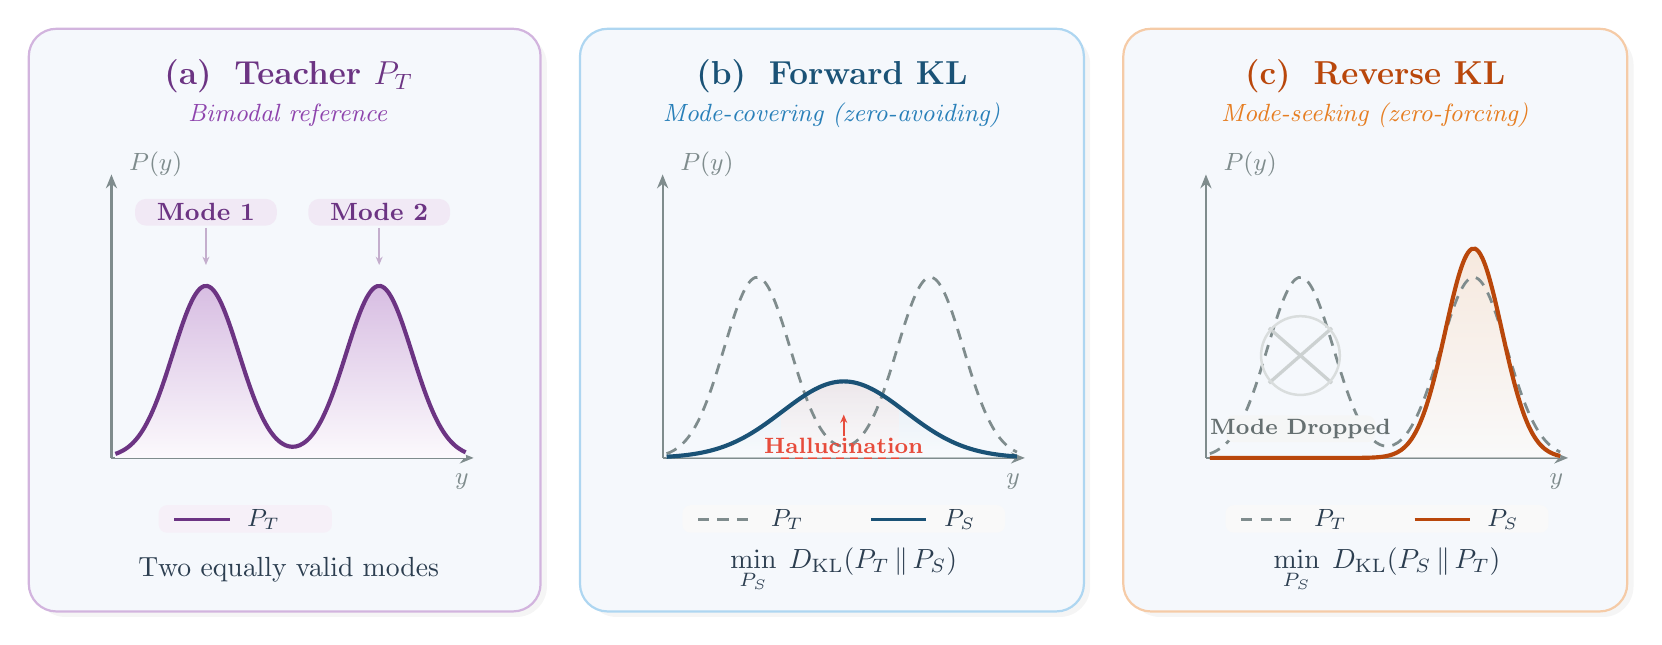
\begin{tikzpicture}[>=Stealth]

  % =================== Panel (a): Teacher P_T ===================
  \fill[black, opacity=0.04, rounded corners=11pt] (0.08, -1.87) rectangle (6.58, 5.53);
  \fill[panelbg, rounded corners=10pt] (0, -1.8) rectangle (6.5, 5.6);
  \draw[lightpurple, line width=0.8pt, rounded corners=10pt] (0, -1.8) rectangle (6.5, 5.6);

  \begin{scope}[shift={(1.05, 0.15)}]
    \node[font=\large\bfseries, deeppurple] at (2.25, 4.85) {(a)\; Teacher $P_T$};
    \node[font=\small, midpurple] at (2.25, 4.35) {\textit{Bimodal reference}};
    \draw[-{Stealth[length=5pt,width=4pt]}, line width=0.8pt, midgray]
      (0, 0) -- (4.6, 0);
    \node[font=\small, midgray, anchor=north] at (4.45, -0.08) {$y$};
    \draw[-{Stealth[length=5pt,width=4pt]}, line width=0.8pt, midgray]
      (0, 0) -- (0, 3.6);
    \node[font=\small, midgray, anchor=south west] at (0.1, 3.45) {$P(y)$};
    \shade[top color=midpurple!35, bottom color=midpurple!3, smooth, samples=100, domain=0.05:4.5]
      plot (\x, {2.3*(exp(-((\x-1.2)^2)/(2*0.42^2)) + exp(-((\x-3.4)^2)/(2*0.42^2)))/(0.42*sqrt(2*pi))})
      -- (4.5,0) -- (0.05,0) -- cycle;
    \draw[deeppurple, line width=1.5pt, smooth, samples=100, domain=0.05:4.5]
      plot (\x, {2.3*(exp(-((\x-1.2)^2)/(2*0.42^2)) + exp(-((\x-3.4)^2)/(2*0.42^2)))/(0.42*sqrt(2*pi))});
    \fill[midpurple!12, rounded corners=4pt] (0.3, 2.95) rectangle (2.1, 3.29);
    \node[font=\small\bfseries, deeppurple] at (1.2, 3.12) {Mode 1};
    \fill[midpurple!12, rounded corners=4pt] (2.5, 2.95) rectangle (4.3, 3.29);
    \node[font=\small\bfseries, deeppurple] at (3.4, 3.12) {Mode 2};
    \draw[-{Stealth[length=3pt,width=2.5pt]}, deeppurple!40, line width=0.6pt] (1.2, 2.92) -- (1.2, 2.45);
    \draw[-{Stealth[length=3pt,width=2.5pt]}, deeppurple!40, line width=0.6pt] (3.4, 2.92) -- (3.4, 2.45);
    \fill[midpurple!8, rounded corners=3pt] (0.6, -0.6) rectangle (2.8, -0.95);
    \draw[deeppurple, line width=0.9pt] (0.8, -0.78) -- (1.5, -0.78);
    \node[font=\small, deepgray, anchor=west] at (1.6, -0.78) {$P_T$};
    \node[font=\normalsize, deepgray] at (2.25, -1.42)
      {Two equally valid modes};
  \end{scope}

  % =================== Panel (b): Forward KL ===================
  \fill[black, opacity=0.04, rounded corners=11pt] (7.08, -1.87) rectangle (13.48, 5.53);
  \fill[panelbg, rounded corners=10pt] (7.0, -1.8) rectangle (13.4, 5.6);
  \draw[lightblue, line width=0.8pt, rounded corners=10pt] (7.0, -1.8) rectangle (13.4, 5.6);

  \begin{scope}[shift={(8.05, 0.15)}]
    \node[font=\large\bfseries, deepblue] at (2.15, 4.85) {(b)\; Forward KL};
    \node[font=\small, midblue] at (2.15, 4.35) {\textit{Mode-covering (zero-avoiding)}};
    \draw[-{Stealth[length=5pt,width=4pt]}, line width=0.8pt, midgray]
      (0, 0) -- (4.6, 0);
    \node[font=\small, midgray, anchor=north] at (4.45, -0.08) {$y$};
    \draw[-{Stealth[length=5pt,width=4pt]}, line width=0.8pt, midgray]
      (0, 0) -- (0, 3.6);
    \node[font=\small, midgray, anchor=south west] at (0.1, 3.45) {$P(y)$};
    \shade[top color=midblue!20, bottom color=midblue!2, opacity=0.5, smooth, samples=100, domain=0.05:4.5]
      plot (\x, {1.9*exp(-((\x-2.3)^2)/(2*0.78^2))/(0.78*sqrt(2*pi))})
      -- (4.5,0) -- (0.05,0) -- cycle;
    \draw[coralpink, line width=0.9pt, dash pattern=on 3pt off 2pt, smooth, samples=60, domain=1.5:3.0]
      plot (\x, {1.9*exp(-((\x-2.3)^2)/(2*0.78^2))/(0.78*sqrt(2*pi))});
    \draw[coralpink, line width=0.9pt, dash pattern=on 3pt off 2pt] (1.5, 0) -- (3.0, 0);
    \shade[top color=coralpink!18, bottom color=coralpink!2, opacity=0.4, smooth, samples=60, domain=1.5:3.0]
      plot (\x, {1.9*exp(-((\x-2.3)^2)/(2*0.78^2))/(0.78*sqrt(2*pi))})
      -- (3.0, 0) -- (1.5, 0) -- cycle;
    \draw[midgray, line width=1.0pt, dash pattern=on 4pt off 3pt, smooth, samples=100, domain=0.05:4.5]
      plot (\x, {2.3*(exp(-((\x-1.2)^2)/(2*0.42^2)) + exp(-((\x-3.4)^2)/(2*0.42^2)))/(0.40*sqrt(2*pi))});
    \draw[deepblue, line width=1.5pt, smooth, samples=100, domain=0.05:4.5]
      plot (\x, {1.9*exp(-((\x-2.3)^2)/(2*0.78^2))/(0.78*sqrt(2*pi))});
    \node[font=\footnotesize\bfseries, coralpink, inner sep=0pt] at (2.3, 0.15) {Hallucination};
    \draw[-{Stealth[length=3pt,width=2.5pt]}, coralpink, line width=0.7pt] (2.3, 0.28) -- (2.3, 0.55);
    \fill[midgray!5, rounded corners=3pt] (0.25, -0.6) rectangle (4.35, -0.95);
    \draw[midgray, line width=1.0pt, dash pattern=on 4pt off 3pt] (0.45, -0.78) -- (1.15, -0.78);
    \node[font=\small, deepgray, anchor=west] at (1.25, -0.78) {$P_T$};
    \draw[deepblue, line width=0.9pt] (2.65, -0.78) -- (3.35, -0.78);
    \node[font=\small, deepgray, anchor=west] at (3.45, -0.78) {$P_S$};
    \node[font=\normalsize, deepgray] at (2.3, -1.42)
      {$\displaystyle\min_{P_S}\; D_{\mathrm{KL}}(P_T \,\|\, P_S)$};
  \end{scope}

  % =================== Panel (c): Reverse KL ===================
  \fill[black, opacity=0.04, rounded corners=11pt] (13.98, -1.87) rectangle (20.38, 5.53);
  \fill[panelbg, rounded corners=10pt] (13.9, -1.8) rectangle (20.3, 5.6);
  \draw[lightorange, line width=0.8pt, rounded corners=10pt] (13.9, -1.8) rectangle (20.3, 5.6);

  \begin{scope}[shift={(14.95, 0.15)}]
    \node[font=\large\bfseries, deeporange] at (2.15, 4.85) {(c)\; Reverse KL};
    \node[font=\small, midorange] at (2.15, 4.35) {\textit{Mode-seeking (zero-forcing)}};
    \draw[-{Stealth[length=5pt,width=4pt]}, line width=0.8pt, midgray]
      (0, 0) -- (4.6, 0);
    \node[font=\small, midgray, anchor=north] at (4.45, -0.08) {$y$};
    \draw[-{Stealth[length=5pt,width=4pt]}, line width=0.8pt, midgray]
      (0, 0) -- (0, 3.6);
    \node[font=\small, midgray, anchor=south west] at (0.1, 3.45) {$P(y)$};
    \shade[top color=midorange!28, bottom color=midorange!3, opacity=0.5, smooth, samples=100, domain=0.05:4.5]
      plot (\x, {2.4*exp(-((\x-3.4)^2)/(2*0.36^2))/(0.36*sqrt(2*pi))})
      -- (4.5,0) -- (0.05,0) -- cycle;
    \draw[midgray, line width=1.0pt, dash pattern=on 4pt off 3pt, smooth, samples=100, domain=0.05:4.5]
      plot (\x, {2.3*(exp(-((\x-1.2)^2)/(2*0.42^2)) + exp(-((\x-3.4)^2)/(2*0.42^2)))/(0.40*sqrt(2*pi))});
    \draw[deeporange, line width=1.5pt, smooth, samples=100, domain=0.05:4.5]
      plot (\x, {2.4*exp(-((\x-3.4)^2)/(2*0.36^2))/(0.36*sqrt(2*pi))});
    \draw[midgray!40, line width=1.2pt] (0.8, 0.95) -- (1.6, 1.65);
    \draw[midgray!40, line width=1.2pt] (0.8, 1.65) -- (1.6, 0.95);
    \draw[midgray!30, line width=0.9pt] (1.2, 1.3) circle (0.5);
    \fill[midgray!8, rounded corners=3pt] (0.25, 0.2) rectangle (2.15, 0.54);
    \node[font=\footnotesize\bfseries, midgray!80!black] at (1.2, 0.37) {Mode Dropped};
    \fill[midgray!5, rounded corners=3pt] (0.25, -0.6) rectangle (4.35, -0.95);
    \draw[midgray, line width=1.0pt, dash pattern=on 4pt off 3pt] (0.45, -0.78) -- (1.15, -0.78);
    \node[font=\small, deepgray, anchor=west] at (1.25, -0.78) {$P_T$};
    \draw[deeporange, line width=0.9pt] (2.65, -0.78) -- (3.35, -0.78);
    \node[font=\small, deepgray, anchor=west] at (3.45, -0.78) {$P_S$};
    \node[font=\normalsize, deepgray] at (2.3, -1.42)
      {$\displaystyle\min_{P_S}\; D_{\mathrm{KL}}(P_S \,\|\, P_T)$};
  \end{scope}

\end{tikzpicture}
}
\caption{Forward KL vs.\ Reverse KL divergence for fitting a student distribution $P_S$ to a bimodal teacher $P_T$. \textbf{(a)}~The teacher places equal probability mass on two valid modes (e.g., two correct answers or two stylistic variants). \textbf{(b)}~Forward KL minimizes $\KL(P_T \parallel P_S)$ and is mode-covering (zero-avoiding): the student spreads a single broad Gaussian over both modes and places substantial probability in the inter-mode hallucination zone (red dashed boundary), corresponding to outputs that are a blend of the two valid answers and therefore neither. \textbf{(c)}~Reverse KL minimizes $\KL(P_S \parallel P_T)$ and is mode-seeking (zero-forcing): the student concentrates sharply onto a single peak (Mode 2), dropping Mode 1 entirely but producing crisp, coherent generations within the chosen mode. This trade-off motivates the adaptive-divergence methods in \S\ref{sec:objectives} (ToDi, AKL, Entropy-Aware OPD), which interpolate between the two regimes based on per-token teacher entropy or log-ratio statistics.}
\label{fig:kl_divergence}
\end{figure*}

DistiLLM-2's source-level adaptation represents a first step toward acknowledging that no single divergence is universally optimal, but it operates at a coarse granularity (entire sequences grouped by data source). The fixed-divergence family faces a deeper limitation rooted in the heterogeneity of autoregressive token distributions \emph{within} a single sequence. The choice between Forward KL (mode-covering) and Reverse KL (mode-seeking) is a global decision applied uniformly across all token positions (Figure~\ref{fig:kl_divergence}). Yet the teacher's distributional structure varies dramatically within a single sequence. At a mathematical operator token, the teacher concentrates probability mass on one or two correct symbols, making mode-seeking optimal because the student must commit to the correct answer. At a conjunction or filler word, dozens of tokens share comparable probability, making mode-covering optimal because any synonym suffices and the student should preserve this flexibility. Applying a single divergence to both positions necessarily compromises in a way that compounds across sequence length: Forward KL wastes gradient signal on high-entropy positions where any token is acceptable, while Reverse KL discards useful coverage information at low-entropy positions where multiple valid continuations exist. This is not merely an efficiency concern but a fundamental misalignment between the geometry of the loss and the geometry of the target distribution, motivating the per-position adaptation that follows.

Sequence-level objectives offer a complementary perspective. MiniLLM~\citep{2306.08543} elevates Reverse KL to the full sequence level, where the student $\ptheta$ appears inside the sampling expectation. The central challenge is computing the gradient of an expectation over $\ptheta$ when $\ptheta$ itself is parameterized by $\theta$. Starting from $\KL(\ptheta \parallel \pteacher) = \E_{y \sim \ptheta}[\log \ptheta(y|x) - \log \pteacher(y|x)]$ and applying the log-derivative trick:
\begin{equation}
    \nabla_\theta \loss_{\text{MiniLLM}} = \E_{y \sim \ptheta} \left[ \Big( \log \ptheta(y|x) - \log \pteacher(y|x) \Big) \nabla_\theta \log \ptheta(y|x) \right]
\end{equation}
Minimizing sequence-level Reverse KL is thus mathematically equivalent to policy gradient RL with reward $r(x,y) = \log \pteacher(y|x) - \log \ptheta(y|x)$. MiniLLM decomposes this into per-step rewards $r_t$ and future returns $R_t = \sum_{t'=t}^{|y|} r_{t'}$, enabling variance-reducing baselines:
\begin{equation}
    \nabla_\theta \loss_{\text{MiniLLM}} = -\E_{y \sim \ptheta} \left[ \sum_{t=1}^{|y|} \left( R_t - b \right) \nabla_\theta \log \ptheta(y_t|y_{<t}) \right]
\end{equation}
where $b$ is a learned baseline. The single-step decomposition is not merely an implementation convenience but serves a deeper purpose. By attributing credit to individual token decisions via $R_t$, MiniLLM enables the student to identify exactly which reasoning step caused a trajectory to diverge from the teacher, rather than assigning uniform blame across all tokens. This fine-grained credit assignment places optimization squarely in the RL framework, with the teacher's log-probability serving as a dense reward signal. The connection to policy optimization explains MiniLLM's strong performance on reasoning tasks where sequence-level coherence matters more than token-level accuracy. The cost is high because REINFORCE estimation in massive combinatorial output spaces demands substantially more training iterations and sophisticated baseline subtraction to converge. KETCHUP~\citep{2504.19024} directly targets this variance problem by replacing the single-sample REINFORCE estimator with a $K$-step truncated return, reducing gradient variance while preserving the sequence-level objective. The constrained KD framework of~\citet{2509.22921} further augments the sequence-level Reverse KL with a hard KL constraint implemented via state-augmented CMDP, ensuring that the student's divergence from the teacher remains bounded even during aggressive exploration.

\textbf{The token-level vs.\ sequence-level tradeoff.} The choice between token-level and sequence-level objectives represents a core bias-variance tradeoff whose resolution foreshadows the RL-augmented methods of \S\ref{subsec:rl_objectives}. Token-level methods (GKD, DistiLLM) provide $|V|$-dimensional gradient signals at every position, yielding low variance but potentially biased gradients when the teacher's token-level distribution is poorly calibrated (the flawed prefix trap of Section~\ref{subsec:weighting}). Sequence-level methods (MiniLLM, KETCHUP) provide unbiased gradients through the policy gradient theorem but suffer from high variance due to single-sample REINFORCE estimation over exponentially large sequence spaces. The practical resolution is task-dependent. For instruction following where token-level teacher quality is high, GKD-style methods dominate. For reasoning tasks where sequence-level coherence is paramount, MiniLLM-style methods are preferred despite their variance, and KETCHUP's truncated returns offer an intermediate point on this spectrum. Recognizing that MiniLLM is already performing policy gradient RL (with the teacher's log-probability as reward) clarifies that sequence-level distillation and RL-augmented distillation are not distinct paradigms but endpoints of a continuum parameterized by the reward source: pure teacher signal at one end, pure task reward at the other, and hybrid objectives (G-OPD, RLKD) interpolating between them.

\textbf{Full-vocabulary vs.\ sampled-token KL.} Orthogonal to the token-level vs.\ sequence-level choice, a practical implementation decision determines how much of the teacher's distribution is used at each position. Many RL-based OPD implementations approximate the per-position KL by computing $\log \pi_\theta(y_t|y_{<t}) - \log \pi_T(y_t|y_{<t})$ only at the \emph{sampled} token $y_t$, treating this scalar as a per-token advantage within a policy gradient framework~\citep{lu2025onpolicy}. While computationally lightweight (requiring only one teacher log-probability per position), this single-sample estimate introduces high gradient variance and discards the distributional information across non-sampled tokens. DeepSeek-V4~\citep{deepseekv4} shows that \emph{full-vocabulary} logit distillation, computing the exact $\KL(\ptheta(\cdot|y_{<t}) \parallel \pteacher(\cdot|y_{<t}))$ over all $|V|$ tokens at each position, yields substantially more stable gradients and more faithful knowledge transfer at the cost of transmitting or reconstructing the full teacher logit vector. Their engineering solution (caching teacher hidden states and reconstructing logits on-the-fly through the prediction head) makes this feasible even with 10+ trillion-parameter teachers over vocabularies exceeding 100K tokens, establishing full-vocabulary KL as the preferred choice for industrial-scale OPD when infrastructure permits. Lightning OPD~\citep{wu2026lightning} further establishes that the full teacher forward pass can be entirely eliminated by precomputing teacher log-probabilities over SFT rollouts, achieving 4$\times$ speedup over standard OPD under a \emph{teacher consistency} condition (using the same teacher for both SFT data generation and distillation).

\subsection{Adaptive Divergence Objectives}
\label{subsec:adaptive_div}

Adaptive methods address this per-position mismatch by selecting or interpolating divergences based on local distributional geometry. When the teacher is certain (low entropy), mode-seeking Reverse KL preserves precision, and when uncertain (high entropy), mode-covering Forward KL preserves diversity.

ToDi~\citep{2505.16297} implements this insight through per-token weighting derived from the teacher-student probability log-ratio. A sigmoid-based function $w_t = \sigma(\log p_T(y_t|y_{<t}) - \log p_\theta(y_t|y_{<t}))$ dynamically blends Forward KL and Reverse KL for each token:
\begin{equation}
    \loss_{\text{ToDi}} = \E_{y \sim \ptheta} \left[ \sum_{t=1}^{|y|} w_t \cdot \KL(\pteacher \parallel \ptheta) + (1-w_t) \cdot \KL(\ptheta \parallel \pteacher) \right]
\end{equation}
where $w_t$ emphasizes Forward KL for tokens the student underestimates (boosting their probability) and Reverse KL for tokens it overestimates (suppressing excess probability). Entropy-Aware OPD~\citep{2603.07079} takes an alternative approach, using the teacher's per-token entropy $H(\pteacher(\cdot|y_{<t}))$ as a gating signal. The base objective is Reverse KL at all positions, with Forward KL \emph{additively} activated at high-entropy tokens where the teacher distributes probability across multiple valid continuations:
\begin{equation}
    \loss_{\text{EA}} = \E_{y \sim \ptheta} \left[ \sum_{t=1}^{|y|} \KL(\ptheta \parallel \pteacher) + \mathbb{I}[H_t > \tau] \cdot \KL(\pteacher \parallel \ptheta) \right]
\end{equation}
Both methods consistently outperform any fixed divergence on math reasoning (MATH, GSM8K) and open-ended generation (AlpacaEval), confirming that the optimal divergence is indeed position-dependent. The complementarity between these two methods is instructive. ToDi conditions adaptation on the teacher-student gap (a pairwise property), while Entropy-Aware OPD conditions on teacher uncertainty alone (a marginal property). The former adapts more aggressively when the student is far from the teacher, while the latter provides a stable routing signal independent of student quality, making it more suitable for early training when the student's distribution is unreliable.

AKL~\citep{2404.02657} synthesizes elements of both approaches, dynamically interpolating between Forward KL and Reverse KL based on a per-token confidence metric derived from the teacher-student probability ratio. Unlike entropy-based routing, which depends only on the teacher's distributional shape, AKL considers the \emph{relative} geometry of teacher and student, adapting more aggressively at positions where the gap is largest. All three adaptive methods admit a natural interpretation through information geometry. The Fisher information metric on the statistical manifold of autoregressive distributions varies across token positions. At reasoning-critical positions, the manifold is highly curved (the teacher concentrates probability on few tokens), making Reverse KL's mode-seeking behavior locally appropriate because it follows the manifold's natural gradient. At generation-flexible positions, the manifold is nearly flat (many synonyms are equally valid), and Forward KL's mode-covering behavior preserves useful entropy. Adaptive divergences implicitly navigate this varying curvature by selecting the locally optimal metric, which explains their consistent empirical superiority over any fixed choice.

The field has thus moved decisively from ``which divergence?'' to ``which divergence \emph{where}?'' The evidence from ToDi, AKL, and Entropy-Aware OPD converges on a consistent finding across evaluated settings, that no single fixed divergence dominates uniformly, and even the simplest adaptive routing (a hard entropy threshold) outperforms the best-tuned fixed alternative. Yet adaptive divergences, however sophisticated their per-token routing, share a fundamental limitation with their fixed counterparts. They optimize a distance to the teacher distribution. Perfect optimization under any $f$-divergence yields a student that matches the teacher but never exceeds it. When the teacher itself makes errors or lacks reasoning paths that a well-guided student could discover, divergence minimization becomes a ceiling rather than a floor.

\subsection{RL-Augmented Objectives}
\label{subsec:rl_objectives}

Divergence matching, whether fixed or adaptive, intrinsically limits the student to the teacher's capability ceiling. Perfect optimization yields a student that matches (but never exceeds) the teacher's distribution. RL-augmented objectives break this ceiling by introducing an external performance signal that can steer the student toward solutions the teacher would never produce.

\textbf{OPD as KL-constrained RL.} G-OPD~\citep{2602.12125} establishes a formal equivalence between standard OPD and dense KL-constrained reinforcement learning. It formulates distillation as maximizing a token-level reward derived from teacher logits, penalized by divergence from a reference policy:
\begin{equation}
    \max_\theta \E_{y \sim \ptheta} \left[ \sum_{t=1}^{|y|} \alpha \log \pteacher(y_t | y_{<t}) - \KL\big(\ptheta(\cdot | y_{<t}) \parallel p_{\text{ref}}(\cdot | y_{<t})\big) \right]
\end{equation}
When $\alpha = 1$, this reduces to standard Reverse KL distillation. When $\alpha > 1$, the objective forces the student to \emph{extrapolate} beyond the teacher's probability mass, enabling a phenomenon documented as \emph{Reward Extrapolation}, whereby the student discovers previously unseen, structurally sound reasoning paths in regions where the teacher's generation probability $\pteacher(y|x)$ is low but the outcome reward remains high. In the multi-teacher setting where several domain-specific RL experts share the same base model, reward extrapolation (ExOPD) produces a unified student that surpasses all its same-size domain teachers, demonstrating that OPD need not be a lossy compression step.

This equivalence has a deeper theoretical consequence that unifies the entire section. It bridges the distillation and RL communities by showing that all objectives discussed here (GKD's token-level KL, MiniLLM's sequence-level Reverse KL, G-OPD's reward-augmented formulation) are special cases of KL-constrained policy optimization with different reward definitions and constraint strengths. Any advance in KL-constrained RL (better trust regions, adaptive penalty coefficients, variance reduction) immediately transfers to OPD, and vice versa.

\textbf{Gradient decomposition and the KD+RL complementarity.} The unified KD+RL framework of~\citet{2512.23097} decomposes the hybrid gradient into two orthogonal components, a dense KD gradient for token-level imitation and a Monte Carlo RL gradient for reward maximization. The KD component dampens the high variance inherent in policy gradient estimation, while the RL component prevents the student from collapsing onto teacher modes that are suboptimal for the downstream task. REOPOLD~\citep{2603.11137} instantiates this insight by interpreting on-policy distillation as policy optimization where the teacher-student log-likelihood ratio acts as a token reward. It stabilizes training through three mechanisms: mixture-based reward clipping to prevent over-trust of extreme teacher signals, entropy-based dynamic sampling to selectively leverage teacher feedback at high-uncertainty tokens, and a unified exploration-to-refinement schedule. Empirically, REOPOLD achieves 6.7--12$\times$ greater sample efficiency than recent RL approaches and enables a 7B student to match a 32B teacher in visual reasoning with $\sim$3.3$\times$ inference speedup.

\textbf{Structure-aware reward as an alternative to dense KL.} While G-OPD and REOPOLD retain token-level KL as the primary distillation signal (differing only in how they augment or stabilize it), RLKD~\citep{2505.16142} departs from this template entirely by replacing token-level KL with a Generative Structure Reward Model (GSRM). The GSRM parses both teacher and student reasoning paths into sequences of meta-reasoning and solving steps, then scores structural alignment between the two sequences. This structural reward is combined with a task-level outcome reward (e.g., math accuracy) and optimized via GRPO:
\begin{equation}
    R_{\text{total}}(x, y) = \alpha \, R_{\text{GSRM}}(y, y^{\text{teach}}) + (1-\alpha) \, R_{\text{outcome}}(x, y)
\end{equation}
The key insight is that reasoning distillation need not operate at the token level. By supervising at the \emph{step structure} level, RLKD avoids the vocabulary-coupling assumption of logit-based methods while still transferring the teacher's multi-branch reasoning strategy. Empirically, RLKD trained on only 0.1\% of the data under a pure RL regime surpasses standard SFT-RL pipelines, demonstrating that structural reward can substitute for dense KL when the teacher's value lies in its reasoning organization rather than its token-level distribution. This progression from dense token-level KL (G-OPD) through variance-reduced token rewards (REOPOLD) to step-level structural matching (RLKD) traces an increasing abstraction of what ``teacher knowledge'' means, moving from distributional fidelity to behavioral organization.

\textbf{Joint vs.\ sequential optimization.} Given that KD and RL provide complementary gradient signals (dense imitation vs.\ sparse reward maximization), a persistent engineering challenge is \emph{how} to combine them within a single training pipeline without mutual interference. Sequential approaches (distill-then-RL or RL-then-distill) suffer from catastrophic interference, as the RL stage erases distilled knowledge through policy drift, while the KD stage suppresses previously unseen solutions discovered through exploration. KDRL~\citep{2506.02208} implements joint optimization by adding an on-policy KL regularizer between student and teacher \emph{during} RL training, preventing policy drift while still allowing reward-driven exploration. RLAD~\citep{2602.22495} refines this further by recognizing that unconditional KL regularization is itself suboptimal. Its Trust Region Ratio Distillation (TRRD) replaces the standard KL penalty with a PPO-style likelihood-ratio objective anchored to a teacher-old-policy mixture. This selective strategy follows the teacher only when its signal improves the policy update, preventing blind KL minimization from dragging the student toward suboptimal trajectories on problems the teacher itself cannot solve. The progression from KDRL's uniform regularization to RLAD's selective trust region mirrors the fixed-to-adaptive evolution in divergence objectives (Section~\ref{subsec:fixed_div}$\to$\ref{subsec:adaptive_div}), confirming a recurring principle across this survey, that conditioning the learning signal on local geometry outperforms uniform application.

\textbf{Preference-based objectives as implicit RL.} When logit access is unavailable or when sequence-level quality judgments are more natural than token-level distributions, several methods map the KD+RL problem onto Direct Preference Optimization (DPO). AlignDistil~\citep{2503.02832} constructs synthetic preference pairs from student rollouts scored by the teacher, applying both standard and reverse DPO objectives. OVD~\citep{2601.21968} queries the teacher for pairwise preferences over student-generated responses, avoiding continuous probability extraction entirely. These preference-based objectives share a fundamental connection to token-level KL methods. Under DPO's closed-form solution, the optimal policy satisfies $\pi^*(y|x) \propto \pi_{\text{ref}}(y|x) \exp(r(y,x)/\beta)$, and substituting the teacher's log-probability as the implicit reward yields the geometric mixture distribution targeted by GKD with $\lambda$-mixing. The practical implication is that DPO-style methods are most useful when constructing preference pairs is cheaper than computing full teacher logits. PBSD~\citep{pbsd2026} pushes this connection further in the self-distillation regime by deriving the reward-regularized optimum $\pi^* \propto \pi_{\text{teach}} \exp(r/\beta)$ against a context-augmented teacher rather than a static reference policy, and showing that the resulting pairwise preference loss provably dominates direct KL matching when the reward signal is informative (Section~\ref{subsec:self_pi}). The landscape exposes a unifying gradient. Token-level KL (G-OPD, REOPOLD), step-level structure matching (RLKD), and sequence-level preference ranking (AlignDistil, OVD) all implement KL-constrained policy optimization at different abstraction levels, with the appropriate level determined by signal availability and the granularity at which teacher expertise manifests.

\textbf{Fine-grained credit assignment.} All methods above, whether operating at the token, step, or sequence level, share one limitation: they apply supervision uniformly across the student's trajectory. When the student makes a single error in step 3 of a 10-step proof, wholesale imitation retrains all 10 steps, diluting the corrective gradient on the actual failure point. SuperCorrect~\citep{2410.09008} introduces hierarchical thought templates with cross-model DPO for error localization, identifying which reasoning step diverged and concentrating feedback there. SCoRe~\citep{2509.14257} pushes targeting to its logical extreme, correcting \emph{only the earliest error} in the student's trajectory, concentrating all supervision at the single point of maximum leverage. This exploits the cascading nature of reasoning errors, where correcting the root cause eliminates all downstream consequences simultaneously. The contrast with RLKD's structural approach is instructive. RLKD rewards trajectories whose overall step organization matches the teacher's, while SCoRe surgically corrects the first point of divergence. The two are complementary, and combining global structural reward with local error correction remains unexplored.

\textbf{From signal matching to environment reconstruction.} The most radical extension asks whether the student can recover the teacher's \emph{underlying optimization landscape}. $\mathcal{X}$-KD~\citep{2602.12674} adopts the AVRIL framework to jointly model the teacher's latent reward function and perform policy distillation, encouraging the student to optimize in a reconstructed version of the teacher's training environment rather than mimicking its outputs. TSD-KD~\citep{2603.13260} combines indirect distillation (student generates candidates that the teacher re-ranks via preference feedback) with direct distillation (KL matching applied selectively to high-entropy tokens where teacher-student gaps are largest). These methods represent the current frontier, moving from matching the teacher's \emph{behavior} to understanding its \emph{incentives}.

Across objective types, a clear hierarchy emerges. Fixed divergences provide stable, well-understood optimization but are limited by the teacher's capability ceiling. Adaptive divergences improve efficiency by matching the local geometry of the loss landscape. RL-augmented objectives break through the ceiling entirely but introduce variance and instability. The optimal choice depends on the specific application. For instruction following where teacher quality is high, fixed or adaptive divergences suffice. For reasoning tasks where the student must exceed the teacher, RL augmentation is essential. For tasks where the teacher's training process is accessible, environment reconstruction offers the most complete knowledge transfer.

\section{Signal Source and Teacher Architecture}
\label{sec:signal}

With the objective function fixed (Section~\ref{sec:objectives}), the practitioner must determine \emph{where the teacher signal comes from}, whether through full logit access (white-box), API-only text outputs (black-box), or the model's own internal asymmetries (self-distillation). Each signal source imposes distinct constraints on the applicable objectives and achievable performance.

Historically, signal sources have evolved in step with model access constraints. Early OPD methods (GKD, DistiLLM) assumed full white-box access to model internals, a requirement that limits distillation to same-organization deployments. The rise of proprietary API-only models (GPT-4, Claude) necessitated black-box methods that can extract knowledge from text outputs alone. Most recently, self-distillation methods eliminate the external teacher entirely, enabling continuous improvement without access to any stronger model. This progression from full access through limited access to no external access represents increasing autonomy at the cost of signal density, a core trade-off that shapes every downstream design decision.

Complex reasoning is where OPD proves most indispensable and where off-policy methods encounter their hardest limits. The reason is structural, because reasoning is \emph{path-dependent}~\citep{2306.13649}. A proof that begins ``assume for contradiction...'' requires entirely different subsequent tokens than one beginning ``we proceed by induction...'' If the student has never generated the inductive approach during training, it cannot recover at inference time when that path would be optimal. Off-policy training over a fixed dataset of teacher reasoning traces can only cover a finite set of solution paths, while the student needs to navigate its own unique landscape of partial solutions, dead ends, and recovery strategies. This insight motivates the on-policy formulation for reasoning transfer. The student generates its own intermediate reasoning steps $r^S \sim P_\theta(\cdot|x)$, and the teacher evaluates these student-generated chains rather than dictating its own:
\begin{equation}
    \loss_{\text{CoT-OPD}}(\theta) = \E_{x \sim \mathcal{D},\; r^S \sim P_\theta(\cdot|x)} \left[ \sum_{t=1}^{|r^S|} \KL\!\left( P_T(\cdot|x, r^S_{<t}) \;\|\; P_\theta(\cdot|x, r^S_{<t}) \right) \right]
\end{equation}
The Forward KL direction ensures mode-covering, meaning the student must allocate probability wherever the teacher does on the student's own prefixes, effectively receiving corrective feedback on its actual generation patterns rather than memorizing the teacher's preferred trajectories. This self-consistent learning dynamic, where the student practices its own reasoning style under expert supervision, has made on-policy CoT distillation the de facto paradigm for transferring multi-step reasoning to smaller models. The principle that rationale transfer outperforms answer-only supervision was first established in the off-policy setting by~\citet{2305.02301}, and subsequent work demonstrated that generating rationales on-policy~\citep{2306.13649} yields further gains by eliminating exposure bias, a finding validated at scale by DeepSeek-R1~\citep{2501.12948} and its successors.

\subsection{White-Box Logit Supervision}
\label{subsec:white_box}

White-box access provides the densest possible signal, namely the full probability distribution across $|V|$ tokens at every decoding step. This exposes the teacher's implicit decision boundaries, including the relative probabilities among incorrect tokens (Hinton's ``dark knowledge''), which carry information about similarity structure that binary labels cannot capture.

\textbf{Standard logit distillation.} The majority of methods surveyed in Section~\ref{sec:objectives} assume white-box access. GKD, DistiLLM, ToDi, G-OPD, and their variants all require computing $\pteacher(\cdot|x, y_{<t})$ at each student-generated token position. The computational cost is dominated by the teacher forward pass, executed once per student-generated token (or once per sequence when caching is enabled).

\textbf{Token-level adaptive supervision.} Within the white-box setting, several methods refine \emph{which} tokens receive supervision, and they can be organized along the axis of what drives the selection decision. SelecTKD~\citep{2510.24021} routes based on student-teacher agreement, applying a propose-and-verify mechanism where the student proposes tokens that the teacher verifies, and only positions where agreement holds receive full loss while rejected tokens are masked or down-weighted. AdaSwitch~\citep{2510.07842} routes based on student prefix reliability, maintaining a running error estimate and switching between exploration (student generates freely) and guidance (teacher provides dense supervision) so that guidance kicks in only when the trajectory has drifted far enough to warrant teacher intervention. Token-Adaptive KD~\citep{2510.11615} routes based on gradient magnitude, computing per-token importance weights from the KL loss itself and concentrating compute where the teacher-student gap is largest. The three selection criteria, agreement, prefix quality, and gradient magnitude, are complementary rather than competing, each capturing a different signal about where supervision is most informative. They also compose naturally with entropy-based divergence routing (ToDi, Entropy-Aware), which selects \emph{which loss function} applies at each position while token-level selection determines \emph{how much gradient signal} propagates. The combination yields an orthogonal two-dimensional design space that current methods have only begun to explore jointly. These token-selection mechanisms complement the sample-level and token-level weighting schemes discussed in Section~\ref{sec:dynamics}.

The temporal scope of white-box distillation is not limited to post-training. MiniPLM~\citep{2410.17215} extends on-policy distillation to the \emph{pre-training} stage, showing that distilling during pre-training yields stronger foundations for downstream fine-tuning. This represents a qualitative shift, because rather than being a post-hoc compression step, OPD becomes an integral part of the model creation pipeline. Gemma~2~\citep{2408.00118} validates this approach at industrial scale, embedding KD directly into the pre-training loop for its 27B$\to$9B$\to$2B model cascade. The success of pre-training distillation raises a deeper question, namely whether OPD should be viewed as a separate post-processing step at all, or as an intrinsic component of the training objective alongside next-token prediction.

A critical challenge arises when teacher and student use different tokenizers or vocabulary sizes. Direct KL divergence over mismatched vocabularies is undefined. DSKD~\citep{2504.11426} solves this through \emph{dual-space} knowledge distillation, introducing projectors that map between teacher and student representation spaces:
\begin{equation}
    \mathcal{L}_{\text{DSKD}} = \KL(P_{T \to S} \parallel P_S) + \KL(P_{S \to T} \parallel P_T)
\end{equation}
where $P_{T \to S}$ denotes the teacher's hidden states projected into the student's space and decoded through the student's prediction head. An exact token alignment algorithm handles vocabulary mismatches by identifying identical tokens across tokenizers. Vocabulary tokens with similar semantic embeddings should receive similar probability mass even when the tokenization schemes differ, enabling distillation across different architectures (e.g., Llama teacher to Qwen student) that share no vocabulary overlap.

Cross-Tokenizer KD~\citep{2402.12030} takes a complementary approach based on optimal transport, computing an alignment matrix between teacher and student token sequences that minimizes the earth mover's distance in latent space:
\begin{equation}
    \mathcal{L}_{\text{CrossTok}} = \inf_{\pi \in \Pi(P_S, P_T)} \E_{(z_S, z_T) \sim \pi} \left[ \| W_{S \to T} z_S - z_T \|_2^2 \right]
\end{equation}
The distinction between hidden-state alignment (DSKD) and vocabulary-space alignment (Cross-Tokenizer KD) exposes a fundamental design trade-off. Hidden-state alignment preserves richer representational structure but requires maintaining two projectors during training. Vocabulary-space alignment is more lightweight but operates at a level where information has already been compressed through the vocabulary bottleneck. In either case, the alignment maps must be \emph{co-trained} with the student because the student's representation space shifts during on-policy training as its policy evolves, a form of representation drift absent in off-policy settings. Concrete Score Matching~\citep{2509.25837} provides yet another solution, distilling via a continuous score function that bypasses the discrete vocabulary mismatch entirely. Together, these methods make OPD architecture-agnostic, allowing organizations to distill from any available teacher (e.g., Llama-based) into any student architecture (e.g., Qwen-based) without the historically restrictive requirement of shared vocabulary, enabling heterogeneous teacher-student pairs that were previously infeasible.

Beyond selecting \emph{which tokens} to supervise, a complementary question is \emph{what information} the teacher should provide at each token. Not all content in the teacher's logits is equally useful. Delta-KD~\citep{2509.14526} introduces the principle of \emph{signal isolation}, distilling only the differential shift between a base model and its instruction-tuned variant. Since the base model's distribution captures generic language modeling knowledge the student already possesses through pre-training, distilling it is redundant at best and harmful at worst because it wastes gradient budget on information the student has already internalized. By extracting only the instruction-following delta, Delta-KD provides a cleaner supervisory signal that transfers alignment without overwriting the student's foundation.

A related but distinct challenge is teacher \emph{overconfidence}. When the teacher assigns extreme probability to tokens outside the student's reachable space, the resulting optimization targets are simultaneously precise and useless. Two complementary solutions address this from opposite directions. Veto~\citep{2601.07155} (Adaptive Target Reformulation) refines the teacher's output \emph{post-hoc}, constructing a geometric bridge in logit space with a parameter $\beta$ that serves as both an Adaptive Gradient Veto (suppressing pathological gradients on low-confidence tokens) and a Decisiveness Knob (balancing performance with diversity), dynamically reformulating the teacher's target distribution based on the student's current capability. PromptKD~\citep{2402.12842} takes the opposite approach, adapting the teacher \emph{pre-hoc} by prepending learnable prompt tokens (adding only 0.0007\% of the teacher's parameters) that cause the teacher to produce ``student-friendly'' distributions more accessible to the student's limited capacity. The distinction is instructive. Post-hoc methods (Veto, Delta-KD) operate on the supervisory signal after it is produced, while pre-hoc methods (PromptKD) modify the teacher's generation process itself. Both are effective, and their composition is orthogonal.

TAID~\citep{2501.16937} introduces yet another dimension of adaptation, namely temporal interpolation of the target itself. It constructs a time-dependent intermediate distribution $P_t = (1-\lambda_t) P_\theta + \lambda_t P_T$ that starts close to the student and progressively approaches the full teacher distribution as training proceeds. This temporal curriculum over the target (rather than over the input prompts as in PACED) provides a complementary axis of control. PACED asks ``which problems to train on,'' while TAID asks ``how much of the teacher's knowledge to reveal at each stage.'' The progression from PACED (problem-level curriculum) through AdaSwitch (token-level timing) to TAID (target-level interpolation) and PromptKD (teacher-level adaptation) traces an important design spectrum, showing that curriculum can operate at four distinct granularities (prompt, token, target, teacher), all of which address the same underlying bottleneck of keeping the difficulty gap between teacher signal and student capability in the productive learning range. Because these four granularities are orthogonal, they can be combined within a single training loop, and systems that integrate all four should achieve the most efficient distillation.

\subsection{Black-Box and API-Constrained Distillation}
\label{subsec:black_box}

When only API access is available, the student observes the teacher's top-1 text output (or at best, top-$k$ log-probabilities) rather than the full distribution. This information bottleneck eliminates token-level divergence matching and forces methods to operate at the sequence level. Despite this limitation, black-box methods have proven surprisingly effective, suggesting that much of the teacher's knowledge is recoverable from text-only observations.

\textbf{Distilling Step-by-Step.} \citet{2305.02301} demonstrated the foundational black-box approach, extracting not just the teacher's final answers but its intermediate reasoning steps (rationales) as additional supervision. Although technically off-policy (the student fine-tunes on static teacher-generated rationales rather than its own), this work is the conceptual ancestor of on-policy CoT distillation and established a key principle. The student is trained with a multi-task objective combining answer prediction and rationale generation, enabling a 770M-parameter model to outperform a 540B-parameter teacher with 500$\times$ fewer parameters and substantially less training data (50\% fewer examples on average, up to 85\% reduction on some tasks). This demonstrated that \emph{how} the teacher reasons is often more valuable than \emph{what} it concludes, a principle that pervades modern OPD and motivates the on-policy extensions below.

If extracting textual rationales recovers partial teacher reasoning, the natural next question is whether a richer proxy for the teacher's full distribution can be reconstructed from black-box outputs alone. The following methods attempt progressively more aggressive reconstructions, from adversarial discrimination through verbal scoring to preference ranking.

\textbf{Adversarial distribution matching.} GAD~\citep{2511.10643} reformulates the distillation problem as a generative adversarial game:
\begin{equation}
    \max_{G} \min_{D}\; V(G, D) = \E_{(x, y^T) \sim \mathcal{T}} \left[ -\log \sigma\!\left( D(y^T) - D(G(x)) \right) \right]
\end{equation}
A discriminator $D$ (initialized from the student with a scalar prediction head) distinguishes student rollouts from teacher API outputs via a Bradley-Terry preference model, while the generator $G$ maximizes $V$ via REINFORCE using the discriminator score as an evolving on-policy reward signal. Unlike white-box methods that match full distributions, GAD extracts knowledge through a scalar quality signal, trading distributional fidelity for API compatibility. It inherits the training instability of adversarial objectives, as the discriminator can overfit to stylistic cues rather than semantic quality, but yields consistent gains over SFT baselines.

\textbf{Verbal feedback and curriculum.} Lion~\citep{2305.12870} exploits the teacher's capacity as a natural language critic through a three-stage adversarial loop. First, in \emph{imitation}, the student is fine-tuned on teacher-generated responses. Second, in \emph{discrimination}, the teacher identifies instructions on which the student still falls short. Third, in \emph{generation}, the teacher creates harder instructions targeting the student's identified weaknesses. This closed-loop curriculum progressively narrows the teacher-student gap without requiring any gradient information from the teacher, making it applicable to any instruction-following API. Lion-13B achieves competitive performance on BIG-Bench Hard and AGIEval using only 70K training examples.

\textbf{Didactic-to-constructive learning.} DAIL~\citep{2602.02405} addresses the gap between high-quality expert solutions (often out-of-distribution) and the student's actual reasoning space. Fine-tuning on expert solutions yields poor transfer because the student never learns to navigate its own reasoning space. DAIL uses a two-step process, transforming expert solutions into detailed, in-distribution reasoning traces via mixed policy decoding (the student generates while conditioned on the ground-truth solution), and applying a contrastive objective to focus learning on expert methodologies rather than surface patterns. Using fewer than 1,000 expert solutions, DAIL achieves 10--25\% pass@k gains, confirming the recurrent principle that the alignment of the supervision signal with the student's current distribution matters more than its absolute quality.

Distribution-Aligned Sequence Distillation (DASD)~\citep{2601.09088} reexamines the dominant practice of SFT on teacher-generated reasoning traces, identifying three limitations. First, inadequate representation of the teacher's sequence-level distribution from single best-of-$n$ samples. Second, misalignment between teacher output distribution and student capacity. Third, exposure bias from teacher-forced training. Its distribution-aligned pipeline addresses all three by generating multiple diverse teacher traces per prompt and aligning the student's generation distribution with the teacher's through sequence-level matching, achieving state-of-the-art performance using only 448K training samples. DDT~\citep{2602.12222} complements DASD's empirical findings with a theoretical framework explaining why RL generalizes better than SFT for reasoning. RL's on-policy data generation keeps training aligned with the model's evolving distribution rather than a static snapshot.

\textbf{Verbal score distillation.} OVD~\citep{2601.21968} replaces token-level probability matching entirely with trajectory matching using discrete verbal scores (0--9) from teacher models. This eliminates the requirement for token-level alignment between vocabularies, dramatically reduces memory consumption by avoiding logit storage, and delivers up to +12.9\% absolute EM improvement on web QA and +25.7\% on math benchmarks with a single rollout sample. The surprising effectiveness of such coarse supervision indicates that on-policy exploration itself provides a substantial fraction of the learning signal, with the teacher's role being more to \emph{select among student trajectories} than to \emph{correct individual tokens}.

These methods form a spectrum of signal richness versus access requirements. Adversarial methods recover the densest proxy for the teacher's distribution but require the most complex training dynamics (discriminator co-training, generator-discriminator instability). Score-based methods are simpler to train but lose distributional information, recovering only a scalar quality signal. Preference-based methods occupy a principled middle ground, recovering relative quality without requiring calibrated absolute scores, and their connection to DPO-style objectives provides well-understood convergence guarantees. Practitioners should therefore select the signal type matching their API access tier, with full logit access leading to KL methods (Section~\ref{sec:objectives}), unavailable token-level logits pointing to adversarial or score-based approaches, and ranking-only access favoring preference-based methods.

\textbf{Preference-based formulations.} ORPO-Distill~\citep{2509.25100} maps black-box distillation onto preference optimization, generating candidate responses from the student and querying the teacher API for pairwise rankings. The mixed-policy strategy, combining on-policy student traces with off-policy teacher traces, outperforms both pure off-policy and pure on-policy alternatives, suggesting that the contrastive structure of preference learning (learning what \emph{not} to do alongside what to do) provides complementary signal to the positive-only feedback of score-based methods. ThinkTuning~\citep{rrv2025thinktuning} occupies an intermediate position between black-box distillation and RL. Rather than providing scores after the fact, a same-size teacher reviews the student's incorrect answers \emph{during} the GRPO training loop and provides short corrective hints (rather than complete solutions). This interleaving of corrective feedback episodes with RL training acts as an implicit privileged signal that shapes policy gradient updates and is particularly effective for base models that lack strong prior reasoning behaviors, achieving +3.85\% over zero-shot baselines across benchmarks (+2.08\% on MATH-500, +2.23\% on AIME, +3.99\% on GPQA-Diamond over vanilla GRPO).

\textbf{MoE discriminator for pipeline-staged OPD.} PRISM~\citep{wang2026prism} introduces a distinct architectural innovation to black-box distillation by inserting an OPD-based \emph{pre-alignment} stage between SFT and RLVR, addressing the observation that direct RLVR from SFT checkpoints suffers from cold-start instability due to the large distributional gap between SFT outputs and reward-aligned behavior. Rather than using a monolithic discriminator (as in GAD), PRISM employs a Mixture-of-Experts discriminator with specialized perception and reasoning expert heads, providing \emph{disentangled} corrective signals that distinguish visual grounding errors from logical reasoning failures. The adversarial game operates entirely at the response level without requiring teacher logits. The student generates on-policy responses, a black-box teacher (Gemini 3 Flash) provides reference demonstrations, and the MoE discriminator learns to distinguish them while providing differentiated feedback through its expert routing. This disentangled feedback is critical for multimodal models where failure modes are heterogeneous, since a model may correctly perceive an image but reason incorrectly about it, or vice versa. On Qwen3-VL at 4B and 8B scales, the pre-alignment stage alone yields +4.4 and +6.0 points over direct SFT-to-RLVR pipelines, and the subsequent RLVR training converges faster and more stably, suggesting that black-box OPD provides a structured warm-up that shapes the policy landscape for downstream RL optimization.

\textbf{Off-policy knowledge integration.} Not all training signal must originate on-policy. Incorporating knowledge from off-policy sources (e.g., pre-existing teacher-generated datasets) into an on-policy framework presents its own difficulties. LUFFY~\citep{2504.14945} addresses this by extending GRPO to a mixed-policy objective that incorporates off-policy reasoning traces alongside the student's on-policy rollouts. The key design challenge is preventing \emph{superficial imitation}, because without correction the student tends to copy high-probability tokens from off-policy traces while ignoring low-probability but critical reasoning steps. LUFFY's policy shaping via regularized importance sampling reweights gradients to emphasize learning from unfamiliar yet effective actions, achieving +6.4 average points over standard RLVR.

\subsection{Self-Distillation}
\label{subsec:self_distill}

Self-distillation eliminates the need for an external teacher entirely. Instead, the model exploits asymmetries \emph{within itself} to construct a training signal. Three families of methods have emerged, distinguished by the source of this internal asymmetry, namely privileged information that is available at training but not inference time, self-play between successive model checkpoints, and external feedback from verifiers or environments that the model itself has generated.

\subsubsection{Privileged Information}
\label{subsec:self_pi}

The first family creates asymmetry through \emph{privileged information} (PI), meaning training-time access to context unavailable at inference. Conditioning the same model on additional context produces a strictly stronger policy that can supervise the unconditioned version, turning a single network into both teacher and student.

\textbf{Ground-truth as PI.} OPSD~\citep{2601.18734} constructs the teacher policy by conditioning on both the problem $x$ and the ground-truth answer $y^\star$, while the student conditions only on $x$. The student generates on-policy rollouts, and the teacher provides dense token-level supervision.
\begin{equation}
    \loss_{\text{OPSD}}(\theta) = \E_{(x, y^\star) \sim \mathcal{S}} \E_{\hat{y} \sim \ptheta(\cdot|x)} \left[ \sum_{n=1}^{|\hat{y}|} D\!\left( p_\theta(\cdot|x, y^\star, \hat{y}_{<n}) \;\|\; \ptheta(\cdot|x, \hat{y}_{<n}) \right) \right]
\end{equation}
On competition-level math benchmarks (AIME 2024/2025, HMMT), OPSD matches or exceeds GRPO at 4B and 8B scales while using only a single rollout per problem versus GRPO's eight, achieving a significant computational advantage. At 1.7B scale, however, the gains over GRPO are minimal, indicating that sufficient model capacity is necessary for the PI mechanism to provide useful supervision. The teacher's ground-truth conditioning must produce meaningfully different token distributions from the student, which requires enough parameters to represent the conditional shift.

A complementary limitation arises when all rollouts for a given prompt fail (the ``cliff prompt'' problem), causing the policy gradient to vanish entirely. This failure mode directly parallels PACED's finding (Section~\ref{subsec:weighting}) that gradient SNR vanishes when student pass rate approaches zero, but with an important difference. PACED addresses this through curriculum selection (avoiding problematic prompts), while HDPO~\citep{2603.23871} addresses it through signal augmentation. HDPO augments GRPO with a JSD-based self-distillation term on ground-truth-conditioned rollouts, ensuring non-zero gradients even at the boundary of the student's competence, directly patching the cliff-prompt vulnerability without restricting the problem distribution.

\textbf{Relaxing the ground-truth requirement.} Ground-truth labels are not always available. GATES~\citep{2602.20574} demonstrates that \emph{any} training-time context can serve as PI by having a single model act as tutor (conditioned on a source document) and student (answering from the question alone). Because source documents do not guarantee correct answers, GATES introduces a consensus-based gating mechanism that suppresses the gradient when tutor uncertainty is high, preventing the model from reinforcing unreliable self-supervision.~\citet{2602.04942} generalize the OPSD and GATES paradigms into a unified theoretical framework, formalizing the conditions under which privileged self-distillation provably improves over standard training.

\textbf{Behavioral PI: context distillation.} The PI paradigm extends beyond factual ground truth to behavioral instructions. OPCD~\citep{2602.12275} treats system prompts, exemplars, and retrieval context as privileged information, enabling a model to internalize behaviors that would otherwise require expensive in-context demonstrations at inference time. OPSDL~\citep{2604.17535} extends this to long-context settings, applying on-policy self-distillation to enhance long-context capabilities without relying on high-quality supervision data or sparse sequence-level rewards and enabling stable optimization for context lengths beyond what standard post-training methods achieve. OEL~\citep{2603.16856} extends to continuous post-deployment learning, using interaction outcomes as dynamic PI that updates the model's teacher policy as it accumulates experience, closing a loop that OPCD opened.

\textbf{Reasoning compression via PI.} CRISP~\citep{2603.05433} finds that a model prompted to ``be concise'' can serve as a teacher for its own verbose version, reducing chain-of-thought token count by 57--59\% on MATH-500 while \emph{improving} accuracy by 9--16 percentage points. Much of the verbosity in distilled reasoning models is trainable inefficiency rather than a necessary feature of competent reasoning.

\textbf{Visual PI for GUI grounding.} GUI-SD~\citep{zhang2026guisd} extends the privileged information paradigm to multimodal GUI grounding, where the task is to predict click coordinates on a screen given a natural language instruction. The privileged context is a Gaussian soft mask centered on the target element's bounding box, providing the teacher version with explicit spatial localization that the student must learn to infer from raw screenshots alone. This represents a qualitatively different form of PI from textual ground truth (OPSD) or document context (GATES), one that is \emph{visual} and \emph{spatial}, demonstrating that the PI mechanism generalizes across modalities. Beyond the new PI type, GUI-SD introduces entropy-guided token weighting via a dual-criterion, where tokens receive higher loss weight based on both their digit significance (coordinate digits carry more semantic weight than filler tokens) and the teacher's confidence at that position. With only a single on-policy rollout per instance, GUI-SD outperforms GRPO (which requires multiple rollouts for reward estimation) on six GUI grounding benchmarks including ScreenSpot-v2, ScreenSpot-Pro, and OSWorld. The success of single-rollout PI distillation in the visual domain mirrors OPSD's finding in mathematical reasoning, providing further evidence that privileged information provides sufficiently dense gradient signal to obviate the sample-intensive reward estimation required by RL-based alternatives.

\textbf{Cross-lingual safety via PI.} MSD~\citep{qin2026msd} extends the PI paradigm to multilingual safety alignment, where the same model's English-language reasoning serves as privileged information for its low-resource-language student, transferring safety boundaries without target-language safety data. Its Dual-Perspective Safety Weighting (DPSW) concentrates distillation gradients on safety-critical tokens by combining teacher confidence with student disagreement. We discuss MSD's broader implications for safety-aware OPD in Section~\ref{sec:future}.

\textbf{Beyond KL matching via reward regularization.} A recurring concern across the PI literature above is that directly matching the privileged teacher's distribution can destabilize training and, in the worst case, degrade reasoning capability as training proceeds. PBSD~\citep{pbsd2026} diagnoses this pathology through a reward-regularized lens, replacing pure KL matching with the objective $\max_{\pi} \E[r(x,y)] - \beta D_{\mathrm{KL}}(\pi \,\|\, \pi_{\text{teach}})$, whose analytic optimum is a reward-reweighted teacher $\pi^* \propto \pi_{\text{teach}}(y|x) \exp(r(x,y)/\beta)$ that provably dominates the teacher itself whenever the reward is informative. Practically, PBSD realizes this optimum through a DPO-style pairwise loss where the preferred sample $y^+$ is drawn from the context-augmented teacher and the dispreferred sample $y^-$ from the current student, preserving on-policy sampling while avoiding the forced imitation of every teacher token. On Qwen3-1.7B/4B/8B, PBSD is the only self-distillation method that both matches OPSD's token efficiency and surpasses its peak accuracy without the post-peak decline documented in Figure~2 of~\citet{pbsd2026}, suggesting that preference-based targets are a more principled substitute for direct KL matching than curriculum or signal-augmentation patches alone. This post-peak decline is the same pathology that CaOPD~\citep{2604.16830} attributes to the training-deployment context mismatch and that~\citet{2603.24472} diagnose as epistemic suppression (Section~\ref{subsec:failure}), so PBSD can also be read as a self-distillation mechanism that converts these diagnostic insights into a corrective optimization target rather than a post-hoc recalibration step.

\textbf{Outcome-conditioned PI at the turn level for agentic reasoning.} The PI methods above all target single-turn generation. Extending PI to multi-turn agentic settings raises a distinct question, namely at which temporal granularity should privileged information intervene? Existing agentic OPD work has explored the \emph{trajectory} granularity (TCOD's temporal curriculum over turn prefixes, Section~\ref{subsec:curriculum}), the \emph{step} granularity (MAD-OPD's step-level decomposition, Section~\ref{sec:applications}), and the \emph{skill} granularity (Skill-SD's skill-conditioned updates, Section~\ref{sec:applications}), but none of them supply PI at the \emph{turn} level itself. TT-OPD~\citep{ttopd2026} fills this gap. A gradient-free EMA teacher receives correctness-dependent cues (reinforcing phrases for trajectories scored correct, corrective phrases for those scored incorrect) that are inserted at the prompt-response boundary and then stripped from the teacher's output log-probabilities, so the student never observes the hints directly but still receives an outcome-aware KL signal at every conversation turn. Two aspects distinguish this instance from prior PI mechanisms. \emph{First, the privileged context encodes trajectory-level correctness rather than problem-level ground truth}, which is the first PI realization we are aware of where the teacher is conditioned on a property of the student's own rollout rather than on external supervision. This generalizes the PI paradigm from single-response supervision (GATES, OPSD, GUI-SD) to multi-turn behavioral regularization. \emph{Second, the ablation isolates why turn-level PI is necessary}: EMA teacher updates alone eliminate the KL-collapse pathology but still allow the multi-turn structure to erode, and outcome hints without length control trigger response explosion, so neither EMA nor hints in isolation suffice. These pathologies are precisely the failure modes documented in Section~\ref{subsec:failure}, and the interaction between teacher dynamics and outcome-conditioned PI is what makes agentic OPD stable.

Viewed together with TCOD, Skill-SD, and MAD-OPD, TT-OPD completes a granularity spectrum for agentic distillation in which the choice of temporal unit (trajectory, turn, step, skill) is matched to the level at which errors compound in the target task.

\subsubsection{Self-Play}
\label{subsec:self_play}

A more radical question is whether a model can improve using nothing but its own rollouts, with no PI, no external feedback, and no additional context. The answer is a qualified yes, subject to important saturation limitations.

\textbf{Self-play as a two-player game.} SPIN~\citep{2401.01335} casts self-improvement as an adversarial game between successive checkpoints, training the updated model to distinguish its previous iteration's generations from human-written responses:
\begin{equation}
    \loss_{\text{SPIN}} = \E_{x, y \sim p_{\text{data}}, y' \sim p_{\theta_t}} \left[ \ell\!\left( \lambda\left(\log \frac{p_{\theta_{t+1}}(y|x)}{p_{\theta_t}(y|x)} - \log \frac{p_{\theta_{t+1}}(y'|x)}{p_{\theta_t}(y'|x)}\right) \right) \right]
\end{equation}
SPIN provides a theoretical convergence guarantee. The global optimum of $\loss_{\text{SPIN}}$ is achieved if and only if $p_{\theta_{t+1}} = p_{\text{data}}$, i.e., the student's distribution exactly matches the reference distribution. At this fixed point, the loss is zero and the gradient vanishes, so the iterative process is \emph{stable}. Once the student reaches the target distribution, further iterations cannot destabilize it. The game-theoretic interpretation is that $p_{\text{data}}$ is the unique Nash equilibrium of the two-player game, and SPIN's iterative updates correspond to fictitious play converging to this equilibrium. Starting from Zephyr-7B-SFT, it improves MT-Bench from 5.94 to 6.78 over 3 iterations, with diminishing returns at each round. This convergence guarantee comes with an inherent limitation: SPIN converges to $p_{\text{data}}$, not to the optimal policy. If the reference data is sub-optimal (as human-written responses often are), SPIN will faithfully reproduce those sub-optimalities, confirming that pure self-play recycles existing knowledge rather than generating new knowledge.

IRIS~\citep{2604.20933} provides a unifying framework for this family by replacing the implicit KL divergence in SPIN with an interpolative R\'{e}nyi divergence parameterized by $\alpha \in (0, \infty)$, recovering SPIN ($\alpha \to 1$, KL regime), SPACE (Jensen-Shannon regime), and SPIF ($\alpha = 2$, $\chi^2$-regularized regime) as special cases. The R\'{e}nyi parameter controls the exploration-exploitation tradeoff, with lower $\alpha$ encouraging broader distributional coverage (exploration) while higher $\alpha$ concentrates updates on the most likely improvements (exploitation). This unification shows that the various self-play methods in the literature differ only in their implicit divergence choice, not in their fundamental mechanism, and suggests that $\alpha$-tuning can be used as a meta-parameter for adapting self-play behavior to task requirements.

The trajectory from SPIN through IRIS to $\pi$-Play traces an escalating response to the saturation ceiling. SPIN accepts the ceiling (converging to $p_{\text{data}}$). IRIS pushes the ceiling by tuning the divergence's exploration-exploitation balance via the R\'{e}nyi parameter. $\pi$-Play shatters the ceiling by introducing internal privileged information that generates genuinely new training signal. Each step demonstrates that self-play is not inherently limited, but that breaking saturation requires progressively more creative sources of asymmetry. When internal asymmetry is exhausted, the only remaining option is to inject external ground truth, motivating the external grounding mechanisms of Section~\ref{subsec:external_feedback}.

\textbf{Beyond adversarial games.} The self-play paradigm extends beyond explicit two-player games to encompass several lighter-weight mechanisms. SDFT~\citep{2601.19897} positions on-policy self-distillation as a mechanism for forgetting resistance via implicit KL regularization against the model's own prior checkpoint, converting the model's optimization trajectory into a regularization resource for continual learning. MTP via self-distillation~\citep{2602.06019} targets \emph{architectural} rather than behavioral improvement, converting a pre-trained autoregressive model into a multi-token predictor by training an auxiliary prediction head on the model's own next-token predictions, achieving $>3\times$ faster decoding at typically 3--7\% accuracy drop (model-dependent) and expanding the scope of what self-distillation can optimize.

On-Policy SFT~\citep{zhao2026onpolicy} provides a surprising simplification. By filtering self-generated responses for correctness (via a verifier) and conciseness (via length truncation at the median successful length), standard SFT on this filtered on-policy data matches or exceeds full RL training. The combination of on-policy generation (which naturally produces diverse solution strategies) with outcome filtering (which selects the best strategies) implicitly performs a form of evolutionary optimization that requires no gradient through the reward function. This ``generate-filter-train'' paradigm dramatically reduces implementation complexity compared to full RL-based distillation while retaining the core benefit of on-policy data, namely distributional alignment. Self-Distilled RLVR~\citep{yang2026selfdistilled} further decomposes the gradient update into two components. Self-distillation determines the \emph{magnitude} of per-token policy updates (how much to change each token's probability), while environmental RLVR feedback anchors the \emph{direction} (which tokens should increase vs.\ decrease). At just 200 training steps, RLSD surpasses GRPO trained for 400 steps on Qwen3-VL-8B-Instruct, demonstrating 2$\times$ sample efficiency from the complementary signal structure.

\textbf{Minimalist self-distillation.} SSD~\citep{zhang2026embarrassingly} requires no RL, no verifier, no external teacher, and no code execution. It samples solutions at training-time temperature, fine-tunes via standard SFT, and reshapes token distributions in a context-dependent manner. On LiveCodeBench v6, SSD improves Qwen3-30B-Instruct from 42.4\% to 55.3\%, demonstrating that when the base model is sufficiently capable, even the simplest self-play yields substantial gains. The requirement is not a sophisticated algorithm but sufficient \emph{diversity} in the model's sampling distribution to produce high-quality variants that can serve as training targets.

Yet this also exposes the fundamental boundary of pure self-play. When diversity is achieved through temperature sampling alone, the model's improvement is ultimately bounded by the information already present in its pre-training distribution. Bridging this boundary requires either connecting the model to external reality (Section~\ref{subsec:external_feedback}) or internally generating privileged information through the self-play process itself ($\pi$-Play below).

\textbf{Unifying PI and self-play.} $\pi$-Play~\citep{zhang2026piplay} unifies privileged information and self-play within a single multi-agent self-evolution framework. Self-play naturally produces a byproduct during task generation, the examiner agent constructs a question construction path (QCP) that provides high-quality PI at no additional cost. Three co-evolving agents (examiner $\pi^E_\phi$, teacher $\pi^T_\psi$ conditioned on QCP, student $\pi^S_\theta$ without it) are jointly optimized through alternating updates. As the student strengthens, the examiner generates harder tasks, and the teacher's behavior is softly constrained to track the student via a KL penalty, establishing a self-adjusting curriculum that requires no external data. On Qwen3 (4B, 8B), data-free $\pi$-Play surpasses fully supervised search agents such as Search-R1 and delivers substantially higher evolutionary efficiency than conventional self-play (Dr.Zero), with the largest gains on multi-hop benchmarks where the teacher's token-level credit assignment provides the most leverage.

\textbf{Partial-solution PI.} PAINT~\citep{wang2026paint} occupies a distinctive position between pure self-play (no external information) and full PI (complete answer revealed). Rather than conditioning on the entire ground-truth solution (as in OPSD), PAINT reveals only a \emph{partial} solution whose extent is adaptively controlled by the overlap between the student's rollout and the reference. It computes a recall-style overlap score based on the fraction of reference anchors (boxed answers, formulas, key numbers) that appear in the student's rollout, revealing more of the reference when the student is close (providing fine-grained correction) and less when far (preventing trivial copying). This overlap-adaptive partial-solution masking creates a natural curriculum within the PI mechanism itself, where easy problems where the student nearly solves them receive precise corrective feedback, while hard problems where the student diverges completely receive only coarse directional guidance. PAINT further introduces energy-space interpolation that applies the distillation loss only at positions where the teacher-student entropy mismatch exceeds a threshold, producing a sparse loss that concentrates gradient signal on the most informative positions. On competition-level mathematics (AIME 2024/2025 and HMMT 2025 average), PAINT achieves +2.1 over the OPSD baseline and +2.9 over GRPO, demonstrating that partial revelation of privileged information can outperform both full revelation and no revelation, suggesting an optimal information disclosure curve that future work should characterize theoretically.

Together, $\pi$-Play and PAINT demonstrate that the self-play saturation problem can be mitigated \emph{without} external feedback by internally generating privileged information, whether through multi-agent task construction or partial-solution conditioning. This mechanism is orthogonal to the external-verification strategies below, and combining both internal PI and external grounding remains an unexplored direction.

\subsubsection{External Feedback}
\label{subsec:external_feedback}

The self-play methods above require no external input but face an inherent ceiling. Without ground-truth or verifier access, the model cannot distinguish confident-but-wrong outputs from genuinely correct ones, leading to the saturation problem analyzed in Section~\ref{subsec:failure}. External feedback methods retain the self-distillation architecture (no separate teacher model) while injecting non-differentiable truth signals, typically code execution, symbolic verification, or outcome rewards, that anchor the self-play loop and prevent it from collapsing onto self-reinforcing errors. Unlike the internal-PI mechanisms of $\pi$-Play and PAINT, external feedback bridges self-distillation and reinforcement learning by treating environmental signals as the ultimate arbiter when internal asymmetries are exhausted.

\textbf{From binary rewards to dense supervision.} SD-ZERO~\citep{he2026selfdistillation} converts sparse verifier signals into dense self-supervision through a dual-role architecture. The Generator produces on-policy responses while the Reviser, conditioned on the Generator's output and its binary correctness signal, produces an improved version. The Generator then distills from the Reviser's token-level distribution, converting binary feedback into dense self-supervision. On Qwen3-4B-Instruct, SD-ZERO achieves 68.3\% on AIME 2024, outperforming GRPO (62.5\%), demonstrating that self-revision can be more effective than standard RL for converting sparse rewards into learning signal. SDPO~\citep{2601.20802} extends this beyond binary feedback to \emph{structured textual} feedback, including runtime errors, failing unit tests, and LLM judge evaluations that construct fine-grained credit assignment attributing success or failure to specific reasoning steps rather than entire trajectories. RL from Text Feedback (RLTF)~\citep{song2026expanding} pushes further with free-form natural language critiques from an automated judge, training the model's single-turn policy to match its own feedback-conditioned second-turn generations.

From SD-ZERO's binary signal through SDPO's structured errors to RLTF's free-form critiques, a clear trajectory emerges. As external feedback becomes richer, the self-distillation objective becomes more precisely targeted, enabling the model to correct specific failure modes rather than globally adjusting its policy. Sample-Routed Policy Optimization (SRPO)~\citep{li2026unifying} shows that these approaches can be composed by routing. Correct samples follow GRPO's reinforcement path (reward-weighted likelihood maximization) while failed samples follow SDPO's targeted logit-level correction. The insight is that correct and incorrect samples carry distinct types of learning signal, and treating both identically wastes the information each carries. SRPO raises the five-benchmark average on Qwen3-8B by 3.4\% over GRPO and 6.3\% over SDPO alone across science and tool-use tasks, confirming that the optimal external-feedback strategy is a routing function matching each sample to its most informative objective.

\textbf{Environmental grounding.} RLTF and related methods use compiler outputs, unit test results, and symbolic math verifiers as external feedback that shatters self-reinforcing echo chambers. Even if the model becomes highly confident in a flawed derivation, the verifier assigns $R=0$, providing an unambiguous correction signal unavailable to pure self-play.

\textbf{Saturation analysis.} \citet{2603.24472} trace self-distillation degradation in mathematical reasoning to the suppression of \emph{epistemic verbalization}, the model's expression of uncertainty during reasoning. When self-distillation shortens reasoning traces, it disproportionately removes hedging phrases and uncertainty markers that serve as implicit ``attention flags'' for difficult sub-problems. The result is shorter but less calibrated reasoning, where the model confidently commits to flawed steps. This connects to the teacher uncertainty challenge in Section~\ref{sec:understanding}, where an overconfident student produces unreliable self-play targets, and the saturation problem ultimately requires either external grounding or the internally generated PI mechanism of $\pi$-Play to overcome.

Across signal sources, from white-box logits through black-box APIs to self-distillation, a fundamental trade-off between signal density and autonomy governs the design space. White-box methods provide the richest supervision ($|V|$-dimensional distributions at every token) but require same-organization deployment and co-location of teacher and student. Black-box methods sacrifice distributional information but operate across organizational boundaries, with recent methods (GAD, OVD) recovering surprisingly effective proxy signals. Self-distillation eliminates external dependencies entirely but is bounded by the model's pre-existing capabilities unless augmented by external verification or internally generated PI. This continuum is not merely descriptive but predictive, indicating where future methods will have the most impact. The white-box extreme is well-explored (GKD, DistiLLM, DSKD are mature), while the self-distillation extreme still lacks principled convergence guarantees for complex reasoning. The greatest innovation potential lies at the boundaries, in methods like ThinkTuning that blur the line between black-box feedback and RL, or methods like $\pi$-Play that blur the line between self-play and externally grounded verification.

\section{Training Dynamics and Efficiency}
\label{sec:dynamics}

Given an objective function (Section~\ref{sec:objectives}) and a signal source (Section~\ref{sec:signal}), the final engineering decision is \emph{how to stabilize and accelerate the on-policy training loop}. On-policy generation introduces unique optimization challenges absent from standard supervised fine-tuning, including non-stationary data distributions (the student's policy shifts during training, making older rollouts stale), gradient signal-to-noise ratio (SNR) collapse on hard prompts (where all rollouts fail and no useful gradient emerges), and the computational overhead of autoregressive student rollouts followed by teacher scoring (several times more expensive than off-policy training).

These challenges are not independent. SNR collapse on hard prompts wastes compute, motivating curriculum strategies that avoid such prompts. Non-stationarity invalidates cached teacher signals, motivating efficient online scoring. And the compute overhead of autoregressive generation creates a systems-level bottleneck that requires architectural solutions. The methods in this section address these challenges through three complementary mechanisms.

\subsection{Token and Sample Weighting}
\label{subsec:weighting}

Not all teacher supervision is equally reliable in the on-policy setting. The core problem is the \emph{flawed prefix trap}, where a student generating an erroneous token early in a sequence causes all subsequent teacher predictions to be conditioned on this out-of-distribution prefix. Because the teacher has never been trained on such prefixes, its conditional distribution $\pteacher(\cdot|x, \hat{y}_{<t}^{\text{bad}})$ becomes noisy and unreliable. Naively matching this corrupted signal propagates errors rather than correcting them.

\textbf{Teacher reliability filtering.} TIP~\citep{xu2026tip} (Token Importance Profiling) provides a principled framework for token weighting by organizing importance along two axes, student entropy $h_t$ and teacher-student divergence $\delta_t$. Crossing these axes yields four quadrants with qualitatively distinct learning roles. High-entropy, high-divergence tokens (Q1) carry the dominant corrective signal, high-entropy, low-divergence tokens (Q2) indicate agreement on uncertainty, low-entropy, high-divergence tokens (Q3) represent \emph{overconfident errors} where the student is certain but wrong, and low-entropy, low-divergence tokens (Q4) are genuinely mastered. The theoretical result shows that Q3 tokens are structurally invisible to any entropy-only weighting scheme, because no non-decreasing function of entropy with $f(0)=0$ can distinguish them from Q4. TIP's parameter-free Soft-OR score $s_t = \hat{h}_t + \hat{\delta}_t - \hat{h}_t \cdot \hat{\delta}_t$ recovers Q3 coverage while preserving Q1/Q2 sensitivity, achieving consistent improvements at 50\% token retention across three model families with capacity gaps from $2\times$ to $9\times$.

SCOPE~\citep{zheng2026scope} elevates this analysis from tokens to \emph{rollouts}. Its dual-path architecture routes rollouts by correctness. Incorrect trajectories receive teacher-perplexity-weighted KL distillation (down-weighting unreliable guidance on flawed prefixes), while correct trajectories receive student-perplexity-weighted MLE (concentrating reinforcement at the capability boundary). This addresses diversity collapse, the counterintuitive phenomenon where Pass@1 improves at the expense of Pass@$k$, yielding +7.3\% Pass@32 improvement over competitive baselines across six reasoning benchmarks.

SelecTKD~\citep{2510.24021} applies a propose-and-verify mechanism at the token level, where the student proposes tokens that the teacher verifies through greedy Top-k or non-greedy Spec-k matching. Accepted tokens receive full loss while rejected tokens are masked or down-weighted, inducing an implicit curriculum quantified by Token Acceptance Rate (TAR). Positions where teacher-student agreement fails indicate either genuine ambiguity or distributional divergence, and in neither case does the unfiltered gradient carry reliable information.

AdaSwitch~\citep{2510.07842} introduces a dynamic switching mechanism between pure exploration and guided distillation. Unlike static filtering that simply attenuates unreliable signals, AdaSwitch maintains a sliding window of recent token-level divergences (KL or JSD between student and teacher logits) and computes a running average $\bar{d}_i = \frac{1}{L}\sum_{j=i-L}^{i-1} d_j$ over a window of length $L$. When the current token's divergence exceeds a context-adaptive threshold $\tau_i = K \cdot \bar{d}_{i-1}$ (where $K$ is a sensitivity multiplier), the method switches from on-policy exploration to off-policy teacher guidance. This single-switch design preserves semantic coherence (avoiding the jarring token-level alternation of prior mixing methods) while ensuring high-quality supervision precisely when the student's generation drifts into high-divergence regions. The threshold's adaptive nature is essential, as a fixed threshold would be either too aggressive (switching on easy prefixes where minor divergence is harmless) or too permissive (failing to intervene when the student enters genuinely problematic states). By conditioning on recent divergence history, AdaSwitch calibrates its intervention threshold to the local sequence difficulty.

These four methods span a design spectrum from fine-grained to coarse-grained intervention. TIP applies continuous weighting over every token, SCOPE routes entire rollouts into distinct loss pathways, SelecTKD makes binary accept/reject decisions per token, and AdaSwitch commits to a single trajectory-level mode switch. The progression exposes an underlying tradeoff between signal fidelity (finer granularity preserves more information) and optimization stability (coarser decisions reduce gradient variance). This tradeoff is not merely theoretical. Fine-grained methods like TIP require reliable token-level teacher signals, which degrade precisely when the flawed prefix problem is severe. Coarse-grained methods sacrifice per-token optimality but are robust to local signal corruption because a single bad token cannot contaminate the entire trajectory's gradient. Practitioners can select along this spectrum based on the dominant failure mode in their setting. Token-level methods excel when teacher reliability varies sharply within a sequence (e.g., long reasoning chains where some steps are easy and others require critical insight), while trajectory-level methods are preferred when the primary concern is prefix-quality drift across the generation (e.g., multi-turn dialogue where early errors shift the entire conversation topic).

\textbf{Sample-level weighting.} Beyond token-level filtering, several methods weight entire samples based on their informativeness. The flawed prefix trap manifests most severely on \emph{hard} prompts where the student's pass rate approaches zero. On these prompts, nearly all rollouts contain early catastrophic errors, and the resulting teacher signals are dominated by noise. Methods that uniformly sample prompts waste most of their gradient budget on uninformative hard prompts or trivially correct easy prompts, with the productive learning concentrated on prompts at the boundary of the student's competence.

\textbf{Failure-mode analysis.} \citet{2603.25562} provide a systematic empirical analysis of why sampled-token OPD is fragile in long-horizon settings. They identify three failure modes: (1) an imbalanced one-token signal that reduces distribution matching to a single sample, (2) unreliable teacher guidance on student-generated prefixes that deviate from the teacher's training distribution, and (3) distortions caused by tokenizer or special-token mismatch. Their proposed fix, teacher top-$K$ local support matching via truncated Reverse KL with top-$p$ rollout sampling and special-token masking, yields more stable optimization across math reasoning and agentic training.

The token and sample weighting methods above operate \emph{reactively}, attenuating the loss signal \emph{after} the student has already generated a potentially uninformative rollout. A more proactive approach asks whether we can select prompts \emph{before} generation to maximize the expected information gain per rollout, motivating the curriculum methods below.

\subsection{Curriculum and Difficulty Adaptation}
\label{subsec:curriculum}

The sample weighting problem motivates a more principled solution. \emph{Curriculum design} actively selects prompts matching the student's current competence level. Where weighting operates on the loss \emph{after} generation, curriculum design intervenes \emph{before} generation by choosing which prompts to present. The design space spans multiple axes, including prompt difficulty, temporal depth within multi-turn interactions, semantic granularity of supervision, and initialization strategy, with each axis addressing a distinct failure mode of naive uniform sampling.

\textbf{Competence-boundary sampling.} PACED~\citep{2603.11178} models prompt difficulty dynamically using a Beta-kernel distribution centered on the student's current pass rate. The curriculum progressively shifts toward harder prompts as the student improves, while avoiding prompts where the pass rate is near zero (where gradient SNR vanishes) or near one (where the student has already mastered the content). This ``frontier sampling'' strategy concentrates the gradient budget on the narrow band of prompts where learning is most efficient.

The mathematical justification connects to the gradient SNR analysis. For a prompt with pass rate $p$, the expected gradient magnitude under binary reward vanishes at both extremes ($p \to 0$ and $p \to 1$) and peaks at intermediate difficulty. PACED formalizes this through a general Beta-kernel weight family $w(p) = p^\alpha(1-p)^\beta$, where the symmetric case $\alpha = \beta = 1$ yields the familiar $p(1-p)$ with peak at $p=0.5$, but asymmetric choices ($\alpha \neq \beta$) shift the peak to prioritize harder or easier prompts depending on the training phase. This generalization matters in practice because the optimal curriculum is rarely symmetric, as early training benefits from emphasizing moderate-difficulty prompts ($\alpha > \beta$, peak shifted left) while late training benefits from focusing on the remaining hard cases ($\alpha < \beta$). Concretely, PACED maintains a running estimate of per-prompt difficulty $\hat{p}_i$ (computed from the last $m$ rollouts) and samples each prompt with probability proportional to $\text{Beta}(\hat{p}_i; \alpha, \beta)$ where $(\alpha, \beta)$ control both the width and asymmetry of the competence frontier. Early in training, wide kernels cast a broad net. As training converges, narrow kernels focus on the diminishing frontier of unsolved problems. This concentrates rollouts on problems in the productive learning range and reduces wasteful sampling on already-mastered or intractable problems, translating directly into compute savings proportional to the curriculum efficiency.

This SNR analysis has a deeper implication that extends beyond curriculum design, as it explains \emph{why} on-policy training naturally outperforms off-policy on reasoning tasks without explicit curriculum engineering. In off-policy settings, the problem difficulty distribution is fixed by the dataset. As the student improves, an increasing fraction of training data falls into the ``too easy'' zone where gradients are negligible, leading to diminishing returns. On-policy training, by contrast, automatically adjusts the effective difficulty because the student's rollouts reflect its current capabilities, naturally generating sequences at the boundary of its competence. PACED makes this automatic adjustment explicit and optimal, but even naive on-policy training captures much of the benefit simply by sampling from $\ptheta$ rather than $\pdata$.

\textbf{Self-adjusting curricula.} Several methods from earlier sections provide implicit curriculum mechanisms without explicit difficulty estimation. $\pi$-Play's multi-agent framework (Section~\ref{subsec:self_play}) automatically generates harder tasks as the student strengthens, PAINT~\citep{wang2026paint} (Section~\ref{subsec:self_play}) adapts its partial-solution disclosure based on student-teacher overlap, and PRISM~\citep{wang2026prism} (Section~\ref{subsec:black_box}) shapes the policy landscape for subsequent RL through a structured multimodal warm-up. These complement PACED's explicit difficulty estimation with emergent difficulty adaptation.

\textbf{Dual-perspective curriculum.} Where PACED treats the student as a black box whose pass rate fully characterizes prompt difficulty, Uni-OPD~\citep{hou2026uniopd} argues that pass rate alone conflates two distinct failure modes: problems the student cannot solve (low pass rate due to capability gaps) and problems the student solves incorrectly in subtle ways (moderate pass rate but low-quality solutions). Separating these requires examining not just \emph{whether} the student succeeds but \emph{how} it fails. From the \emph{student} perspective, Uni-OPD implements difficulty-aware and correctness-aware data balancing that promotes exploration of informative states during rollout sampling, extending PACED's frontier-sampling insight from a single pass-rate metric to a dual-criterion that jointly considers problem difficulty and rollout correctness. From the \emph{teacher} perspective, it addresses a subtler failure mode. Even when the student generates informative rollouts, aggregated token-level supervision can become inconsistent with outcome-level reward signals. A trajectory that receives higher token-level teacher scores may actually produce a worse final answer. Uni-OPD's outcome-guided margin calibration restores order consistency between correct and incorrect trajectories, ensuring that the token-level gradient direction aligns with the sequence-level quality ordering. This dual-perspective framework generalizes across LLMs and MLLMs (5 domains, 16 benchmarks) and accommodates both single-teacher and multi-teacher settings, suggesting that the curriculum and supervision reliability problems are largely orthogonal and can be solved independently.

\textbf{Temporal curriculum for multi-turn distillation.} PACED, Uni-OPD, and the self-adjusting methods all operate along the \emph{difficulty} axis, selecting \emph{which prompts} to train on. TCOD~\citep{chen2026tcod} opens an orthogonal axis by asking not which prompts but \emph{how deep} within a single prompt's trajectory to apply supervision, addressing a failure mode unique to multi-turn agent distillation. In standard OPD applied to multi-turn tasks, the student generates entire interaction trajectories and receives teacher supervision at every turn. TCOD identifies ``Trajectory-Level KL Instability,'' where as conversation depth increases, KL divergence between student and teacher distributions escalates exponentially because errors in early turns shift the state distribution, making subsequent teacher supervision increasingly misaligned with the student's actual trajectory context. The proposed temporal curriculum progressively expands the horizon of teacher supervision rather than applying it uniformly across all turns from the start. Two scheduling variants target complementary failure modes. Forward-to-Backward (F2B) begins supervision at early turns and progressively extends to later turns, allowing the student to first establish reliable early-turn behavior before tackling the compounding-error regime. Backward-to-Forward (B2F) uses the teacher to generate early turns (providing a clean state distribution) and applies supervision only at later turns, progressively requiring the student to handle earlier turns independently as training progresses. On ALFWorld, WebShop, and ScienceWorld, TCOD achieves gains of up to +18 points over vanilla multi-turn OPD, with the F2B variant showing particular strength on tasks where early-turn errors are most consequential. The temporal curriculum insight connects directly to the gradient SNR framework developed above. Just as PACED identifies that prompts with near-zero pass rates provide negligible gradients, TCOD identifies that later turns in long trajectories suffer analogous gradient degradation because the student's state has drifted too far from where the teacher's supervision is meaningful.

\textbf{Off-policy cold start.} \citet{li2026rethinking} identify that OPD can fail catastrophically when the student's initial policy is too far from the teacher's distribution (the ``thinking-pattern mismatch'' problem). Their proposed solution is an off-policy cold-start phase, a brief period of standard SFT on teacher-generated data that reduces the pattern gap before switching to on-policy training. This two-phase approach, off-policy warmup followed by on-policy refinement, has become the standard industrial pattern (Section~\ref{sec:applications}).

\textbf{Retaining knowledge during on-policy training.} A complementary concern is that on-policy training can cause \emph{catastrophic forgetting} of capabilities the student acquired during pre-training. \citet{2510.18874} (``Retaining by Doing'') demonstrate that on-policy data generation itself serves as an implicit rehearsal mechanism. By generating sequences from its own distribution, the student naturally revisits and reinforces its existing capabilities while learning new ones. This insight suggests that on-policy generation provides a dual benefit, both exposing the student to its own error states (enabling correction) and rehearsing its existing capabilities (preventing forgetting). The observation offers a theoretical explanation for why on-policy methods empirically suffer less from catastrophic forgetting than sequential fine-tuning approaches.

\textbf{Semantic bootstrapping.} Semantic Soft Bootstrapping~\citep{mitra2025semantic} provides a different perspective on curriculum design. Rather than adapting the \emph{difficulty} of prompts, it adapts the \emph{semantic granularity} of supervision. The method provides the model with both correct and incorrect rollouts as in-context exemplars that shape the next generation, progressively refining from coarse semantic alignment to fine-grained token-level matching. This achieves +10.6\% on MATH-500 over GRPO, demonstrating that in-context self-supervision can complement gradient-based optimization.

\textbf{The hybrid SFT+OPD pipeline.} The off-policy cold start (\citet{li2026rethinking}) combined with on-policy refinement has become the de facto industrial recipe. Empirically, the optimal transition point from off-policy to on-policy training occurs when the student's generation distribution achieves sufficient overlap with the teacher's. Transitioning too early wastes on-policy compute on uninformative rollouts (the student is too weak for meaningful self-generation). Transitioning too late leaves the student stuck in the off-policy ceiling. Qwen3~\citep{2505.09388} follows this two-phase approach, using off-policy distillation to establish basic reasoning and mode-switching capabilities before transitioning to on-policy distillation where the student generates its own sequences for logit-level alignment. DeepSeek-R1~\citep{2501.12948} uses 100\% off-policy (no transition), which works at extreme teacher capability but leaves performance on the table for reasoning tasks where the student could exceed the teacher through on-policy exploration.

\subsection{Compute Optimization}
\label{subsec:compute}

Token weighting (Section~\ref{subsec:weighting}) reduces the effective gradient budget wasted on uninformative tokens, and curriculum design (Section~\ref{subsec:curriculum}) avoids generating uninformative rollouts altogether. Together they improve \emph{sample efficiency}, extracting more learning per rollout. Yet neither eliminates the fundamental \emph{systems-level} bottleneck. OPD requires generating student rollouts \emph{and} scoring them with the teacher at every training step, creating substantial compute overhead relative to off-policy SFT regardless of how efficiently each rollout is utilized. The methods below attack this orthogonal cost dimension.

The cost breakdown for a typical white-box OPD step consists of
\begin{enumerate}[nosep]
    \item \textbf{Student rollout}: autoregressive generation of $B \times K$ completions (batch size $B$, $K$ rollouts per prompt), memory-bound due to KV cache growth. In practice this component typically dominates wall-clock time, since generation is sequential and cannot be trivially parallelized across tokens.
    \item \textbf{Teacher scoring}: forward pass through the teacher to obtain full-vocabulary logits on student-generated sequences, compute-bound. When the teacher is substantially larger than the student, this pass can rival or exceed the student's backward pass in cost.
    \item \textbf{Student update}: standard backward pass computing gradients of the distillation loss, dominated by optimizer state memory. This component is usually the cheapest of the three but sets the lower bound on memory usage.
\end{enumerate}
Each component admits independent optimization, and the methods below attack different bottlenecks.

\textbf{Prefix truncation.} Fast OPD~\citep{2602.15260} observes that the useful distillation signal (measured by per-token reverse-KL loss) is concentrated in the prefix of student-generated sequences, because the student is weakest at high-level planning decisions captured in early tokens. Later tokens contribute diminishing marginal signal as the generation becomes increasingly constrained by the prefix context. Exploiting this observation, Fast OPD truncates on-policy rollouts to a prefix of length $k$ and reverts to off-policy KD for the remainder, achieving comparable quality at 2--47$\times$ reduced training FLOPs depending on truncation ratio and task. The optimal truncation point $k$ depends on the information density profile of the task. For mathematical reasoning, where the critical planning decisions (proof strategy, decomposition) are concentrated in the first few tokens, short prefixes ($k \leq 64$) suffice. For open-ended generation, where stylistic and semantic coherence require longer-range on-policy signals, larger $k$ is needed.

\textbf{Offline teacher caching.} Lightning OPD~\citep{wu2026lightning} decouples student optimization from teacher inference entirely by precomputing teacher distributions into an offline memory bank and asynchronously refreshing them. When teacher distributions are \emph{consistent} (the teacher's output depends primarily on the prompt and only weakly on the specific student prefix), the cached distributions remain valid even as the student's policy evolves. Lightning OPD establishes that offline distillation under teacher consistency can match online OPD at $4\times$ lower cost, substantially lowering the barrier for academic research.

These two methods expose a deeper structural point. The ``on-policy'' requirement is not binary but admits degrees of approximation. Fast OPD shows that partial rollouts preserve most of the distributional alignment benefit. Lightning OPD shows that stale teacher signals are acceptable when the student's policy drift is bounded. Together, they define a \emph{fidelity--efficiency frontier} that practitioners can navigate based on their compute budget, with full on-policy training at one extreme (maximum alignment, maximum cost) and fully offline SFT at the other (minimum cost, exposure bias ceiling).

\textbf{Speculative knowledge distillation.} Speculative KD~\citep{2410.11325} adapts speculative decoding to the distillation setting, where the student generates candidate tokens that the teacher \emph{verifies and selectively replaces}, amortizing the teacher's inference cost across multiple student tokens per teacher forward pass. DistillSpec~\citep{2310.08461} inverts this approach. Instead of using speculation to speed up training, it uses on-policy KD to improve the draft model for speculative decoding at \emph{inference} time. The expected speedup:
\begin{equation}
    E[S] = \frac{\E[K_{\text{accepted}}] + 1}{1 + c} \quad \text{where } c = \frac{\text{cost}(\text{student forward})}{\text{cost}(\text{teacher forward})}
\end{equation}
The result is a virtuous cycle. Better distillation produces better draft models, which enable faster speculative decoding, which in turn enables more efficient distillation, progressively reducing the computational barrier.

\textbf{GPU memory management.} Beyond FLOPs, the most severe constraint for white-box OPD is GPU memory. Holding a 70B teacher alongside a 7B student requires the teacher's weights ($\sim$140\,GB in BF16), the student's weights and optimizer states ($\sim$84\,GB), and the full-vocabulary logits tensor $[B, T, |V|]$ for distillation. Peak memory can easily exceed an $8\times80$\,GB H100 node. Practitioners alleviate this via (1) \textit{teacher quantization}, serving the teacher in FP8 or INT4 for a 2--4$\times$ memory reduction at negligible precision loss, (2) \textit{logit offloading}, immediately streaming logits to CPU RAM or retaining only the top-$k$ entries (since 99\% of the probability mass is typically concentrated in fewer than 100 tokens), and (3) \textit{aggressive gradient checkpointing} to minimize student activation memory during the backward pass. Combining these techniques is essential for viable white-box OPD on standard clusters.

\textbf{Concrete cost example.} To ground these formulas, consider distilling a 70B teacher into a 7B student on $8\times$H100 GPUs (representative estimates based on scaling from reported benchmarks). Off-policy over 1B tokens involves three stages. The teacher generates the dataset offline ($\sim$200 GPU-hours), the student trains for $\sim$100 GPU-hours, totaling $\sim$300 GPU-hours. On-policy over 1B tokens, each step requires (1) student generation ($\sim$3$\times$ forward-pass cost due to autoregressive decoding), (2) teacher scoring (one 70B forward pass), and (3) student backward pass, yielding $\sim$1,200--1,500 GPU-hours, a 4--5$\times$ overhead consistent with empirical measurements at smaller scales~\citep{wu2026lightning}. For reasoning tasks, on-policy methods consistently outperform off-policy SFT, and the off-policy performance ceiling is lower because static datasets cannot cover the combinatorial space of valid reasoning paths. This ``ceiling gap'' widens with task complexity, providing the strongest cost-benefit justification for on-policy methods. Section~\ref{subsec:on_vs_off} formalizes this cost-quality tradeoff into a decision framework that helps practitioners determine when the overhead is warranted.

\textbf{The training efficiency stack.} The three subsections above form a layered efficiency stack that practitioners can compose. Token weighting (Section~\ref{subsec:weighting}) eliminates noise at the gradient level, ensuring each rollout contributes maximally to learning. Curriculum design (Section~\ref{subsec:curriculum}) eliminates waste at the sampling level, ensuring each rollout targets the student's competence frontier. Compute optimization (this section) eliminates overhead at the systems level, reducing the cost of producing and scoring each rollout. These layers are complementary rather than substitutive. PACED's frontier sampling generates maximally informative prompts, TIP's token weighting extracts maximal signal from the resulting rollouts, and Fast OPD's prefix truncation minimizes the generation cost of those rollouts. Deploying all three layers simultaneously can compound their individual 2--4$\times$ efficiency gains, potentially reducing the effective cost gap between on-policy and off-policy training from 4--5$\times$ to near parity while retaining the quality ceiling advantage.

\section{Understanding OPD: Theory, Failure Modes, and Cost}
\label{sec:understanding}

The preceding sections addressed the mechanics of on-policy distillation, covering what to optimize (Section~\ref{sec:objectives}), where the signal comes from (Section~\ref{sec:signal}), and how to stabilize training (Section~\ref{sec:dynamics}). We now turn to the equally important questions of \emph{why} and \emph{when}. Under what conditions does OPD succeed, how does it fail, what theoretical frameworks unify the methods surveyed above, and when should practitioners invest in OPD versus simpler off-policy pipelines?

These four dimensions of understanding are not independent but form a cumulative argument. Identifying \emph{when} OPD works (Section~\ref{subsec:success}) establishes the preconditions that the theoretical framework must explain. Cataloging \emph{how} it fails (Section~\ref{subsec:failure}) motivates the specific design choices, adaptive divergences, curriculum weighting, and hybrid RL objectives, whose theoretical grounding Section~\ref{subsec:theory} provides. Both the success conditions and the failure modes then inform the practical cost-benefit analysis in Section~\ref{subsec:on_vs_off}, which distills the theoretical insights into engineering guidelines. Resolving these questions moves OPD from an empirical art toward a principled engineering discipline with predictable outcomes~\citep{2602.12222, li2026rethinking}.

\subsection{Success Conditions}
\label{subsec:success}

\citet{li2026rethinking} provide the most systematic investigation of OPD training dynamics, identifying two necessary conditions for effective distillation. First, the student and teacher must share compatible reasoning patterns (operationalized as high overlap in their top-$k$ token distributions). Even a superior teacher fails to transfer knowledge if its thinking style is fundamentally mismatched with the student's (e.g., a non-thinking teacher distilling into a thinking student), because low initial distributional overlap cannot be recovered through training alone. Second, the teacher must provide genuinely new capabilities beyond what the student has already acquired. When both models are trained on the same data and recipe, they converge to similar distributions at their respective scales, leaving the teacher with little transferable signal, as reverse distillation experiments show that same-family 1.5B and 7B teachers become distributionally indistinguishable from the student's perspective.

At the token level, successful OPD is characterized by progressive alignment on \emph{high-probability overlap tokens}, a small shared token set that concentrates the bulk of the probability mass. When these conditions fail, recovery strategies include off-policy cold start (SFT initialization that reduces the pattern gap) and teacher-aligned prompt selection. Critically, the quality of OPD's dense supervision degrades systematically with trajectory depth, with instability originating at later tokens and propagating backward, raising fundamental questions about OPD's applicability to long-horizon reasoning.

These findings point toward a general principle. OPD's benefit scales with the \emph{exploitable gap} between teacher and student. When this gap is too small (same-recipe models), the teacher offers no new information. When too large (thinking-pattern mismatch), the student cannot absorb the supervision. The productive regime lies in between, and identifying it is the central diagnostic challenge.

\textbf{Diagnostic checklist.} Based on the surveyed literature, we distill four pre-training diagnostics that practitioners should evaluate before committing to an OPD pipeline:
\begin{enumerate}[nosep]
    \item \textit{Token overlap ratio}: Compute top-$k$ overlap between teacher and student on a held-out set. If too low, apply off-policy cold start first.
    \item \textit{Pass rate on target prompts}: If the student cannot solve any problems in the target domain, OPD gradients will vanish. Use curriculum pacing~\citep{2603.11178} or easier warm-up tasks.
    \item \textit{Teacher calibration}: Verify that the teacher's confidence correlates with correctness on student-generated prefixes~\citep{2604.16830}. Poorly calibrated teachers inject noise.
    \item \textit{Length stability}: Monitor output length during early training. Monotonic growth indicates the KL gradient asymmetry identified by~\citet{luo2026demystifying}. Apply Stable-OPD corrections preemptively.
\end{enumerate}

\subsection{Failure Modes}
\label{subsec:failure}

Complementing the success conditions, a growing body of work catalogs the specific ways OPD can fail even when structural preconditions hold, as artifacts of the on-policy training dynamics themselves. Understanding these failure modes is essential for debugging OPD pipelines in practice, and each mode has a corresponding mitigation strategy developed in the methods sections above.

We organize failure modes by their \emph{root cause} rather than their symptom, as multiple failure modes can produce similar surface-level degradation (e.g., accuracy collapse) through different mechanisms.

\textbf{The flawed prefix trap.} As detailed in Section~\ref{subsec:weighting}, when the student generates an erroneous prefix, the teacher's conditional distribution over subsequent tokens is poorly calibrated because the teacher was never trained on such out-of-distribution inputs. \citet{2603.25562} formally characterize three specific failure modes, including (1) an imbalanced one-token signal that reduces distribution matching to a single sample, (2) unreliable teacher guidance on out-of-distribution student prefixes, and (3) tokenizer mismatch distortions. The theoretical analysis shows a fundamental bias-variance tradeoff, where token-level OPD is biased relative to sequence-level Reverse KL but enjoys tighter worst-case variance bounds.

Two subtler failure modes compound the prefix trap. \emph{Gradient SNR collapse} occurs when the student's pass rate on a prompt approaches zero. In this state, all rollouts contain early errors, teacher signals are dominated by noise, and the gradient SNR vanishes. This explains why hard prompts yield no learning signal in standard OPD and motivates PACED's competence-boundary curriculum (Section~\ref{subsec:curriculum}). \emph{Epistemic suppression}~\citep{2603.24472} manifests in self-distillation. When the process shortens reasoning traces, it disproportionately removes hedging phrases and uncertainty markers that serve as implicit attention flags for difficult sub-problems. This produces shorter but less calibrated reasoning where the model confidently commits to flawed steps. This calibration degradation connects directly to the teacher uncertainty challenge, where an overconfident student produces unreliable self-play targets, creating a self-reinforcing cycle that compounds with each iteration.

\textbf{Self-play saturation (the Ouroboros problem).} In self-distillation settings, the student optimizes against a target sharing its own inductive biases and architectural limitations, causing the hypothesis space to progressively collapse. If the model discovers a syntactic ``hack'' or a highly confident but flawed reasoning heuristic, no external signal penalizes it. The model self-reinforces this flawed trajectory, driving $\ptheta(y_{\text{flawed}}|x) \to 1$. Once entirely certain of its own hallucinations, gradients vanish, exploration ceases, and the policy is trapped. This is distinct from exposure bias (which arises from train-test distribution mismatch in off-policy settings). Saturation arises from the absence of distributional diversity in fully on-policy self-play, bearing structural similarities to GAN mode collapse, where a generator locks onto a narrow output manifold once the discriminator signal becomes non-informative.

\textbf{The precision-recall tradeoff.} \citet{2505.13111} formalize a core tension in distillation. As the student concentrates mass on high-quality outputs (improving precision), it necessarily reduces coverage of the teacher's full output distribution (reducing recall). In the OPD setting, this manifests as the ``diversity collapse'' problem. Aggressive Reverse KL distillation produces a student that scores highly on Pass@1 (precision) but catastrophically on Pass@$k$ (recall), because the student has collapsed onto a single reasoning strategy per prompt. On-policy generation can shift this tradeoff by allowing the student to explore its own distribution rather than being constrained to teacher-demonstrated paths, potentially improving recall without sacrificing precision. Temperature-scaled sampling during on-policy generation, as used in GKD and G-OPD, provides a direct control knob. Higher sampling temperatures encourage distributional exploration (increasing recall) at the cost of more noisy gradients (potentially reducing precision). This tradeoff is modulated by a single entropy-controlling parameter, providing practitioners with a principled axis for tuning distillation behavior to downstream requirements.

\textbf{The calibration-capability gap.} CaOPD~\citep{2604.16830} identifies a ``Scaling Law of Miscalibration''. While OPD reliably improves task accuracy, it systematically traps models in severe overconfidence. The root cause is an information mismatch. Teacher supervision is formed under privileged context available during training (full reasoning traces, multiple samples), whereas the deployed model must report confidence using only its deployment-time context. By decoupling capability improvement from calibration degradation, CaOPD shows that the distilled model becomes more capable but less aware of its own uncertainty boundaries. This finding has important implications for deployment. A distilled model that achieves higher benchmark scores but cannot reliably indicate when it might be wrong is arguably less safe than a weaker but better-calibrated baseline. The ``illusion of certainty'' connects to the saturation analysis above. Both indicate that OPD can produce students that lose metacognitive capabilities (uncertainty awareness, epistemic verbalization) even as task-level performance improves.

\textbf{Agentic collapse in multi-turn OPD.} The preceding failure modes all assume a single-turn response. Extending OPD to multi-turn tool-using agents surfaces a qualitatively different failure family, in which the interaction between teacher dynamics and trajectory structure produces pathologies unseen in single-turn settings. TT-OPD~\citep{ttopd2026} diagnoses three such pathologies on Healthcare AI Gym, and each maps onto a distinct structural mismatch that other agentic OPD methods also confront from complementary angles. \emph{First, teacher-dynamics collapse.} Periodic hard-copy teacher resets cause a KL collapse (divergence drops abruptly from its accumulated value to near zero, e.g., $2.637 \to 0.343$ at a single copy event with period $T{=}30$), erasing the distillation gradient and driving accuracy monotonically downward. This is the multi-turn analogue of TCOD's ``Trajectory-Level KL Instability'' (Section~\ref{subsec:curriculum}), but surfaced at the teacher-update granularity rather than the turn-depth granularity, and establishes that stable teacher dynamics (EMA rather than hard copy) are a prerequisite for any other structural fix. \emph{Second, trajectory-structure erosion.} Even with EMA teachers that eliminate KL collapse, the multi-turn structure itself erodes, as the student learns that verbose single-turn monologues maximize the sparse terminal reward more easily than coordinated tool-use sequences (turns collapse from 7.65 to 5.52 per episode under periodic resets, and still erode from 7.82 to 6.23 even with EMA teachers). This mirrors the reward-granularity mismatch that motivates Skill-SD's skill-level decomposition and MAD-OPD's step-level sampling (Section~\ref{sec:applications}), indicating that sparse terminal rewards alone cannot sustain multi-turn structure regardless of which granularity is chosen. \emph{Third, reward-hint runaway.} Adding outcome-conditioned teacher hints without length control triggers a response explosion, where positive hints reinforce ever-longer reasoning until responses saturate the context limit and accuracy collapses from 54.5\% to 49.0\%. This is the multi-turn extension of the epistemic-suppression phenomenon documented in~\citet{2603.24472}, as both arise when informative supervision signals that are helpful \emph{on average} are applied without regularizers on the shape of the student's response.

Taken together, these pathologies imply a general principle for agentic OPD. Stable teacher dynamics, explicit regularizers on trajectory structure, and granularity-matched credit assignment appear jointly necessary based on current evidence, and each existing method (TCOD, Skill-SD, MAD-OPD, TT-OPD) addresses a different subset of the three.

\subsection{Unified Theoretical Perspectives}
\label{subsec:theory}

The success conditions and failure modes above share deeper mathematical roots than their diverse surface manifestations suggest.

The unified $f$-divergence framework of \citet{2307.15190} subsumes Forward KL, Reverse KL, JSD, and $\alpha$-divergences as special cases parameterized by a single convexity function $f$. Since all these divergences can be expressed as expectations under the student's on-policy distribution, the choice of divergence is fundamentally a regularization decision. The generator function $f$ determines the implicit weighting of likelihood ratios $\pteacher(y)/\ptheta(y)$, with Forward KL up-weighting regions where the student underestimates the teacher (coverage) and Reverse KL up-weighting regions of overestimation (precision). \citet{2404.02657} refine this picture for discrete LLM distributions, demonstrating that under practical epoch budgets the mode-seeking/covering dichotomy is better understood through head-tail focus. Forward KL concentrates learning on the head of the teacher distribution while Reverse KL emphasizes the tail, explaining why adaptive methods that switch between divergences based on local geometry consistently outperform any fixed choice. At a more foundational level, \citet{2505.13111} identify the minimal conditions under which a student can provably benefit from teacher supervision versus learning from data alone. The benefit scales with the information gap between the teacher's distribution and the data distribution as seen by the student, providing a theoretical foundation for the ``exploitable gap'' identified empirically by~\citet{li2026rethinking}. A complementary unification comes from \citet{li2026unifying}, who demonstrate that GRPO and self-distillation address complementary failure modes and can be composed within a single framework via sample routing. Correct samples follow GRPO's reward-aligned reinforcement path while failed samples receive dense logit-level correction from a feedback-conditioned self-teacher, suggesting that the two paradigms target distinct learning signals rather than being redundant approaches to the same objective.

Length inflation---OPD students' outputs growing progressively longer during training---is a persistent practical concern. \citet{luo2026demystifying} identify the root cause as an asymmetry in the KL gradient, where positive KL gradients (pushing toward teacher-preferred tokens) are stronger than negative ones (pulling away from dispreferred tokens), creating a net bias toward longer sequences. Their Stable-OPD framework introduces a reference divergence term anchoring the student's length distribution to a pre-distillation baseline, combined with rollout mixing that blends on-policy student generations with off-policy teacher generations in a decaying ratio. These stabilization mechanisms achieve +7.2\% over vanilla OPD by breaking the self-amplification cycle, and are composable with any divergence choice.

G-OPD's equivalence proof (Section~\ref{subsec:rl_objectives}) establishes that standard OPD is a special case of dense KL-constrained RL, bridging the distillation and RL communities and ensuring that advances in either field immediately transfer to the other. This equivalence extends to DPO-based methods. As shown in Section~\ref{subsec:rl_objectives}, substituting the teacher's log-probability as DPO's implicit reward yields the same geometric mixture targeted by GKD's $\lambda$-mixing, unifying token-level KL distillation, preference optimization, and reward-regularized RL as three optimization trajectories toward the same family of target distributions parameterized by divergence choice and supervision density.

The unified KD+RL framework of~\citet{2512.23097} makes this complementarity precise by decomposing the hybrid gradient into a dense KD component (stable, analytically computable) and a Monte Carlo RL component (high variance, reward-driven). KD dampens variance in policy gradient estimation while RL prevents collapse onto suboptimal teacher modes, with the optimal KD-to-RL weighting ratio decreasing over training as the student's policy stabilizes. \citet{song2026expanding} further show that textual feedback from a teacher can expand the effective capabilities of RL beyond what outcome-only rewards achieve, providing theoretical justification for the verbal feedback methods (Lion, OVD, ThinkTuning) surveyed in Section~\ref{subsec:black_box}. Text feedback provides a denser reward signal than binary outcomes, enabling the student to learn from partial successes that binary verification would discard.

Together, these perspectives converge on a central insight. On-policy distillation, reinforcement learning, and preference optimization are not separate training approaches but rather points on a continuous spectrum parameterized by the density of supervision, the choice of divergence, and the source of the training signal.

\subsection{On-Policy vs.\ Off-Policy: A Decision Framework}
\label{subsec:on_vs_off}

The theoretical frameworks above establish that on-policy training offers principled advantages over off-policy alternatives. But theory alone cannot settle the engineering question of when this advantage justifies the additional infrastructure cost. This section distills the accumulated evidence into a practical decision framework.

\textbf{The DeepSeek-R1 anomaly.} DeepSeek-R1~\citep{2501.12948} represents the most prominent off-policy distillation success, training students from 1.5B to 70B parameters on $\sim$800K chain-of-thought traces via purely off-policy SFT. On AIME 2024 (pass@1), R1-Distill-Qwen-7B reaches 55.5\% and R1-Distill-Qwen-32B reaches 72.6\%, decisively outperforming direct RL at the same scale (GRPO on Qwen2.5-32B-Base achieves only 47.0\%). Three factors explain this anomaly. An exceptionally strong 671B MoE teacher provides dense problem-space coverage, diverse reasoning traces include backtracking and verification strategies, and relatively small student models maintain manageable effective conditional complexity under off-policy learning. The implication is that off-policy distillation suffices when a massively capable teacher generates sufficiently diverse traces for a relatively small student. On-policy becomes necessary as student capacity grows and diverges from the static training distribution.

\textbf{The off-policy ceiling.} DDT~\citep{2602.12222} provides formal evidence for the generalization limits of off-policy approaches. The key factor driving on-policy generalization advantage is that generating training data from the current policy keeps learning aligned with the model's evolving distribution. Off-policy performance is bounded by distributional mismatch that accumulates as the student's policy drifts from the static training data, because fixed datasets cannot cover the combinatorial space of valid reasoning paths. This gap widens with task complexity (more reasoning steps create more paths to cover), output diversity requirements (creative tasks vs.\ mathematics), and model capability (stronger students explore further from training data).

\textbf{Distillation vs.\ direct RL.} The choice between knowledge distillation and direct RL depends on three factors that interact non-trivially. Teacher quality relative to the reward signal determines whether dense per-token supervision outweighs sparse outcome rewards. Student scale modulates this tradeoff, as smaller students ($\le$7B) benefit more from dense teacher supervision because their limited capacity cannot efficiently explore reward landscapes, while larger students ($\ge$32B) have sufficient capacity for RL exploration. Target ceiling determines whether the practitioner seeks to match the teacher (distillation-bounded) or surpass it (RL-enabled). The hybrid approaches surveyed in Section~\ref{subsec:rl_objectives} (G-OPD, KDRL, RLAD) resolve this tension by combining teacher logits as a dense variance-reducing baseline with sparse outcome rewards that drive exploration beyond the teacher's ceiling. Empirically, this combination dominates either approach alone across all student scales.

\textbf{The hybrid pipeline as standard recipe.} Qwen3~\citep{2505.09388}, DeepSeek-V4~\citep{deepseekv4}, and MiMo-V2~\citep{2601.02780} converge on a two-phase pattern in which off-policy SFT establishes a strong distributional foundation and on-policy OPD or RL closes the remaining gap between the student's generation distribution and the optimal policy. The transition point depends on the student's initial capability. Weaker students benefit from extended off-policy warmup to reduce the teacher-student pattern gap~\citep{li2026rethinking}, while stronger students can transition earlier because their on-policy rollouts already occupy high-density regions of the teacher's distribution.

\textbf{Compute-quality tradeoff.} The expected compute cost for $N$ tokens under each regime:
\begin{align}
    C_{\text{off}} &\approx N \times (F_{\text{teacher}} + F_{\text{student}} + B_{\text{student}}) \\
    C_{\text{on}} &\approx N \times \left( G_{\text{student}} + \rho F_{\text{teacher}} + F_{\text{student}} + B_{\text{student}} \right)
\end{align}
where $F, B$ denote forward and backward FLOPs, $G$ is the autoregressive generation cost, and $\rho \in (0, 1]$ is the teacher supervision refresh rate (the fraction of steps requiring a fresh teacher forward pass). Because $G_{\text{student}} \gg F_{\text{student}}$, on-policy training incurs a substantial multiplier. For generic knowledge transfer where the off-policy ceiling is high, this overhead is rarely justified. For reasoning, code generation, and complex mathematics where the off-policy ceiling is low and marginal on-policy returns are high, the investment pays off decisively. In practice, the most effective industrial pipelines front-load cheap off-policy learning and reserve expensive on-policy compute for the final quality push (Section~\ref{subsec:budget}).

\textbf{Summary decision rule.} Use off-policy SFT alone when the teacher-student capacity ratio exceeds $10{\times}$ and the task admits bounded reasoning depth (factual QA, translation, summarization). Switch to on-policy OPD when any of three conditions holds: (1) the student exceeds $\sim$7B parameters and begins to explore regions uncovered by static teacher traces, (2) the target task involves multi-step reasoning where intermediate errors compound, or (3) the off-policy loss plateaus while held-out reward continues to improve under on-policy rollouts. In all other cases, the hybrid pipeline (off-policy warmup followed by on-policy refinement) provides the most robust cost-quality tradeoff.



\section{Applications, Systems, and Emerging Domains}
\label{sec:applications}

The preceding sections developed OPD from theory through methods to unified understanding. This section examines how these algorithmic advances translate into practice. The transition from academic prototypes to industrial deployment shows that the choice of OPD method is driven not by theoretical elegance but by practical constraints, including available compute, teacher access level, the need for multi-teacher coordination, system-level throughput bottlenecks, and domain-specific challenges such as cross-modal transfer and privacy. We organize industrial applications by their \emph{deployment pattern} and emerging domains by the new challenges they introduce.

\subsection{Industrial Deployment}
\label{subsec:industrial}

Recent foundation models have increasingly incorporated OPD into their post-training pipelines, with three distinct deployment patterns emerging that align with the theoretical progression surveyed above.

\textbf{Two-phase distillation pipelines.} The most common industrial pattern combines off-policy cold-start with on-policy refinement. Qwen3~\citep{2505.09388} employs strong-to-weak distillation where larger models (32B, 235B-A22B) provide logit-level supervision on student-generated on-policy sequences, with the student generating responses in either thinking or non-thinking mode. The central architectural choice is ``mode fusion,'' where the student must learn to produce both short, direct answers (non-thinking mode) and extended chain-of-thought reasoning (thinking mode) by distilling from teachers operating in each mode independently. On-policy generation is essential here because the student's mode-selection behavior (when to think vs.\ when to answer directly) is itself a learned policy that cannot be captured by static datasets. Qwen3 reports that on-policy distillation outperforms direct reinforcement learning at roughly one-tenth of the GPU hours, and further improves pass@64 on AIME benchmarks where reinforcement learning from the same off-policy checkpoint does not. Gemma~2~\citep{2408.00118} embeds knowledge distillation directly into pre-training to bridge performance gaps across its model family, distilling the 27B teacher into both the 9B and 2B students independently (parallel distillation rather than cascading). This represents a more aggressive integration where OPD is not a post-training add-on but a core training ingredient from the start, with the architectural insight that parallel teacher-student pairs avoid compounding approximation errors that cascade topologies would introduce. MiMo-V2~\citep{2601.02780} combines distillation from multiple domain-specialized teachers with RL-based training, achieving strong performance on mathematical reasoning and agentic tasks with a 309B MoE model (15B active parameters).

\textbf{OPD as model consolidation.} A second pattern uses on-policy distillation for \emph{merging} multiple specialized experts into a single deployable model. DeepSeek-V4~\citep{deepseekv4} entirely replaces the mixed RL stage of its predecessor (DeepSeek-V3.2) with pure multi-teacher OPD, consolidating more than ten domain-specific experts (mathematics, coding, agent, instruction-following) into a unified 1.6T-parameter model through full-vocabulary Reverse KL distillation. Computing the full $|V|$-dimensional KL at each position (rather than the sampled-token approximation) provides more stable gradients when merging experts with diverse specializations, while hidden-state caching with on-the-fly logit reconstruction makes this feasible across trillion-parameter teachers (Section~\ref{subsec:fixed_div}). KAT-Coder-V2~\citep{li2026katcoderv2} decomposes agentic coding into five expert domains, each undergoing independent SFT and RL training, and consolidates them via on-policy distillation, achieving 79.6\% on SWE-bench Verified. Nemotron-Cascade~2~\citep{2603.19220} applies the same principle to a 30B MoE model with only 3B activated parameters, achieving Gold Medal-level performance on IMO, IOI, and ICPC World Finals with $20\times$ fewer parameters than DeepSeek-V3.2-Speciale. CoPD~\citep{gu2026copd} identifies a key limitation of sequential expert-then-distill pipelines: large behavioral pattern gaps between fully-trained teachers and untrained students prevent effective capability absorption. The root cause is that experts trained in isolation develop idiosyncratic reasoning strategies that are mutually incompatible when merged. CoPD's solution is \emph{co-evolution}, running parallel RLVR expert training with interleaved bidirectional OPD so that experts serve as mutual teachers during their own training rather than after completion. This maintains consistent behavioral patterns among experts while preserving complementary knowledge. The result is a single model integrating text, image, and video reasoning capabilities that surpasses both mixed RLVR and sequential multi-teacher OPD (MOPD). The deeper insight is architectural. Co-evolution imposes a soft constraint on teacher diversity, preventing the specialization-consolidation gap that plagues post-hoc distillation from independently trained experts.

\textbf{OPD for multi-budget reasoning.} ORBIT~\citep{liang2026orbit} addresses the deployment challenge of variable reasoning depth, where users need different compute budgets depending on query difficulty. It produces stage-wise expert policies through RLVR under progressively tighter context budgets ($L_{k+1} = L_k/2$), then fuses them into a single model through mode-aware Reverse KL:
\begin{equation}
    \loss_{\text{fusion}}(\phi) = \E_{k \sim U(1,K)} \E_{\substack{q \sim \mathcal{D} \\ o \sim \pi_\phi(\cdot|q, p_k)}} \left[ \sum_t \log \frac{\pi_\phi(o_t | q, p_k, o_{<t})}{\pi_{\theta_k}(o_t | q, p_k, o_{<t})} \right]
\end{equation}
where $p_k$ is the mode-specific prompt and $\{\pi_{\theta_k}\}$ are the frontier experts. Model merging initializes the student to mitigate the cold-start problem identified by~\citet{2601.07155}. Without initialization near the expert manifold, the student's on-policy rollouts rarely reach the teachers' high-density regions, starving the distillation objective of useful signal. Across DeepSeek-Distill-Qwen-1.5B, Qwen3-4B, and Openmath-Nemotron-7B, ORBIT produces models that smoothly interpolate between four reasoning modes (2K to 32K token budgets) with competitive performance at each budget level, matching the initial model's accuracy at the highest budget while providing significant token savings at lower budgets. The connection to the consolidation pattern above is instructive. Where KAT-Coder-V2 and Nemotron-Cascade~2 merge experts specialized by \emph{domain}, ORBIT merges experts specialized by \emph{compute budget}, suggesting that on-policy distillation is emerging as a general-purpose multi-teacher fusion tool for any axis of model specialization.

\textbf{Agentic distillation.} Extending OPD from single-turn generation to multi-turn agentic tasks introduces a distinct challenge: \emph{error compounding}. In single-turn settings, a flawed token affects only subsequent tokens within the same sequence. In multi-turn agent settings, a flawed action at step $t$ shifts the entire environmental state, causing all subsequent teacher supervision to operate on a distribution far from what the teacher encountered during its own training. This error compounding problem motivates three complementary solutions that attack it at different granularities.

At the \emph{trajectory level}, TCOD~\citep{chen2026tcod} prevents compounding by controlling the temporal depth of teacher supervision. Its temporal curriculum progressively expands the horizon, initially supervising only short interaction prefixes (where compounding is minimal) and gradually extending to full trajectories as the student's early-turn reliability improves. This directly addresses the ``Trajectory-Level KL Instability'' that TCOD identifies empirically, gaining up to +18 points over vanilla multi-turn OPD on ALFWorld, WebShop, and ScienceWorld.

At the \emph{step level}, MAD-OPD's OPAD variant~\citep{wang2026madopd} offers an orthogonal decomposition. Rather than limiting \emph{which} steps receive supervision, it treats each agentic step as an independent distillation unit, breaking the error propagation chain by preventing gradients from flowing across step boundaries. This step-level isolation is complemented by the multi-teacher debate ensemble, which addresses a \emph{second} agentic failure mode, namely single-teacher unreliability at later trajectory steps. When individual teachers err on complex sequential decisions, the collective intelligence of debating teachers provides more robust supervision than any single teacher can. Combined with task-adaptive divergence selection (JSD for agentic stability, Reverse KL for code), OPAD lifts the agentic average by +2.4\% over single-teacher OPD.

At the \emph{skill level}, OpenClaw-RL~\citep{wang2026openclawrl} uses hindsight-guided OPD with a Process Reward Model that provides step-level credit assignment, training a Qwen3-4B agent across personal, terminal, GUI, and SWE environments. Skill-SD~\citep{wang2026skillsd} applies importance-weighted Reverse KL with dynamic teacher synchronization for skill-conditioned learning, achieving +14.0\% over GRPO on AppWorld and +10.9\% on Sokoban.

The progression from trajectory-level control (TCOD) through step-level isolation (MAD-OPD/OPAD) to skill-level decomposition (Skill-SD) exposes a general design principle. Effective agentic distillation requires matching the granularity of the distillation unit to the granularity at which errors compound. Coarse-grained approaches (full-trajectory OPD) fail because compounding is local. Fine-grained approaches (token-level) waste compute on positions where the agent's behavior is already correct. The emerging consensus suggests that the optimal granularity is the \emph{decision boundary}, the point at which the agent commits to an action whose consequences are difficult to reverse. This parallels findings in hierarchical RL~\citep{ross2011reduction}, where option boundaries similarly define the natural unit of credit assignment, and suggests that future agentic OPD methods may benefit from automated decision-boundary detection rather than hand-specified decompositions.

These four patterns reflect a broader shift in how industry views OPD: as a quality refinement tool (making an existing pipeline produce better outputs), an architectural simplification tool (collapsing a complex multi-expert system into a single deployable model), an inference-time control mechanism (enabling a single model to serve multiple latency-accuracy operating points), and an enabler for capability domains where traditional training fails (agentic, multi-turn, multi-modal). The convergence of all four patterns toward on-policy generation, rather than static dataset distillation, confirms that the theoretical advantages of distributional alignment translate directly into industrial value.

\subsection{Emerging Domains}
\label{subsec:emerging}

\textbf{Multimodal OPD.} Vision-language models face unique exposure bias challenges because multimodal interleaved generation must maintain coherence across modalities, and high-quality visual reasoning data is scarce compared to text. A natural question arises: can on-policy distillation transfer knowledge \emph{across} modality boundaries, and if so, what structural conditions make this feasible?

VOLD~\citep{2510.23497} provides an affirmative answer by showing that a text-only teacher can guide a VLM student through on-policy distillation without ever observing the visual input. The teacher provides reasoning supervision on student-generated visual reasoning traces, leveraging text-based reasoning structure as a modality-agnostic scaffold. The critical finding is that an SFT cold-start phase is essential for cross-modal distributional alignment. Without it, the student's on-policy rollouts in the visual reasoning space are too far from the teacher's text-based distribution for distillation to converge. On MMMU-Pro, VOLD improves Qwen2.5-VL-3B from 27.1\% to 32.0\%, establishing that the reasoning structure itself (rather than perceptual grounding) carries the transferable knowledge.

This cross-modal principle extends naturally along two axes: temporal depth and modality self-alignment. Video-OPD~\citep{2602.02994} tackles temporal video grounding, where the student must localize events within video sequences, adding a temporal dimension that static image reasoning lacks. X-OPD~\citep{2603.24596} and CORD~\citep{hu2026cord} then push beyond teacher-student pairs entirely, realizing that different modality modes of the \emph{same} model can serve as mutual teachers. X-OPD distills a text-mode Qwen3-Omni into its own speech mode by generating on-policy speech responses and aligning them with its text-mode reasoning. CORD formalizes this with weighted Reverse KL between audio and text modes:
\begin{equation}
    \loss_{\text{CORD}} = \E_{x \sim \mathcal{D}} \E_{\hat{y} \sim \pi_{\text{audio}}(\cdot|x)} \left[ \sum_{t} w_t \cdot \KL\!\left(\pi_{\text{audio}}(\cdot|x, \hat{y}_{<t}) \;\|\; \pi_{\text{text}}(\cdot|x, \hat{y}_{<t})\right) \right]
\end{equation}
where the audio mode generates on-policy rollouts and the text mode provides token-level targets, combined with GRPO for outcome reward maximization. CORD achieves state-of-the-art speech reasoning, confirming that cross-modal self-distillation is a general mechanism for aligning weaker modality modes to stronger ones within a single model.

KEPO~\citep{2602.00400} identifies a prerequisite for all these multimodal OPD methods: when initial solve rates approach zero (common in visual mathematics), sparse RLVR fails due to exploration collapse before any meaningful on-policy data can be generated. By conditioning preference optimization on teacher knowledge, KEPO provides the dense bootstrapping signal that enables subsequent on-policy training to converge. The progression from VOLD through CORD to KEPO thus maps a complete pipeline: dense bootstrapping (KEPO) $\to$ cross-modal transfer (VOLD) $\to$ intra-model self-alignment (X-OPD, CORD).

\textbf{Embodied intelligence and physical reasoning.} Moving beyond language-only domains, OPD is increasingly applied to settings where the output space is continuous and errors are physically irreversible. These applications form a spectrum from high-level spatial reasoning through planning to low-level motor control, each demanding progressively tighter distributional alignment.

At the reasoning end of this spectrum, HY-Embodied-0.5~\citep{tencent2026hyembodied} uses multi-stage OPD to compress a 32B expert VLM into a 2B embodied MoT model for spatial reasoning, outperforming similarly sized models on 16 out of 22 benchmarks. The task here is cognitive (understanding spatial relations) rather than physical, and OPD's role is primarily model compression with minimal distributional mismatch.

Moving toward physical planning, OPD-AV~\citep{afsharrad2026onpolicy} applies GKD with $5\times$ compression for autonomous driving on nuScenes, distilling a Qwen3-8B SFT model into a 1.7B student. The challenge intensifies because planning errors compound through time: a suboptimal lane-change decision at $t$ constrains all future maneuvers, making on-policy training essential to expose the student to the consequences of its own imperfect decisions. GUI-SD~\citep{zhang2026guisd} addresses an analogous compounding problem in graphical interfaces, where the student generates click trajectories while a privileged version of itself (with access to bounding boxes and Gaussian soft masks) provides token-level KL supervision. Its entropy-guided distillation selectively weights tokens where teacher-student divergence is highest, focusing compute on the decision points that most affect downstream trajectory quality and achieving state-of-the-art on 6 GUI grounding benchmarks.

At the motor control end, VLA-OPD~\citep{zhong2026vlaopd} applies Reverse KL on self-generated robot trajectories, distilling expert demonstrations into a Vision-Language-Action student. Because the action space is continuous rather than discrete, distributional mismatch manifests as physically unsafe trajectories (collisions, drops) rather than mere quality degradation. The student must learn precise motor control from the teacher's dense token-level supervision on its own trajectories, achieving better sample efficiency than pure RL and better robustness than offline SFT.

The consistent finding across this spectrum is that on-policy generation becomes \emph{more} critical as we move from cognitive to physical tasks. The diversity of valid outputs (multiple correct grasping trajectories, multiple valid temporal localizations, multiple acceptable spatial descriptions) makes off-policy data coverage impractical, and the consequence of distributional mismatch escalates from lower benchmark scores to physical failure. This gradient suggests that embodied OPD will increasingly require tighter integration with environment simulators that can provide the dense rollout data necessary for safe policy transfer.

\textbf{Medical agents and tool-augmented clinical reasoning.} Clinical decision making exposes a different flavor of emerging-domain challenge. The task is multi-turn by nature (history taking, test ordering, result interpretation, treatment selection), tool libraries are large and heterogeneous (medical knowledge bases, imaging interpreters, drug interaction checkers), and the terminal reward is sparse relative to the episode length. Healthcare AI Gym~\citep{ttopd2026} provides the first gymnasium-compatible environment at this scale, covering 10 clinical domains, 3.6K+ tasks, 135 domain-specific tools, and 828K medical passages, and uses it to systematically study how OPD behaves in tool-augmented clinical reasoning. Beyond benchmarking, the study exposes an agentic-textual transfer gap. RL-based OPD reliably improves procedural competence on multi-turn benchmarks but does not translate into gains on text-only knowledge-recall benchmarks (MedMCQA, MMLU-Med), indicating that agentic training specializes the model for interactive reasoning at the cost of static parametric recall. The proposed TT-OPD method (discussed in Sections~\ref{subsec:self_pi} and~\ref{subsec:failure}) reaches the best score on 10 of 18 benchmarks, with an average $+3.9$ percentage-point improvement over a non-RL baseline, while sustaining stable multi-turn structure throughout training. Taken together, Healthcare AI Gym suggests that high-stakes specialist domains are not merely \emph{scaled-up} agentic environments but require distillation objectives that explicitly decouple procedural competence from parametric recall, a distinction absent in current single-domain agentic benchmarks.

\textbf{Privacy-preserving OPD.} DP-OPD~\citep{khadem2026dpopd} injects differential privacy noise (DP-SGD) into the student's gradients during on-policy training while keeping the teacher frozen. This proves that on-policy querying can extract utility while mathematically guaranteeing protection of the teacher's training data, addressing a growing concern as distillation from proprietary models becomes standard practice. Without privacy guarantees, on-policy querying could memorize and reproduce private training examples from the teacher.

\subsection{System-Level Integration}
\label{subsec:systems}

The compute optimization methods surveyed in Section~\ref{subsec:compute} address algorithmic efficiency, but industrial-scale OPD also requires systems-level solutions that span the full hardware-software stack.

Production OPD pipelines must orchestrate three concurrent workloads, namely student rollout generation (autoregressive, memory-bound), teacher scoring (compute-bound forward pass), and student gradient update (compute-bound backward pass). Frameworks like OpenRLHF~\citep{hu2024openrlhf} and veRL~\citep{sheng2024verl} decompose these into separate process groups with distinct parallelism strategies. Teacher inference uses tensor parallelism across 4--8 GPUs for low latency, student generation uses pipeline parallelism for throughput, and the optimizer uses ZeRO-3 for memory efficiency. The main engineering challenge is synchronization. Since the student's policy changes after each gradient step, all pending rollouts become stale. Asynchronous architectures that tolerate slight policy staleness achieve higher throughput at the cost of noisier gradients. High-throughput serving engines (vLLM~\citep{kwon2023vllm}, TensorRT-LLM~\citep{nvidia2024tensorrtllm}) serve the generation phase, with continuous batching and PagedAttention enabling efficient rollout generation across large prompt pools. White-box OPD additionally requires exposing the full vocabulary logits rather than just the sampled token. The communication cost is substantial. A 70B teacher with 7B student on $8\times$H100 must transmit logit data exceeding 16\,GB per batch ($[B, T, |V|] \times 2$ bytes in BF16, e.g., $B{=}16, T{=}4096, |V|{=}128$K), feasible within a single node via NVLink (900\,GB/s) but requiring careful tensor slicing or top-$k$ sparsification for multi-node setups.

DeepSeek-V4~\citep{deepseekv4} provides the most detailed public account of full-vocabulary OPD systems engineering at trillion-parameter scale, addressing the specific challenges of distilling from 10+ teachers each comprising trillions of parameters. Rather than materializing the full $|V| > 100$K logit tensor for each teacher (which is prohibitive when distilling from 10+ teachers simultaneously), the framework caches only the last-layer hidden states in a centralized buffer. It reconstructs logits on-the-fly through the corresponding prediction head at training time, virtually eliminating memory pressure while incurring negligible recomputation cost. Training samples are ordered by teacher identity within each mini-batch, ensuring that at most one teacher's prediction head resides in GPU memory at any time. All weight loading and offloading proceed asynchronously without blocking the critical path. The framework further integrates FP4 quantization-aware training during the OPD phase itself, quantizing MoE expert weights and attention QK activations so that the distilled model is natively adapted to deployment-time precision from the start rather than requiring post-hoc quantization.

\subsection{When to Use On-Policy vs.\ Off-Policy}
\label{subsec:when_onpolicy}

The theoretical framework above yields concrete engineering guidelines. Rather than treating on-policy training as a universal improvement, practitioners should evaluate whether their specific setting satisfies the conditions that make on-policy worth its compute overhead.

The choice between off-policy and on-policy distillation reduces to a small set of conditions. Off-policy SFT suffices when the target distribution is well-covered by the teacher's beam-search outputs (instruction following, factual QA) and three conditions hold simultaneously, including an exceptionally strong teacher ($>$500B), diverse reasoning traces, and a relatively small student ($\le$70B). DeepSeek-R1~\citep{2501.12948} exemplifies this regime. The transition to on-policy becomes necessary when (1) the student exhibits clear exposure bias (performing well on teacher-style but not user-generated prompts), (2) the task involves multi-step reasoning where compounding errors degrade quality~\citep{ross2011reduction,2305.15717}, or (3) the student needs to exceed the teacher via reward-guided exploration~\citep{2602.12125}. The formal criterion is whether the inference-time state visitation $d_{\pi_\theta}(s)$ diverges significantly from training-time $d_{\mathcal{D}}(s)$.

Within on-policy methods, the choice between logit-level and reward-level supervision depends on student scale. Small students ($<$7B) benefit from dense logit supervision (GKD, DistiLLM) to bootstrap competence, while larger students ($\ge$7B) with reliable verifiers benefit from reward-guided OPD (KDRL~\citep{2506.02208}, G-OPD~\citep{2602.12125}) that enables discovery beyond the teacher ceiling. The hybrid approach combining off-policy SFT warm-up with on-policy refinement consistently yields the best results across the surveyed literature (Qwen3~\citep{2505.09388}, MiMo-V2~\citep{2601.02780}). At a deeper level, OPD and RLHF share identical computational structures, including on-policy rollouts, per-trajectory signals, and policy gradient updates. The distinction is purely the signal source (teacher distribution vs.\ reward model preference). Methods like G-OPD and REOPOLD~\citep{2603.11137} formalize this equivalence, with practical consequence. For reward-guided OPD, any RLHF infrastructure applies directly (the rollout-score-update loop is identical), explaining why frameworks like OpenRLHF~\citep{hu2024openrlhf} serve both communities. White-box logit-level OPD additionally requires teacher co-hosting and full-vocabulary logit transfer, an extension that existing frameworks support through their teacher-inference process groups.

\subsection{The Distillation Tax: Compute Budget Allocation}
\label{subsec:budget}

Based on the compute analysis in Section~\ref{subsec:compute} and the staged pipelines described in recent industrial reports~\citep{2501.12948,2505.09388}, a practical rule of thumb emerges for compute budget allocation. The most effective industrial pipelines follow a three-stage pattern:
\begin{enumerate}
    \item \textbf{Off-policy warm-up} (majority of budget): Standard SFT on teacher-generated data provides cheap, high-bandwidth learning that establishes the student's basic capabilities and aligns its distribution close enough to the teacher for effective on-policy training.
    \item \textbf{On-policy logit distillation} (largest on-policy share): Token-level OPD with adaptive divergences (GKD, DistiLLM, ToDi) closes the distribution gap on the student's own generation trajectories, addressing exposure bias where it matters most.
    \item \textbf{Reward-guided refinement} (final smaller share): RL-augmented objectives (G-OPD, KDRL, RLAD) push the student beyond the teacher's capability ceiling on reasoning tasks, using sparse outcome rewards to discover new solution paths.
\end{enumerate}
This staged approach front-loads cheap, high-bandwidth learning and reserves expensive on-policy compute for the final quality push. Qwen3~\citep{2505.09388} exemplifies this pattern, with its multi-stage post-training pipeline (cold-start SFT $\to$ domain RL for math and code $\to$ mode-fusion SFT $\to$ general RL) allocating progressively more compute to on-policy methods as training progresses, while distillation from larger models (32B, 235B-A22B) provides the primary transfer mechanism for smaller variants. On-policy training is most valuable after off-policy warm-up has brought the student close to the teacher's distribution, minimizing the wasted rollouts that occur when the student-teacher gap is too large (Section~\ref{subsec:success}).

\section{Open Problems and Future Directions}
\label{sec:future}

The methods surveyed above trace a clear trajectory, from fixed objectives to adaptive ones, from external teachers to self-generated signals, from single-turn generation to multi-turn trajectories. Extrapolating this trajectory suggests convergence toward a paradigm where distillation, reinforcement learning, and alignment are not separate training stages but facets of a single continuous optimization process in which the model perpetually generates, evaluates, and refines its own behavior under evolving constraints. The open problems below are organized not as isolated challenges but as stepping stones toward this unified vision.

\textbf{Distillation scaling laws.} While parameter-scaling laws for pre-training are well-established~\citep{2001.08361,2203.15556}, the study of distillation-specific scaling has only recently begun. \citet{2502.08606} proposed the first distillation scaling laws under an off-policy setting, exposing a non-monotone relationship between compute budget and optimal teacher size: as compute increases, the optimal teacher first grows until it slightly exceeds the student, then plateaus, and eventually \emph{decreases} because inference cost with large teachers dominates the compute budget. Meanwhile, optimal student distillation tokens continue to scale as a power law. DeepSeek-R1~\citep{2501.12948} provides complementary off-policy evidence on the student-size axis (Section~\ref{subsec:on_vs_off}): on AIME 2024, performance scales as 28.9\% $\to$ 55.5\% $\to$ 69.7\% $\to$ 72.6\% for student sizes 1.5B $\to$ 7B $\to$ 14B $\to$ 32B, with the steepest gain between 1.5B and 7B and sharply diminishing returns beyond 14B, indicating that student capacity follows a power-law saturation pattern even under off-policy distillation.

Yet no equivalent framework exists for on-policy distillation, where the generation cost of student rollouts introduces an additional compute axis absent from off-policy settings. By analogy with these off-policy findings, a natural conjecture is that the on-policy distillation loss follows a joint power-law of the form
\begin{equation}
    L(N_S, N_T, D_{\text{on}}) = E + \frac{A}{N_S^\alpha} + \frac{B}{N_T^\beta} + \frac{C}{D_{\text{on}}^\gamma} + f(N_S, N_T)
\end{equation}
where $E$ is the irreducible task entropy, the first three terms capture independent scaling of student size, teacher size, and on-policy rollout budget, and $f(N_S, N_T)$ models the capacity-gap interference between student and teacher. While no study has yet validated this functional form for on-policy settings, the off-policy evidence above constrains its shape: the non-monotone teacher-size finding implies that $B/N_T^\beta$ alone is insufficient and the interaction term $f$ must capture the regime where teacher inference cost overwhelms quality gains. Qwen3~\citep{2505.09388} further demonstrates that distilling from multiple specialized teachers yields better scaling than from a single monolithic teacher of equivalent total parameters, suggesting that $f$ must additionally account for teacher diversity. The critical open question is whether the on-policy rollout term $C/D_{\text{on}}^\gamma$ interacts synergistically or antagonistically with the teacher-size term, that is, whether more on-policy data can compensate for a weaker teacher, or whether teacher quality sets a hard ceiling regardless of rollout volume. Future work should conduct controlled grid searches that independently vary $N_S$, $N_T$, and $D_{\text{on}}$ under on-policy training to disentangle these effects, enabling practitioners to answer fundamental allocation questions such as ``Given a fixed GPU budget, should one invest in a larger teacher or in more student rollouts?'' Establishing such scaling laws would transform OPD from an empirical art into a predictable engineering discipline.

\textbf{Uncertainty-aware feedback.} Even with perfect scaling laws, a second foundational gap remains. Teachers currently provide point-estimate probabilities. When the teacher itself is uncertain about a token, its logits carry little useful information, yet the student treats all teacher signals equally. Future OPD frameworks should incorporate the teacher's \emph{epistemic uncertainty}, enabling the student to discount feedback on queries where the teacher is guessing. Process reward models~\citep{2305.20050} provide a potential path by scoring each reasoning step independently, enabling identification of precisely where teacher supervision is reliable versus speculative.

The connection to the failure-mode analysis of Section~\ref{subsec:failure} is direct. The flawed prefix trap is at its core a problem of unrecognized teacher uncertainty, and explicitly modeling this uncertainty would provide a principled solution. The core intuition is to suppress the distillation gradient at positions where the teacher's output entropy approaches its maximum, effectively treating such positions as uninformative. TIP~\citep{xu2026tip} provides empirical support for this direction, demonstrating that teacher-student divergence-based filtering outperforms entropy-only schemes, suggesting that \emph{relative} uncertainty (how surprised the teacher is by the student's continuation) matters more than the teacher's absolute confidence.

The next frontier is \emph{predictive} uncertainty. Rather than measuring the teacher's entropy on the student's current prefix, the goal would be to estimate what the teacher's reliability would be several tokens ahead, enabling the student to avoid committing to reasoning paths that will lead to regions of teacher incompetence. Systematically avoiding these paths before the student wastes compute exploring them represents a major unexploited efficiency gain.

\textbf{Agent-level, continual, and lifelong distillation.} The uncertainty problem intensifies when distillation extends beyond single-turn generation. Extending to multi-turn agentic settings requires new credit assignment mechanisms, as the student must learn long-horizon tool use, environmental state tracking, and error recovery across entire interaction trajectories. OpenClaw-RL~\citep{wang2026openclawrl}, Skill-SD~\citep{wang2026skillsd}, TCOD~\citep{chen2026tcod}, and MAD-OPD's OPAD variant~\citep{wang2026madopd} represent early steps, but the systematic degradation of teacher supervision with trajectory depth~\citep{li2026rethinking} remains a hard open problem. MAD-OPD's step-level sampling strategy offers a partial mitigation by treating each agentic step as an independent distillation unit rather than propagating errors across the full trajectory, while TCOD's temporal curriculum controls how much of the trajectory receives teacher supervision at each training stage. Together, these methods suggest that the multi-turn distillation frontier requires \emph{both} temporal decomposition (breaking trajectories into manageable units) and progressive exposure (gradually increasing horizon complexity).

Three unsolved sub-problems define this frontier. \emph{First, environment non-stationarity}. Agentic environments change in response to actions, making direct trajectory comparison meaningless unless the teacher provides counterfactual evaluations conditioned on the student's actual state. \emph{Second, tool-use combinatorics}. Modern agent frameworks expose dozens of tools with structured argument schemas, suggesting distillation may need to operate at the tool-call level rather than individual tokens, with credit assignment mechanisms attributing trajectory success to specific tool selections. \emph{Third, safety-critical exploration}. A single incorrect file write in coding agents or misguided click in web-browsing agents can trigger irreversible actions, requiring safety constraints that prevent exploring catastrophically dangerous action sequences.

On a separate axis, production models undergo repeated fine-tuning cycles (safety patches, capability updates), raising the question of how distillation objectives should adapt when the teacher itself evolves. SDFT~\citep{2601.19897} and OEL~\citep{2603.16856} provide initial answers, but \emph{lifelong distillation}, achieving re-alignment without catastrophic forgetting, without retraining from scratch, and without accumulating distributional drift, connects to continual learning with the added complication that both teacher and student distributions are non-stationary.

\textbf{Efficiency frontiers.} The agentic and multi-turn settings above amplify what is already the central systems bottleneck of OPD. The substantial compute overhead of on-policy training remains a barrier. While Fast OPD~\citep{2602.15260}, Lightning OPD~\citep{wu2026lightning}, and Speculative KD~\citep{2410.11325} have made progress, the theoretical minimum cost of on-policy distillation (the information-theoretic lower bound on how much on-policy data is needed to achieve a given quality level) remains unknown. A promising underexplored direction is \emph{selective teacher inference}. MiniPLM~\citep{2410.17215} shows that selecting training instances based on the log-probability discrepancy between teacher and a reference model (``Difference Sampling'') substantially improves data efficiency under off-policy KD. Transplanting this principle to on-policy rollouts, using teacher-reference divergence to prioritize which student-generated sequences deserve dense teacher feedback, could yield significant compute savings by skipping expensive teacher inference on uninformative rollouts where the student has already converged.

\textbf{Latent-space and cross-modal distillation.} Efficiency improvements address the \emph{cost} of OPD, but a separate limitation constrains its \emph{scope}. Current OPD operates exclusively in vocabulary space, where cross-architecture alignment requires expensive projections (DSKD, Cross-Tokenizer KD). A more radical approach would distill in a \emph{shared latent space}, bypassing the vocabulary bottleneck entirely and enabling distillation between architecturally dissimilar models that share no structural overlap. The extension to multimodal settings raises additional open questions. How does exposure bias manifest when multiple modalities must maintain coherence? What are the optimal divergence choices when teacher and student operate in different modality spaces? Can the unified $f$-divergence framework be extended to handle continuous signal spaces (images, audio) alongside discrete tokens? VOLD~\citep{2510.23497}, X-OPD~\citep{2603.24596}, and CORD~\citep{hu2026cord} provide empirical starting points, but the theoretical foundations for cross-modal OPD remain to be established.

\textbf{Privacy and evaluation methodology.} As OPD becomes more powerful and more widely deployed, questions of trust, both in the training process and in its evaluation, grow increasingly urgent. DP-OPD~\citep{khadem2026dpopd} provides the first principled framework for differentially private distillation, with an asymmetric design applying DP-SGD only to the student while keeping the teacher frozen. The on-policy formulation is well-suited to the DP setting because training on self-generated prefixes reduces compounding errors from DP noise. Open questions include scaling DP-OPD to reasoning-capable LLMs and integrating DP with self-distillation. On the evaluation front, \citet{2603.25562} demonstrate that token-level OPD can appear successful on standard benchmarks while failing on distribution-shifted prompts, highlighting a gap between benchmark performance and true generalization. The precision-recall framework of \citet{2505.13111} shows distillation induces a deep trade-off between sample precision and distributional coverage, suggesting that future evaluation must probe whether the student has learned underlying causal mechanisms rather than superficial correlations.

\textbf{Diagnostic tools for failure modes.} A natural extension of uncertainty-aware training is developing tools to detect when distillation breaks down entirely. As the scale and complexity of OPD increase, the failure modes diagnosed in Section~\ref{subsec:failure} demand more systematic diagnostic tools. While current literature identifies isolated traps, such as the flawed prefix trap and epistemic suppression~\citep{2603.24472}, the field lacks a unified framework to detect and quantify these pathologies during training. Real-time diagnostic probes that track gradient signal-to-noise ratios, representation collapse, and teacher-student divergence dynamics without incurring the full forward-pass cost would fill this gap. Drawing inspiration from gradient profiling in pre-training, such tools could automatically surface when a student enters the Ouroboros self-play saturation or when a multi-turn agent begins to suffer from trajectory-structure erosion~\citep{ttopd2026}. Such probes would shift OPD debugging from post-hoc benchmark failure analysis to proactive mid-training intervention.

\textbf{Cross-architecture scalability.} A structural barrier intertwined with the efficiency frontier is the scalability of cross-architecture distillation. As explored in Section~\ref{subsec:white_box}, mapping between heterogeneous model families introduces significant friction. While DSKD~\citep{2504.11426} and Cross-Tokenizer KD~\citep{2402.12030} provide initial solutions via dual-space projection and optimal transport, these methods have primarily been validated on relatively small scale differences. The viability of these mappings when the capacity gap spans orders of magnitude, such as distilling a 400B MoE teacher into a 1B dense student, remains largely unproven. At such extremes, the representational bottleneck may preclude simple linear projections or vocabulary-level alignments. Developing non-linear, hierarchical alignment mechanisms that bridge massive architectural divides without prohibitive compute overhead is essential for democratizing frontier capabilities.

\textbf{Unified scheduling of OPD and RLVR.} The convergence of distillation and reinforcement learning highlighted throughout this survey surfaces a critical scheduling challenge. While joint optimization objectives (G-OPD~\citep{2602.12125}, KDRL~\citep{2506.02208}, RLAD~\citep{2602.22495}) demonstrate the value of combining dense teacher guidance with sparse outcome rewards, the temporal scheduling of these signals remains largely heuristic. The co-evolutionary paradigm of CoPD~\citep{gu2026copd} points toward continuous interleaving, but the fundamental question of how to allocate compute between imitating a teacher and exploring beyond it across the training lifecycle is still unanswered. A rigorous theoretical framework for this allocation would depend on the student's relative competence, implying that the optimal schedule is not a static hyperparameter but a dynamic policy that transitions from pure distillation (when the capability gap is large) to pure RL (when the student matches the teacher). Formulating this schedule as an active learning problem represents a highly promising frontier.

\textbf{Closing the distillation-RL loop.} The open problems above (scaling, uncertainty, agents, efficiency, cross-modal transfer, privacy) are individually significant, but they share a common resolution pathway. The field has historically treated distillation and RL as separate, linearly staged processes. Static distillation saturates when the student exhausts the teacher's knowledge, while pure RL diverges when reward signals are sparse. \citet{2510.18874} show that RL retains more pre-training capabilities than SFT because on-policy rollouts maintain distributional proximity to the student's prior. KDRL~\citep{2506.02208} jointly optimizes KD and RL, preventing the catastrophic forgetting that plagues sequential pipelines. REOPOLD~\citep{2603.11137} instantiates this unification, with its relaxed on-policy framework combining dense KD gradients for early-stage stability with RL-style reward signals for late-stage exploration. CoPD~\citep{gu2026copd} shows that the sequential paradigm (train experts first, then distill) can be replaced entirely by \emph{co-evolutionary} training where RLVR and bidirectional OPD are interleaved (Section~\ref{subsec:industrial}), maintaining behavioral proximity that enables continuous knowledge absorption rather than post-hoc transfer. This co-evolution principle suggests that the ultimate distillation-RL unification is not alternation between objectives but \emph{simultaneous} optimization where distillation and RL operate as complementary forces throughout training. Principled methods for alternating between objectives, determining when to switch, and preventing RL-discovered capabilities from being overwritten during subsequent distillation phases remain the ultimate algorithmic frontier.

\textbf{Toward self-improving systems.} The logical endpoint of these trajectories, from external teachers to self-distillation, from static datasets to on-policy generation, from single-shot training to iterative refinement, is a system that teaches itself continuously without human intervention. $\pi$-Play~\citep{zhang2026piplay} and SSD~\citep{zhang2026embarrassingly} provide early existence proofs, showing models that improve through self-generated curricula and self-filtered training data. The theoretical ceiling of such systems (whether they can exceed the capability of any fixed teacher given sufficient compute and environmental grounding) connects to deep questions about the limits of self-play in imperfect-information games. The saturation analysis of Section~\ref{subsec:failure} identifies the boundary conditions. Pure self-play converges to the model's own prior distribution unless grounded by external verification or internally generated privileged information. Breaking this ceiling without access to a stronger oracle, achieving genuine capability \emph{creation} rather than mere capability \emph{redistribution}, remains perhaps the deepest open question at the intersection of distillation, RL, and machine learning theory. Developing principled verification mechanisms that scale independently of human labeling effort will ultimately determine whether models can bootstrap themselves indefinitely.

\section{Conclusion}
\label{sec:conclusion}

This survey has systematically examined on-policy distillation for large language models, synthesizing contributions across foundational formulations, algorithmic innovations, theoretical analyses, and industrial deployments. We have organized this rapidly growing literature around a practitioner's decision chain rather than descriptive categories, tracing three fundamental design axes. \emph{Objective function} design progresses from fixed divergences through adaptive routing to RL-augmented objectives that break the teacher ceiling. \emph{Signal source} architecture spans from dense white-box logits through black-box API access to self-distillation that eliminates the external teacher entirely. \emph{Training dynamics} encompasses token weighting, curriculum adaptation, and compute optimization.

\paragraph{Key Findings.} Three patterns recur across the methods surveyed. \emph{First}, shifting from off-policy to on-policy training distributions, from $y \sim \pdata$ to $y \sim \ptheta$, yields consistent accuracy gains across mathematical reasoning, code generation, and instruction following (Tables~\ref{tab:white_box_comparison} and~\ref{tab:experimental_configs}). The improvement stems from eliminating exposure bias, as the student learns to recover from its own errors rather than memorizing idealized trajectories, with the performance gap widening for longer reasoning chains where error compounding is most severe~\citep{2306.08543,2306.13649}. \emph{Second}, divergence selection is not one-size-fits-all but must be adapted to both task and token position. Reverse KL excels at reasoning tasks where mode-seeking prevents hallucination, while Forward KL preserves the diversity needed for open-ended generation. Adaptive methods such as ToDi~\citep{2505.16297} and Entropy-Aware OPD~\citep{2603.07079} that dynamically select divergences based on local distributional geometry represent the current frontier. \emph{Third}, the boundary between distillation and reinforcement learning is rapidly dissolving. G-OPD~\citep{2602.12125}, RLAD~\citep{2602.22495}, and REOPOLD~\citep{2603.11137} demonstrate that the optimal training signal combines dense teacher supervision with sparse outcome rewards, with KD providing gradient stability while RL enables exploration beyond the teacher's capability ceiling. The unification is not merely conceptual but provides a shared toolkit (trust regions, advantage estimation, policy gradient variance reduction) that benefits both communities.

\paragraph{Practical Takeaways.} With white-box teacher access, token-level methods (GKD~\citep{2306.13649}, DistiLLM~\citep{2402.03898}) offer the best quality-compute tradeoff for general instruction following. For reasoning-intensive tasks, sequence-level methods (MiniLLM~\citep{2306.08543}) or hybrid approaches (Fast OPD~\citep{2602.15260}, PACED~\citep{2603.11178}, Lightning OPD~\citep{wu2026lightning}) are preferable despite higher gradient variance inherent to REINFORCE-style estimators~\citep{2306.08543}. With only API access, GAD~\citep{2511.10643} and OVD~\citep{2601.21968} enable effective on-policy learning through adversarial and verbal formulations, respectively. Self-distillation methods (SPIN~\citep{2401.01335}, OPSD~\citep{2601.18734}, SD-ZERO~\citep{he2026selfdistillation}) eliminate the need for a separate teacher entirely, making them attractive under resource constraints. The substantial compute overhead of on-policy generation can be reduced via speculative decoding~\citep{2410.11325}, prefix truncation~\citep{2602.15260}, or offline precomputation~\citep{wu2026lightning}.

\paragraph{Looking Ahead.} The trajectory from off-policy imitation to on-policy self-correction reflects a deeper paradigm shift in machine learning. Classical supervised learning assumes a fixed target distribution, but on-policy distillation acknowledges that the learner's distribution is a moving target that must be tracked in real time. The methods surveyed here have progressively relaxed every assumption that once defined distillation as a narrow compression technique. Fixed objectives gave way to adaptive ones. External teachers gave way to self-generated signals. Single-turn optimization gave way to multi-turn trajectory learning. The logical endpoint of these trends is not a better distillation algorithm but a fundamentally new training paradigm, one where models continuously generate, evaluate, and improve their own behavior throughout deployment. The absence of distillation scaling laws (Section~\ref{sec:future}), the unsolved problem of teacher uncertainty quantification, and the challenge of lifelong adaptation without catastrophic forgetting~\citep{kirkpatrick2017overcoming} stand as the primary barriers between the current state of the art and this vision. As LLMs evolve from static text generators into interactive reasoning agents that learn from every deployment interaction, the principles of on-policy alignment surveyed here will transition from an optional training enhancement to a core component of the LLM training stack.

\paragraph{Limitations.} This survey focuses exclusively on methods that involve on-policy generation from the student during training. We deliberately exclude general knowledge distillation (e.g., feature-based, attention transfer), model compression techniques orthogonal to the training paradigm (pruning, quantization), and methods that use student-generated data only at inference time (self-consistency, majority voting). Our coverage is current through April 2026. Given the field's rapid pace (more than ten new OPD papers per month through early 2026), some concurrent work may be absent. Our practitioner decision tree reflects current best practices and hardware constraints, and as compute costs decrease and training frameworks mature, the cost-benefit calculus will shift toward more aggressive on-policy methods.

\paragraph{Reproducibility challenges.} A significant concern across the OPD literature is the difficulty of fair comparison. Methods are evaluated on different base models, different training compute budgets, different benchmark versions (e.g., MATH-500 vs.~full MATH), and with different numbers of rollouts per prompt. Few papers control for all these variables simultaneously, making cross-method comparison unreliable from published numbers alone. Our Tables~\ref{tab:white_box_comparison} and~\ref{tab:experimental_configs} report original-paper results rather than controlled reproductions, and readers should interpret cross-row comparisons with appropriate caution. We advocate for standardized OPD benchmarking protocols that fix the base model, compute budget, and evaluation suite, analogous to what HELM~\citep{2211.09110} provides for general LLM evaluation.

\paragraph{Broader impact.} OPD carries immediate implications for AI accessibility, safety, and environmental sustainability.

Regarding accessibility, effective distillation enables smaller, more efficient models that run on consumer hardware, democratizing advanced reasoning capabilities that would otherwise require expensive API access to frontier models. The self-distillation methods surveyed here (OPSD, SD-ZERO, SSD) stand out in this regard, as they enable capability improvement without any external teacher, allowing resource-constrained researchers and developers to iterate rapidly.

Regarding safety, OPD introduces both risks and mitigations. The risk is that effective distillation of frontier capabilities lowers barriers to misuse. The mitigation is that the teacher retains a supervisory role during training, providing a natural point for injecting safety constraints, alignment objectives, and capability boundaries. MSD~\citep{qin2026msd} provides a concrete instantiation of safety-aware OPD, transferring safety alignment from high-resource to low-resource languages through on-policy self-distillation without requiring target-language safety data. By adaptively upweighting safety-critical tokens where teacher confidence and student disagreement are both high, MSD generalizes to unseen languages and more challenging jailbreak attacks, demonstrating that OPD can serve as a scalable mechanism for multilingual safety alignment. As the field matures, we expect safety-aware OPD, where the teacher not only transfers knowledge but also enforces alignment properties during the interactive training loop, to become a critical research direction.

Regarding environmental sustainability, OPD's compute overhead (4--5$\times$ over off-policy SFT, Section~\ref{subsec:compute}) raises concerns at industrial scale. Yet the resulting smaller, more capable students reduce downstream inference costs by an order of magnitude or more, and the net carbon footprint over a model's lifetime is typically lower when amortized across billions of inference calls. Ultimately, the convergence of distillation, reinforcement learning, and self-play into a unified on-policy training paradigm suggests that the next generation of LLMs will not merely be trained once and deployed, but will continuously refine themselves through the very interactions they were built to serve.

\bibliographystyle{colm2026_conference}
\bibliography{references}

\end{document}